\chapter{Oscillation Analysis}
\label{chap:OscillationAnalysis}

Using the samples and systematics defined in \autoref{chap:SelsAndSysts}, this chapter documents a simultaneous beam and atmospheric oscillation analysis from the T2K and SK experiments. The \texttt{MaCh3} Bayesian MCMC framework introduced in \autoref{chap:MarkovChainMonteCarlo} is used for all studies performed within this thesis.

The \texttt{MaCh3} framework has been validated through many tests. The code that handles the beam far detector samples was developed by the author and validated by comparison to the 2020 T2K analysis \cite{Dunne2020-uf}. The sample event rates and likelihood evaluations of beam samples generated by the framework used within this thesis were compared to those from the T2K analysis by the author of this thesis. Variations of the sample predictions were compared at \quickmath{\pm 1 \sigma} and \quickmath{\pm 3 \sigma} and good agreement was found in all cases. A similar study, led by Dr. C. Wret was used to validate the near detector portion of the code \cite{t2k_tn_426}. The implementation of the atmospheric samples within \texttt{MaCh3} was completed and cross-checked by the author of this thesis against the P-Theta framework (introduced in \autoref{sec:T2KSKExp_T2K}). Both fitters are provided with the same inputs and can therefore cross-validate each other. These validations compared the event rate and likelihood calculation. Documentation of all the above validations can be found in \cite{t2k_tn_426}. These stringent validations ensure that the code is doing as intended.

\section{Monte Carlo Prediction}
\label{sec:OscillationAnalysis_MonteCarloPred}

Using the three sets of dial values (generated, pre-fit, and post-fit tunes) defined in \autoref{sec:SelsAndSysts_Systs_Interaction}, the predicted event rates for each sample are given in \autoref{tab:OscillationAnalysis_MCPred}. %Both the oscillated event rates assuming Asimov A oscillation parameters (defined in \autoref{tab:Theory_ParameterSets}) and the un-oscillated event rates are given.
The oscillated and un-oscillated event rates are calculated for each tune.

\begin{table}[ht!]
    \centering
    \begin{tabular}{|l|c|c|c|c|c|c|}
      \hline
      & \multicolumn{6}{|c|}{Total Predicted Events} \\
      \cline{2-7}
      & \multicolumn{2}{|c}{Generated} & \multicolumn{2}{|c}{Pre-fit} & \multicolumn{2}{|c|}{Post-fit} \\
      \cline{2-7}
      Sample & Osc & UnOsc & Osc & UnOsc & Osc & UnOsc \\
      \hline
      \texttt{SubGeV-elike-0dcy} & 7121.0 & 7102.6 & 6556.8 & 6540.0 & 7035.2 & 7015.7 \\
      \texttt{SubGeV-elike-1dcy} & 704.8 & 725.5 & 693.8 & 712.8 & 565.7 & 586.0 \\
      \texttt{SubGeV-mulike-0dcy} & 1176.5 & 1737.2 & 1078.6 & 1588.1 & 1182.7 & 1757.1 \\
      \texttt{SubGeV-mulike-1dcy} & 5850.7 & 8978.1 & 5351.7 & 8205.1 & 5867.0 & 9009.9 \\
      \texttt{SubGeV-mulike-2dcy} & 446.9 & 655.2 & 441.6 & 647.7 & 345.9 & 505.6 \\
      \texttt{SubGeV-pi0like} & 1438.8 & 1445.4 & 1454.9 & 1461.1 & 1131.1 & 1136.2 \\
      \texttt{MultiGeV-elike-nue} & 201.4 & 195.6 & 201.1 & 195.3 & 202.6 & 196.7 \\
      \texttt{MultiGeV-elike-nuebar} & 1141.5 & 1118.3 & 1060.7 & 1039.5 & 1118.5 & 1095.7 \\
      \texttt{MultiGeV-mulike} & 1036.7 & 1435.8 & 963.1 & 1334.1 & 1015.2 & 1405.9 \\
      \texttt{MultiRing-elike-nue} & 1025.1 & 982.2 & 1026.8 & 984.3 & 1029.8 & 986.4 \\
      \texttt{MultiRing-elike-nuebar} & 1014.8 & 984.5 & 991.0 & 962.0 & 1008.9 & 978.5 \\
      \texttt{MultiRing-mulike} & 2510.0 & 3474.4 & 2475.6 & 3425.8 & 2514.6 & 3480.4 \\      
      \texttt{MultiRingOther-1} & 1204.5 & 1279.1 & 1205.8 & 1280.3 & 1207.4 & 1281.0 \\
      \texttt{PCStop} & 349.2 & 459.2 & 338.4 & 444.7 & 346.8 & 456.1 \\
      \texttt{PCThru} & 1692.8 & 2192.5 & 1661.5 & 2149.8 & 1689.2 & 2187.8 \\
      \texttt{UpStop-mu} & 751.2 & 1295.0 & 739.7 & 1271.6 & 750.4 & 1293.0 \\
      \texttt{UpThruNonShower-mu} & 2584.4 & 3031.6 & 2577.9 & 3019.4 & 2586.8 & 3034.0 \\
      \texttt{UpThruShower-mu} & 473.0 & 488.6 & 473.2 & 488.7 & 473.8 & 489.4 \\
      \texttt{FHC1Rmu} & 328.0 & 1409.2 & 301.1 & 1274.7 & 345.1 & 1568.0 \\
      \texttt{RHC1Rmu} & 133.0 & 432.3 & 122.7 & 396.2 & 135.0 & 443.9 \\
      \texttt{FHC1Re} & 84.6 & 19.2 & 77.4 & 18.2 & 93.7 & 19.7 \\
      \texttt{RHC1Re} & 15.7 & 6.4 & 14.6 & 6.1 & 15.9 & 6.3 \\
      \texttt{FHC1Re1de} & 10.5 & 3.2 & 10.3 & 3.1 & 8.8 & 2.9 \\
      \hline
      \hline
    \end{tabular}
    \caption{The Monte Carlo predicted event rate of each far detector sample used within this analysis. Three model parameter tunes are considered, as defined in \autoref{sec:SelsAndSysts_Systs_Interaction}. Un-oscillated and oscillated predictions are given, where the oscillated predictions assume Asimov A oscillation parameters provided in \autoref{tab:Theory_ParameterSets}.}
    \label{tab:OscillationAnalysis_MCPred}
\end{table}

Generally, the samples that target CCQE interaction modes observe a decrease in prediction when comparing the generated values with the pre-fit dial values. This is in accordance with the Monte Carlo being produced at \quickmath{M_{A}^{QE} = 1.21\text{GeV}} \cite{Aguilar_Arevalo_2010} whilst the pre-fit dial value is set to \quickmath{M_{A}^{QE} = 1.03\text{GeV}} as suggested by \cite{t2k_tn_344}. Furthermore, the predicted event rates of samples that target CCRES interaction modes are significantly reduced when considering the post-BANFF fit. This follows the observations in \autoref{sec:SelsAndSysts_Systs_Interaction}. The strength of the accelerator neutrino experiment can be seen in the remarkable difference between the oscillated and unoscillated predictions in the \texttt{FHC1Rmu} and \texttt{RHC1Rmu} samples. There is a very clear decrease in the expected event rate between the oscillated and un-oscillated predictions which is not as obvious as in the atmospheric samples. This is due to the fact that the beam energy is tuned to the maximum disappearance probability, which is not the case for the naturally generated atmospheric neutrinos.

\section{Likelihood Scans}
\label{sec:OscillationAnalysis_LLHScans}

Using the definition of the likelihood presented in \autoref{sec:OscillationAnalysis_LLHCalc}, the contribution of each sample to the likelihood from a variation of a particular parameter can be studied. This process identifies which samples drive the determination of the oscillation parameters in the joint fit.
%\autoref{fig:OscillationAnalysis_LLHScanOscPars} presents the variation of all the samples (beam and atmospheric) at SK. Each plot represents a ``scan'', where a particular parameter is scanned in some range. The ``data'' being used within the definition of the likelihood equation is built using the Asimov A oscillation parameter values defined in \autoref{tab:Theory_ParameterSets} alongside the pre-fit dial values as discussed in \autoref{sec:SelsAndSysts_Systs_Interaction}.
\autoref{fig:OscillationAnalysis_LLHScanOscPars} presents the variation of all the samples (beam and atmospheric) at the far detector to the oscillation parameters of interest: \quickmath{\delta_{CP}}, \quickmath{\sin^{2}(\theta_{13})}, \quickmath{\sin^{2}(\theta_{23})}, and \quickmath{\Delta m^{2}_{32}}. These plots are colloquially called `likelihood scans' (or `log-likelihood scans'). The process of making these plots is as follows. An Asimov data set is built using the AsimovA oscillation parameters and pre-fit systematic tune. The Monte Carlo is then reweighted using the value of the oscillation parameter at each point on the x-axis of the scan. The likelihood is then calculated between the Asimov data and Monte Carlo prediction and plotted. 

Due to the caveat of fixed systematic parameters and the correlations between oscillation parameters being ignored when creating these likelihood scans, the value of \quickmath{\chi^{2} = 1} (or \quickmath{-2 \times \ln{(\text{Likelihood})} = 1}) does not equate to the typical \quickmath{1\sigma} sensitivity. However, it does give an indication of which samples respond most strongly to variations in a particular oscillation parameter. The point at which the likelihood tends to zero illustrates the value of the parameter used to build the Asimov data prediction.

\begin{figure}[h]
  \begin{subfigure}[t]{0.5\textwidth}
    \includegraphics[width=\textwidth, trim={0mm 0mm 0mm 0mm}, clip,page=4]{Figures/OA/LLHScans_Osc.pdf}
    \subcaption{\quickmath{\sin^{2}(\theta_{23})}}
  \end{subfigure}%
  \begin{subfigure}[t]{0.5\textwidth}
    \includegraphics[width=\textwidth, trim={0mm 0mm 0mm 0mm}, clip,page=7]{Figures/OA/LLHScans_Osc.pdf}
    \subcaption{\quickmath{\Delta m^{2}_{23}}}
  \end{subfigure}
  \begin{subfigure}[t]{0.5\textwidth}
    \includegraphics[width=\textwidth, trim={0mm 0mm 0mm 0mm}, clip,page=8]{Figures/OA/LLHScans_Osc.pdf}
    \subcaption{\quickmath{\delta_{CP}}}
  \end{subfigure}%
  \begin{subfigure}[t]{0.5\textwidth}
    \includegraphics[width=\textwidth, trim={0mm 0mm 0mm 0mm}, clip,page=5]{Figures/OA/LLHScans_Osc.pdf}
    \subcaption{\quickmath{\sin^{2}(\theta_{13})}}
  \end{subfigure}
  \begin{subfigure}[t]{0.5\textwidth}
    \includegraphics[width=\textwidth, trim={0mm 0mm 0mm 0mm}, clip,page=3]{Figures/OA/LLHScans_Osc.pdf}
  \end{subfigure}
  \caption{The response of the likelihood, as defined in \autoref{sec:OscillationAnalysis_LLHCalc}, illustrating the response of the samples to a variation of an oscillation parameter.}
  \label{fig:OscillationAnalysis_LLHScanOscPars}
\end{figure}

The sensitivity to \quickmath{\sin^{2}(\theta_{23})} is mostly dominated by the beam muon-like samples. The response of an individual atmospheric sample is small but non-negligible such that the summed response over all atmospheric samples becomes comparable to that of the muon-like beam samples. Consequently, the sensitivity of the joint fit to \quickmath{\sin^{2}(\theta_{23})} would be expected to be greater than the beam-only analysis. The only sample that responds to the \quickmath{\sin^{2}(\theta_{13})} oscillation parameter is the electron-like beam sample. Consequently, no increase in sensitivity beyond that of the T2K-only analysis would be expected from the joint fit. Regardless, the sensitivity of the beam sample is significantly weaker than the external reactor constraint so prior knowledge will dominate any sensitivity to \quickmath{\sin^{2}(\theta_{13})} which is included within this thesis. The \quickmath{\Delta m^{2}_{21}} and \quickmath{\sin^{2}(\theta_{12})} parameters are not considered as there is simply no sensitivity in any sample considered within this analysis. The response to \quickmath{\Delta m^{2}_{32}} is completely dominated by the beam muon-like samples. This is because the beam neutrino energy is specifically tuned to match the maximal disappearance probability. Despite this, improvements to the \quickmath{|\Delta m^{2}_{32}|} sensitivity may be expected due to additional mass hierarchy determination added by the atmospheric samples.

%As discussed in \autoref{sec:Oscillation_Overview}, the determination of the mass hierarchy is signficantly enhanced when using the atmospheric samples due to them transitioning through the Earth's core. So whilst the atmospheric samples do not add much information to the constraint of \quickmath{|\Delta m^{2}_{32}|} beyond that of the beam analysis, they do enhance the ability to determine the sign of the parameter.

Two-dimensional scans of the appearance (\quickmath{\sin^{2}(\theta_{13})}\text{\textendash}\quickmath{\delta_{CP}}) and disappearance (\quickmath{\sin^{2}(\theta_{23})}\text{\textendash}\quickmath{\Delta m^{2}_{32}}) parameters are illustrated in \autoref{fig:OscillationAnalysis_2DLLHOscScans_App} and \autoref{fig:OscillationAnalysis_2DLLHOscScans_Dis}, respectively. The caveat of fixed systematic parameters and correlations between other oscillation parameters being neglected still apply.

The appearance log-likelihood scans show the distinct difference in how the beam and atmospheric samples respond. The beam samples have an approximately constant width of the \quickmath{2\sigma} and \quickmath{3\sigma} contours, throughout all ranges of \quickmath{\delta_{CP}}. Whereas, the response of the atmospheric samples to \quickmath{\sin^{2}(\theta_{13})} is very strongly correlated to the value of \quickmath{\delta_{CP}}. At higher values of \quickmath{\sin^{2}(\theta_{13})}, two lobes appear around \quickmath{\delta_{CP} \sim -\pi/2} and \quickmath{\delta_{CP} \sim 2.4}. Consequently, this difference allows some of the degeneracy in a beam-only fit to be broken. Comparing the beam-only and joint fit likelihood scans, the \quickmath{2\sigma} continuous contour in \quickmath{\delta_{CP}} for beam samples becomes closed when the atmospheric samples are added. This may result in a stronger sensitivity to \quickmath{\delta_{CP}}. Similarly, the width of the \quickmath{3\sigma} contours also becomes dependent upon the value of \quickmath{\delta_{CP}}. Furthermore, atmospheric samples have little sensitivity to \quickmath{\sin^{2}(\theta_{13})} on their own, as evidenced in \autoref{fig:OscillationAnalysis_LLHScanOscPars}, but may improve sensitivity to the parameter when combined within the simultaneous fit. It is important to remember that these likelihood scans are not sensitivity measurements as the systematic parameters are fixed and the correlation between oscillation parameters is neglected. However, they are a very encouraging result for the joint fit. 

%If this distribution was projected onto the \quickmath{\delta_{CP}} axis, these lobes would mean the posterior distribution would have a significant dip between these values. However, the region of \quickmath{\sin^{2}(\theta_{13})} near the reactor constraint (\quickmath{\sin^{2}(\theta_{13}) = \left(2.18 \pm 0.08 \right) \times 10^{-2}}) is flatter across the range of \quickmath{\delta_{CP}}. Therefore, if we were to project only this region onto the \quickmath{\delta_{CP}} axis, the dip between the peaks would not be as significant. If this behaviour was to be seen in the results of a fit, these marginalisation effects would actually conspire to reduce the sensitivity to \quickmath{\delta_{CP}} if the reactor constraint was to be applied.

The disappearance log-likelihood scans in \quickmath{\sin^{2}(\theta_{23})}\text{\textendash}\quickmath{\Delta m^{2}_{32}} space (\autoref{fig:OscillationAnalysis_2DLLHOscScans_Dis}) show the expected behaviour when considering the one-dimensional scans already discussed. The uncertainty on the width of \quickmath{|\Delta m^{2}_{32}|} is mostly driven by the beam samples. However, the width of this contour in the inverted mass region (\quickmath{\Delta m^{2}_{32} < 0}) is significantly reduced due to the ability of the atmospheric samples to select the correct (normal) mass hierarchy. The width of the uncertainty in \quickmath{\sin^{2}(\theta_{23})} is also reduced compared to the beam-only sensitivities, with a further decrease in the inverted hierarchy region due to the better mass hierarchy determination.

\begin{figure}[h]
  \begin{subfigure}[t]{0.5\textwidth}
    \subcaption{Beam Samples}
    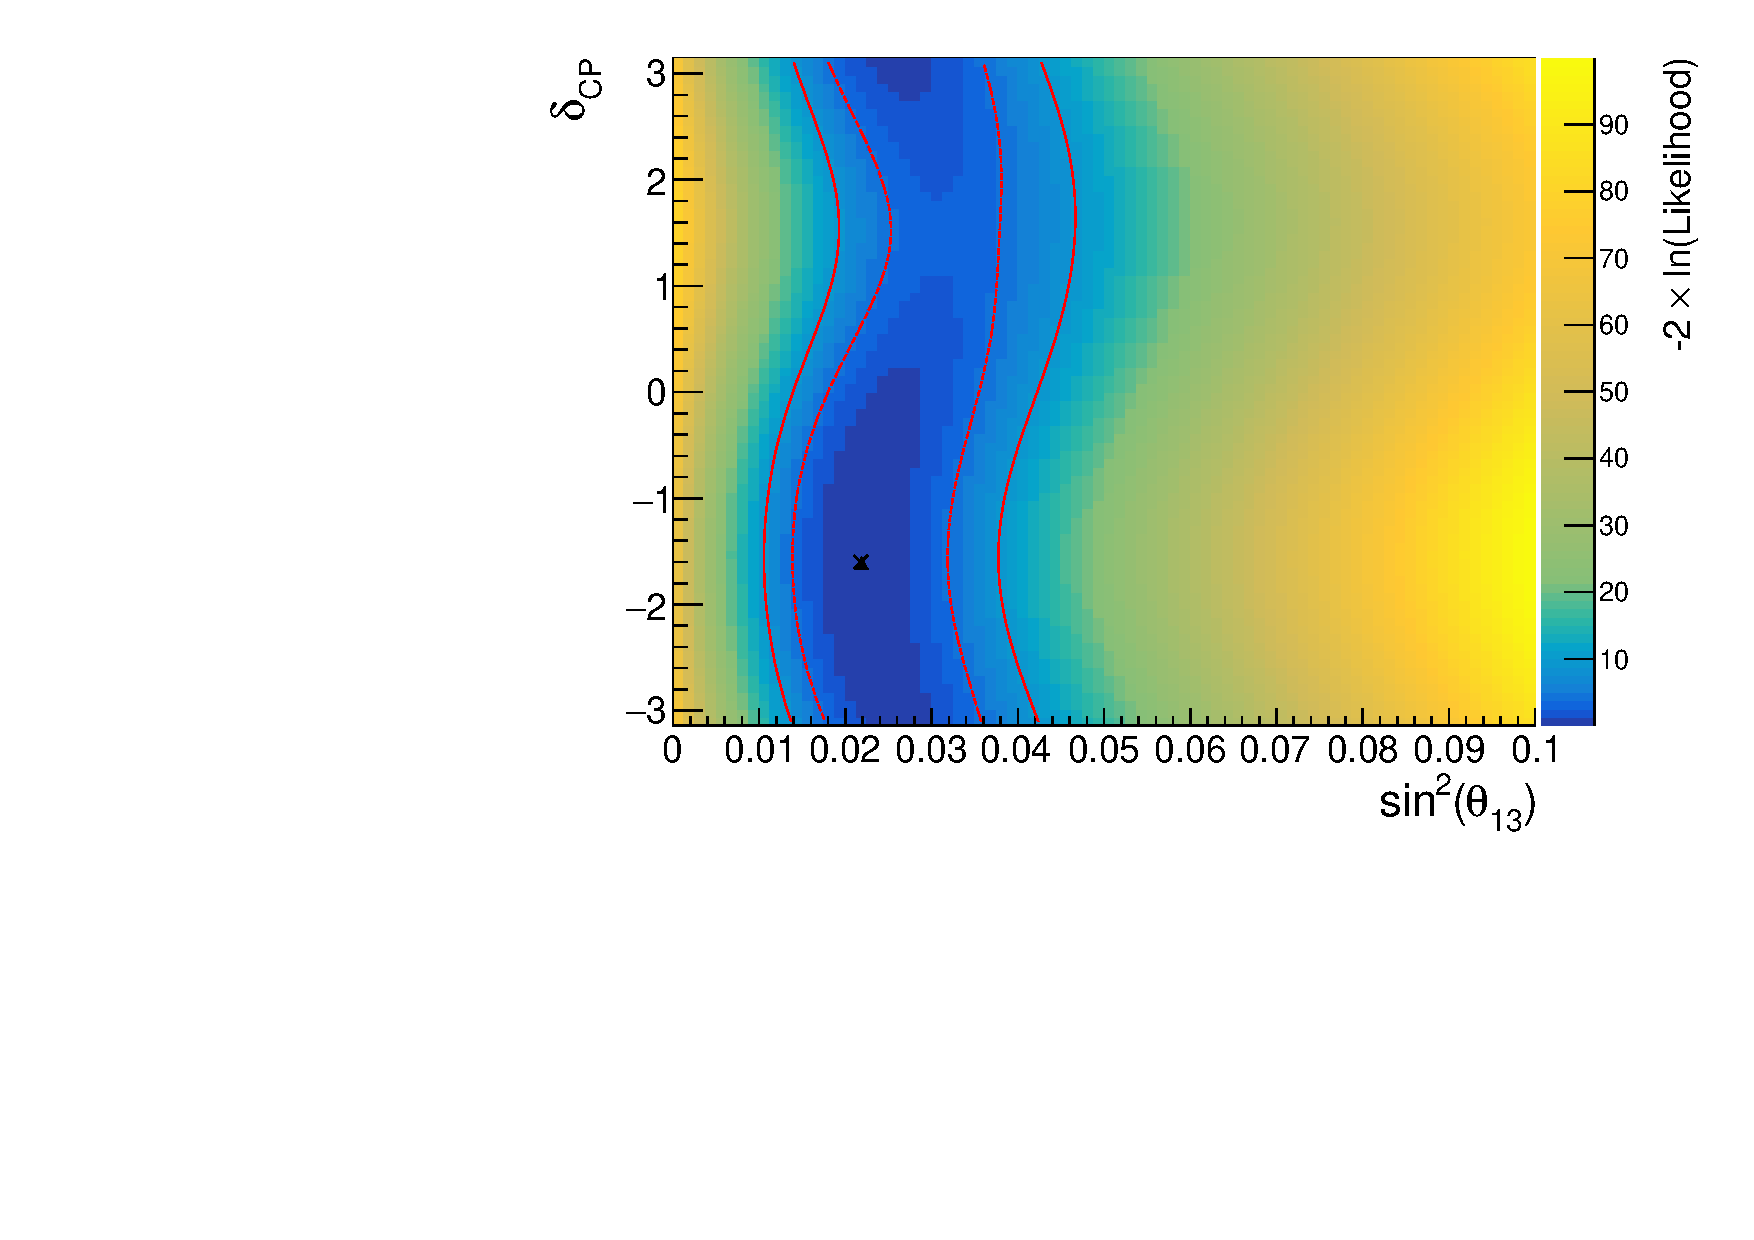
\includegraphics[width=\textwidth, trim={0mm 0mm 0mm 0mm}, clip,page=1]{Figures/OA/AppearanceScans.pdf}
  \end{subfigure}%
  \begin{subfigure}[t]{0.5\textwidth}
    \subcaption{Atmospheric Samples}
    \includegraphics[width=\textwidth, trim={0mm 0mm 0mm 0mm}, clip,page=2]{Figures/OA/AppearanceScans.pdf}
  \end{subfigure}
  \begin{subfigure}[t]{1.0\textwidth}
    \subcaption{All Samples}
    \includegraphics[width=\textwidth, trim={0mm 0mm 0mm 0mm}, clip,page=3]{Figures/OA/AppearanceScans.pdf}
  \end{subfigure}
  \caption{Two-dimensional log-likelihood scan of the appearance (\quickmath{\sin^{2}(\theta_{13})}\text{\textendash}\quickmath{\delta_{CP}}) parameters showing the response of the beam samples (top left), atmospheric samples (top right) and the summed response (bottom). The Asimov A oscillation parameters, defined in \autoref{tab:Theory_ParameterSets}, are known to be the true point (Black Cross). The position of the smallest log-likelihood is highlighted with the triangle. Prior uncertainty terms of the oscillation parameters are neglected. The two(three) sigma contour levels are illustrated with the dashed(solid) red line.}
  \label{fig:OscillationAnalysis_2DLLHOscScans_App}
\end{figure}

\begin{figure}[h]
  \begin{subfigure}[t]{0.5\textwidth}
    \subcaption{Beam Samples}
    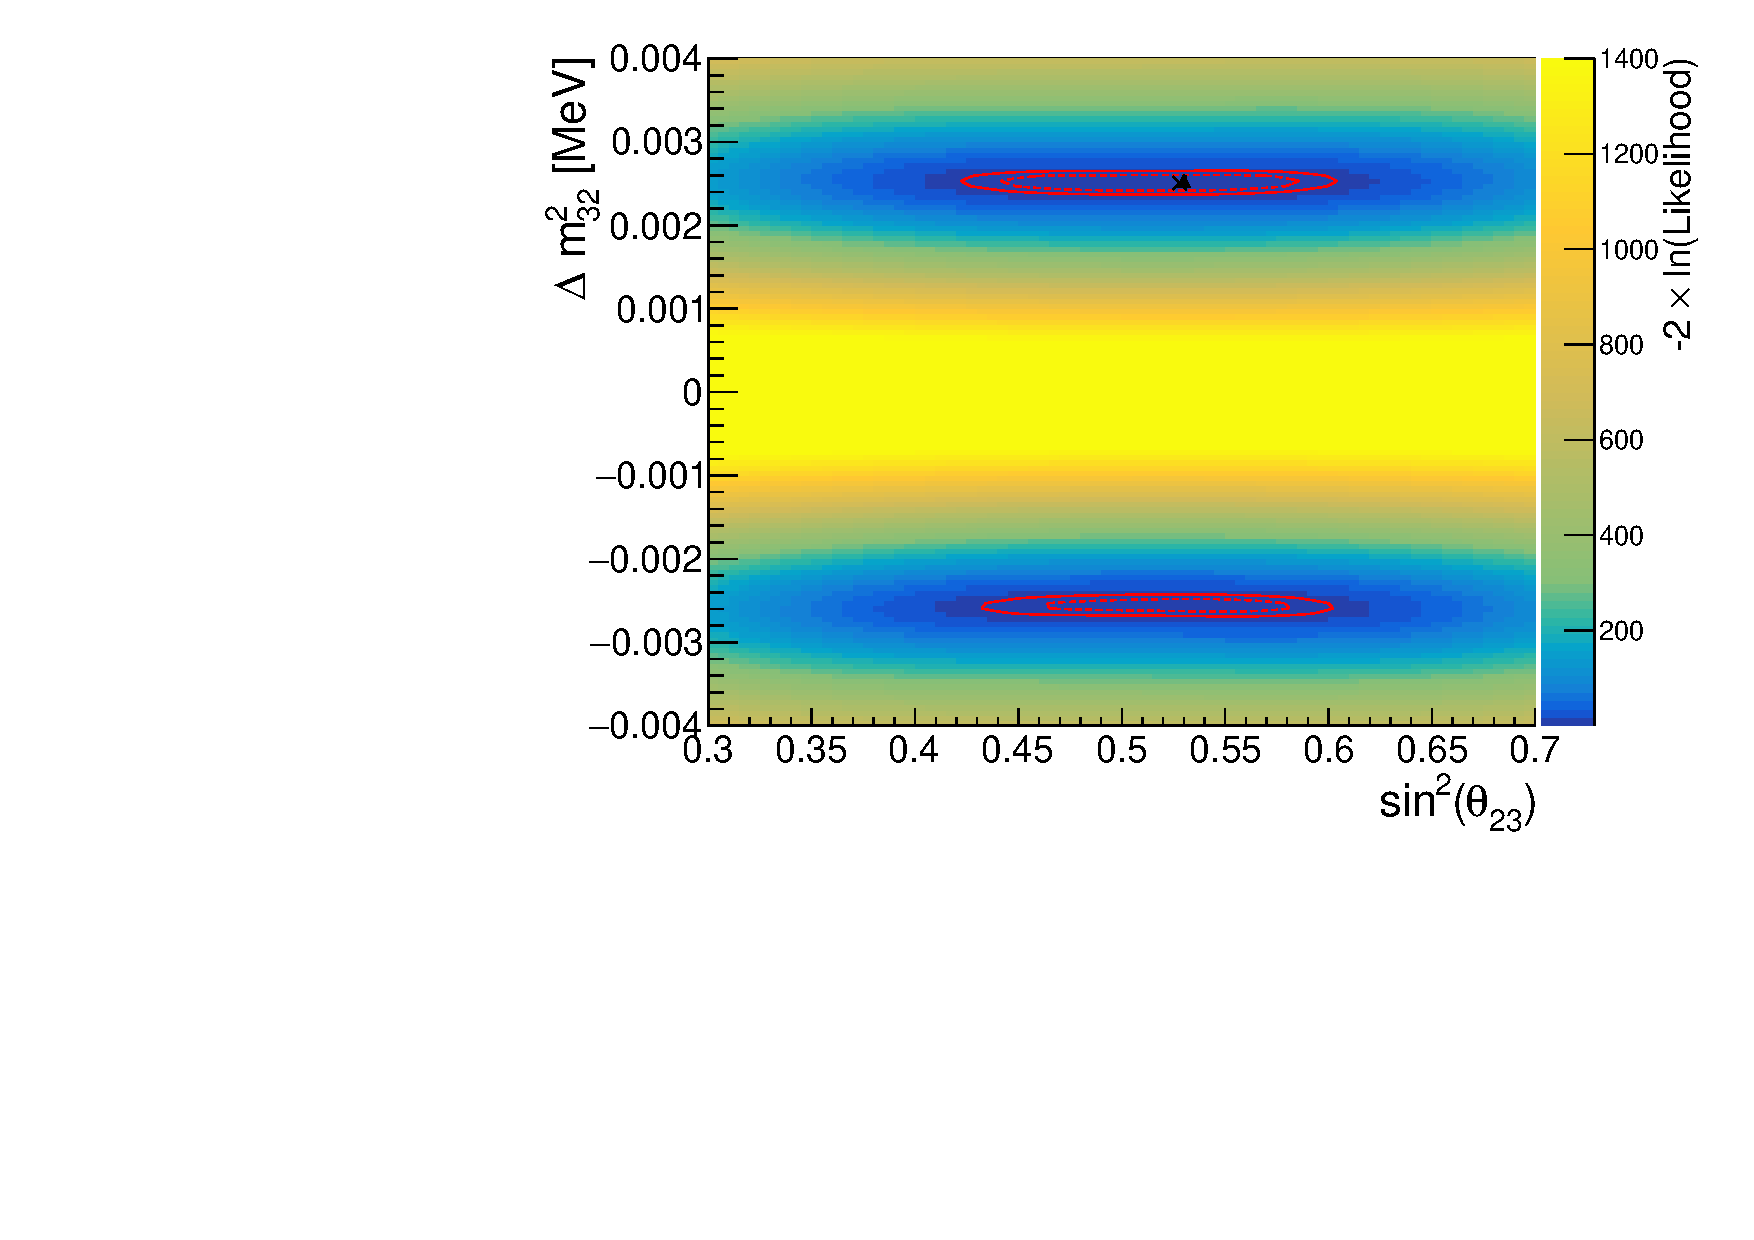
\includegraphics[width=\textwidth, trim={0mm 0mm 0mm 0mm}, clip,page=1]{Figures/OA/DisappearanceScans.pdf}
  \end{subfigure}%
  \begin{subfigure}[t]{0.5\textwidth}
    \subcaption{Atmospheric Samples}
    \includegraphics[width=\textwidth, trim={0mm 0mm 0mm 0mm}, clip,page=2]{Figures/OA/DisappearanceScans.pdf}
  \end{subfigure}
  \begin{subfigure}[t]{1.0\textwidth}
    \subcaption{All Samples}
    \includegraphics[width=\textwidth, trim={0mm 0mm 0mm 0mm}, clip,page=3]{Figures/OA/DisappearanceScans.pdf}
  \end{subfigure}
  \caption{Two-dimensional log-likelihood scan of the disappearance (\quickmath{\sin^{2}(\theta_{23})}\text{\textendash}\quickmath{\Delta m^{2}_{32}}) parameters showing the response of the beam samples (top left), atmospheric samples (top right) and the summed response (bottom). The Asimov A oscillation parameters, defined in \autoref{tab:Theory_ParameterSets}, are known to be the true point (Black Cross). The position of the smallest log-likelihood is highlighted with the triangle. Prior uncertainty terms of the oscillation parameters are neglected. The two(three) sigma contour levels are illustrated with the dashed(solid) red line.}
  \label{fig:OscillationAnalysis_2DLLHOscScans_Dis}
\end{figure}

\clearpage

The likelihood scans illustrated thus far only consider the sensitivity of this analysis for a fixed set of true oscillation parameters, namely Asimov A defined in \autoref{tab:Theory_ParameterSets}. Whilst computationally infeasible to run many fits at different parameter sets, it is possible to calculate the likelihood response to different Asimov data sets. \autoref{fig:OscillationAnalysis_AsimovEval_DCP} and \autoref{fig:OscillationAnalysis_AsimovEval_TH23} illustrate how the sensitivity changes for differing true values of \quickmath{\delta_{CP}} and \quickmath{\sin^{2}(\theta_{23})}, respectively. For both of these plots, the other oscillation parameters are fixed at their Asimov A values. Consequently, the caveat of fixed systematic parameters and correlations between other oscillation parameters being neglected still applies.

To explain how these plots are made, consider \autoref{fig:OscillationAnalysis_AsimovEval_DCP}. This plot is built by considering multiple one-dimensional log-likelihood scans, each creating an Asimov data set with the value of \quickmath{\delta_{CP}} taken from the x-axis. The likelihood to this particular Asimov data set is calculated after reweighting the Monte Carlo prediction to each value of \quickmath{\delta_{CP}} on the y-axis.

\autoref{fig:OscillationAnalysis_AsimovEval_DCP} illustrates the sensitivity to \quickmath{\delta_{CP}}. To interpret this plot, larger contours result in more parameter space being excluded from the \quickmath{1\sigma} region. The \quickmath{1\sigma} intervals contain regions where the beam and atmospheric samples have discontinuous contours. For example, for the x-axis value of \quickmath{\delta_{CP} = 0}, the beam samples sensitivity would include two discontinuous regions excluded from the \quickmath{1\sigma} interval: \quickmath{\delta_{CP} \sim 0} and \quickmath{\delta_{CP} \sim \pi}. This behaviour is also seen in atmospheric samples response but at a value of \quickmath{\delta_{CP} \sim -1}. This difference allows the joint fit to have increased sensitivity to these regions. Consequently, the difference between the beam-only and joint beam-atmospheric fit should be studied using multiple Asimov data sets.

Despite the increased sensitivity at \quickmath{1\sigma}, the \quickmath{2\sigma} intervals from the joint fit are more similar to the two independent sensitivities and the off-diagonal degeneracies mostly remain. This indicates that the joint fit has the strength to aid parameter determination but can not entirely break the degeneracies in \quickmath{\delta_{CP}} at higher confidence levels. 

\autoref{fig:OscillationAnalysis_AsimovEval_TH23} illustrates a similar analysis as above, although the value of \quickmath{\sin^{2}(\theta_{23})} is varied and \quickmath{\delta_{CP}} is fixed to the Asimov A parameter value. Due to the beam parameters and baseline being tuned to specifically target this oscillation parameter, the average sensitivity of the beam samples is stronger than the atmospheric samples. However, the degeneracy around maximal mixing (\quickmath{\sin^{2}(\theta_{23}) = 0.5}) is significantly more peaked in the beam samples compared to the atmospheric samples. This means that a value of \quickmath{\sin^{2}(\theta_{23}) \sim 0.56} would be contained within the \quickmath{1\sigma} confidence interval for a true value of \quickmath{\sin^{2}(\theta_{23}) \sim 0.46} if using the beam-only analysis, whereas it would be excluded in the joint analysis.

This behaviour is strengthened when considering the \quickmath{2\sigma} intervals, to the point where two distinct discontinuous regions of the \quickmath{2\sigma} intervals exist around the Asimov point \quickmath{\sin^{2}(\theta_{23}) \sim 0.41, 0.6}. Given the caveat of only considering likelihood scans, the joint analysis would mostly eliminate the discontinuous intervals in these regions. This means that the joint fit could feasibly have an increased preference for the correct octant hypothesis.

\begin{figure}[h]
  \begin{subfigure}[t]{1.0\textwidth}
    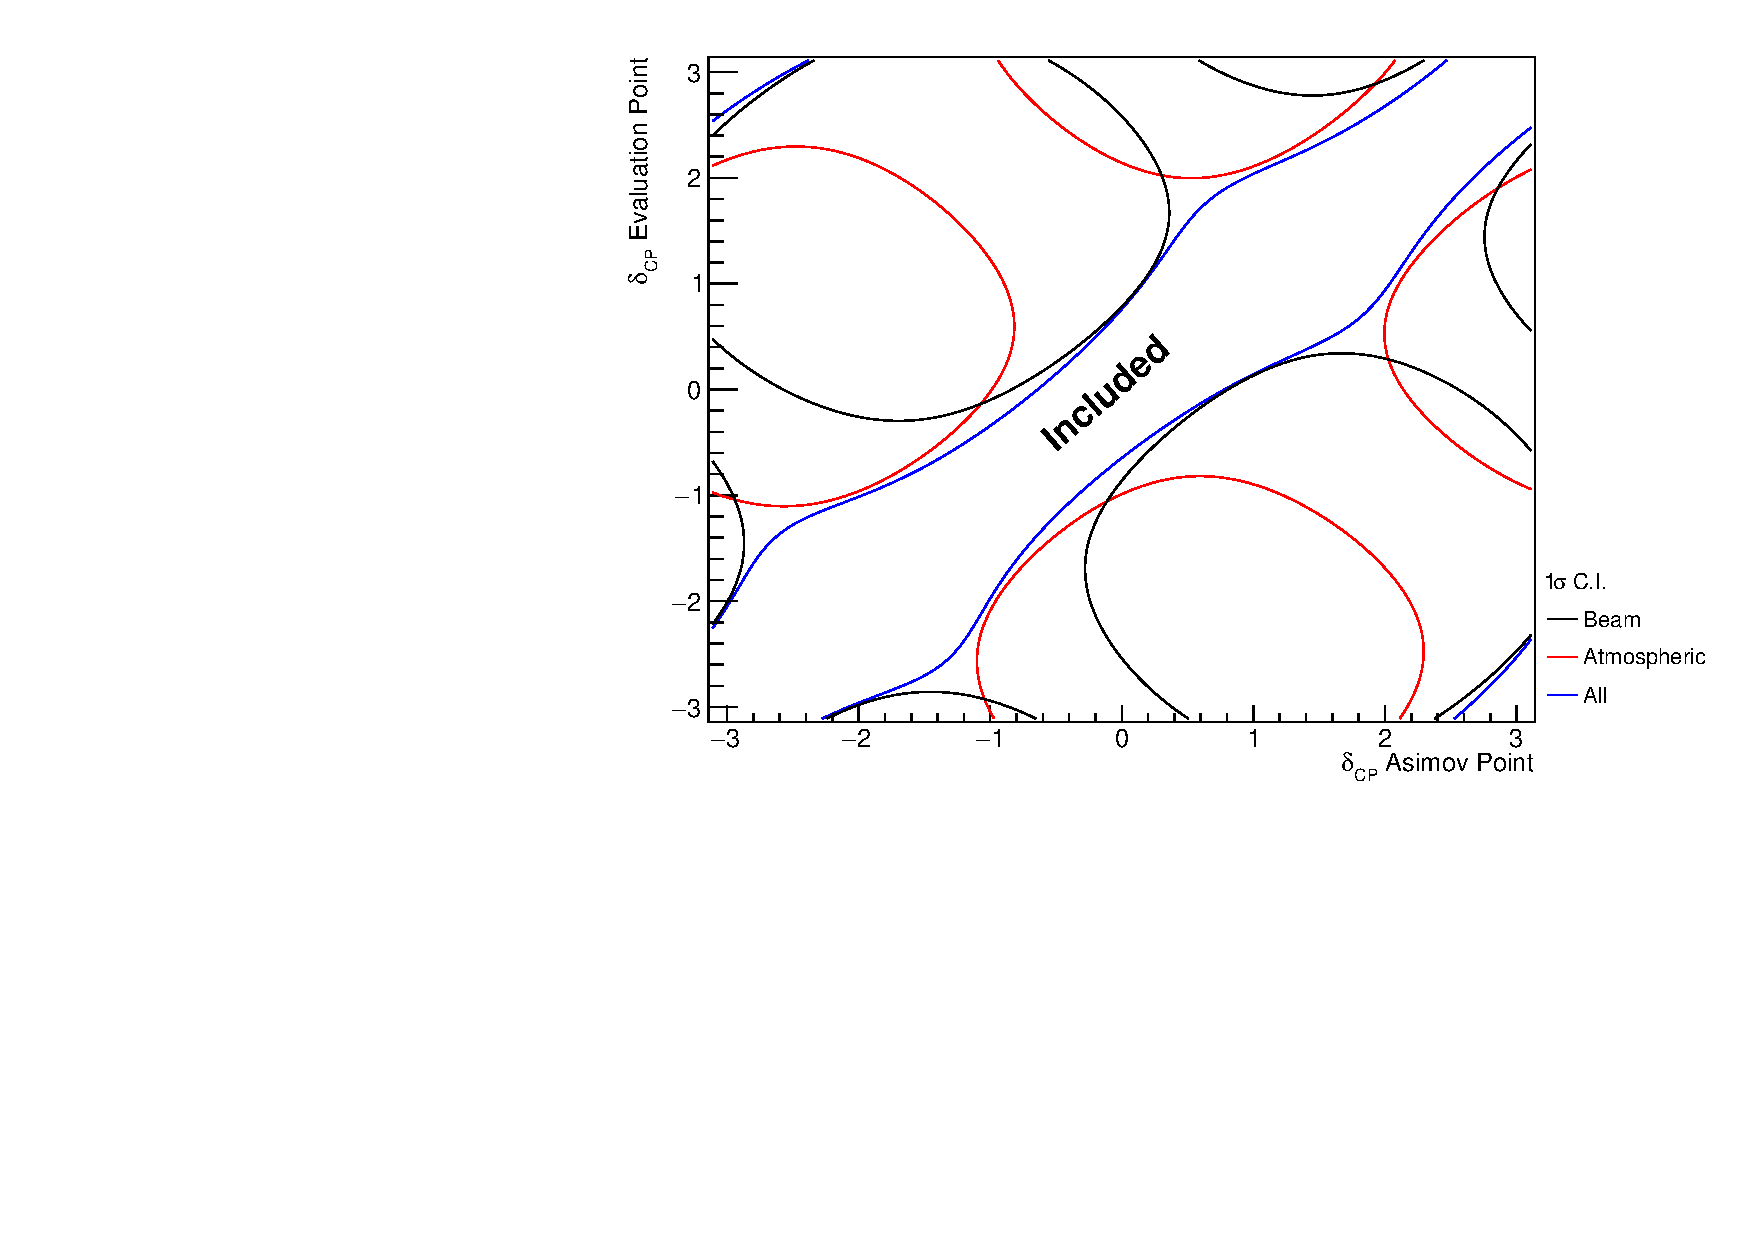
\includegraphics[width=\textwidth, trim={0mm 0mm 0mm 0mm}, clip,page=1]{Figures/OA/DCP_Scans_1Sig.pdf}
  \end{subfigure}
  \begin{subfigure}[t]{1.0\textwidth}
    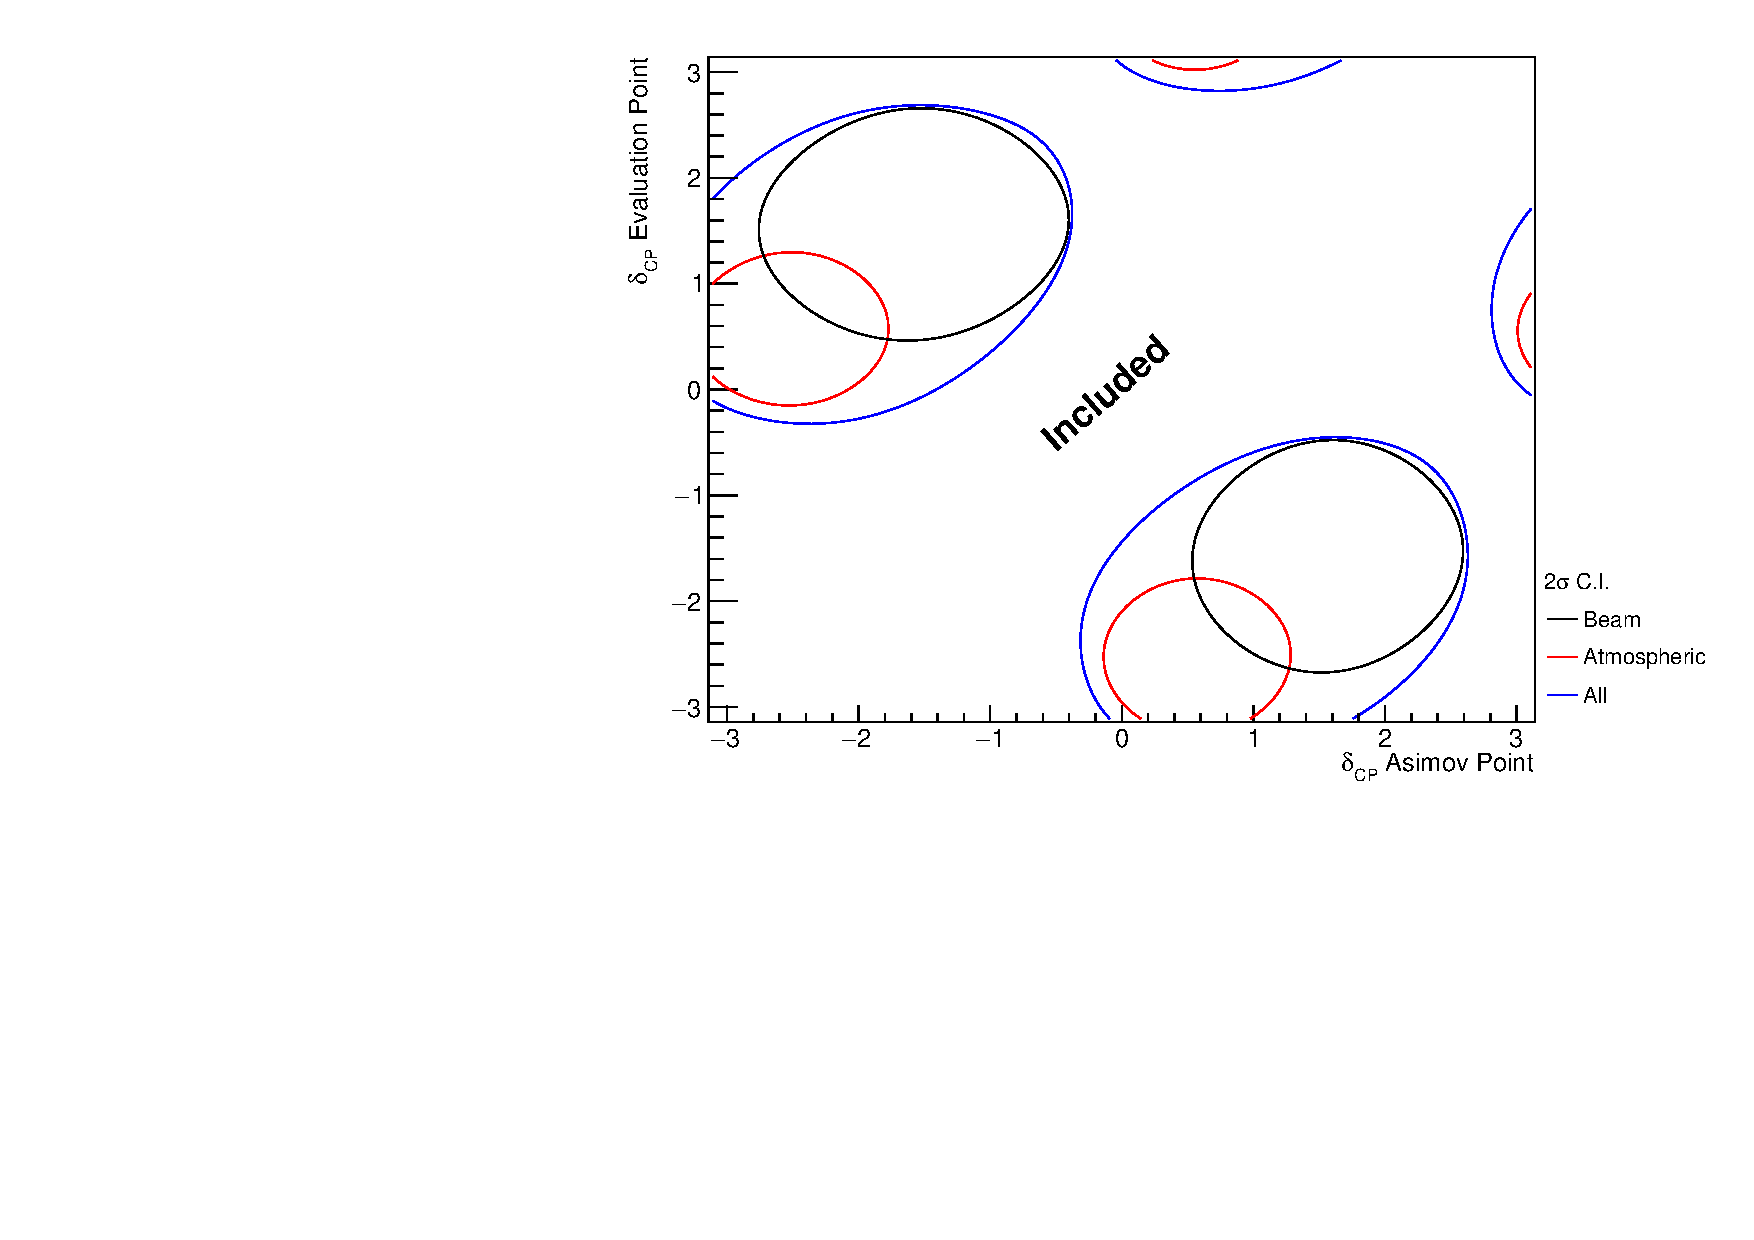
\includegraphics[width=\textwidth, trim={0mm 0mm 0mm 0mm}, clip,page=1]{Figures/OA/DCP_Scans_2Sig.pdf}
  \end{subfigure}
  \caption{A series of one-dimensional likelihood scans over \quickmath{\delta_{CP}}, where an Asimov data set is built for each value of \quickmath{\delta_{CP}} on the x-axis and the likelihood is evaluated for each value of \quickmath{\delta_{CP}} on the y-axis. The diagonal represents the minimum log-likelihood and defines the region included within the \quickmath{1\sigma} (Top) and \quickmath{2\sigma} (Bottom) confidence intervals. The beam (black) and atmospheric (red) samples are individually plotted and the joint fit (blue) is the sum of the two.}
  \label{fig:OscillationAnalysis_AsimovEval_DCP}
\end{figure}

\begin{figure}[h]
  \begin{subfigure}[t]{1.0\textwidth}
    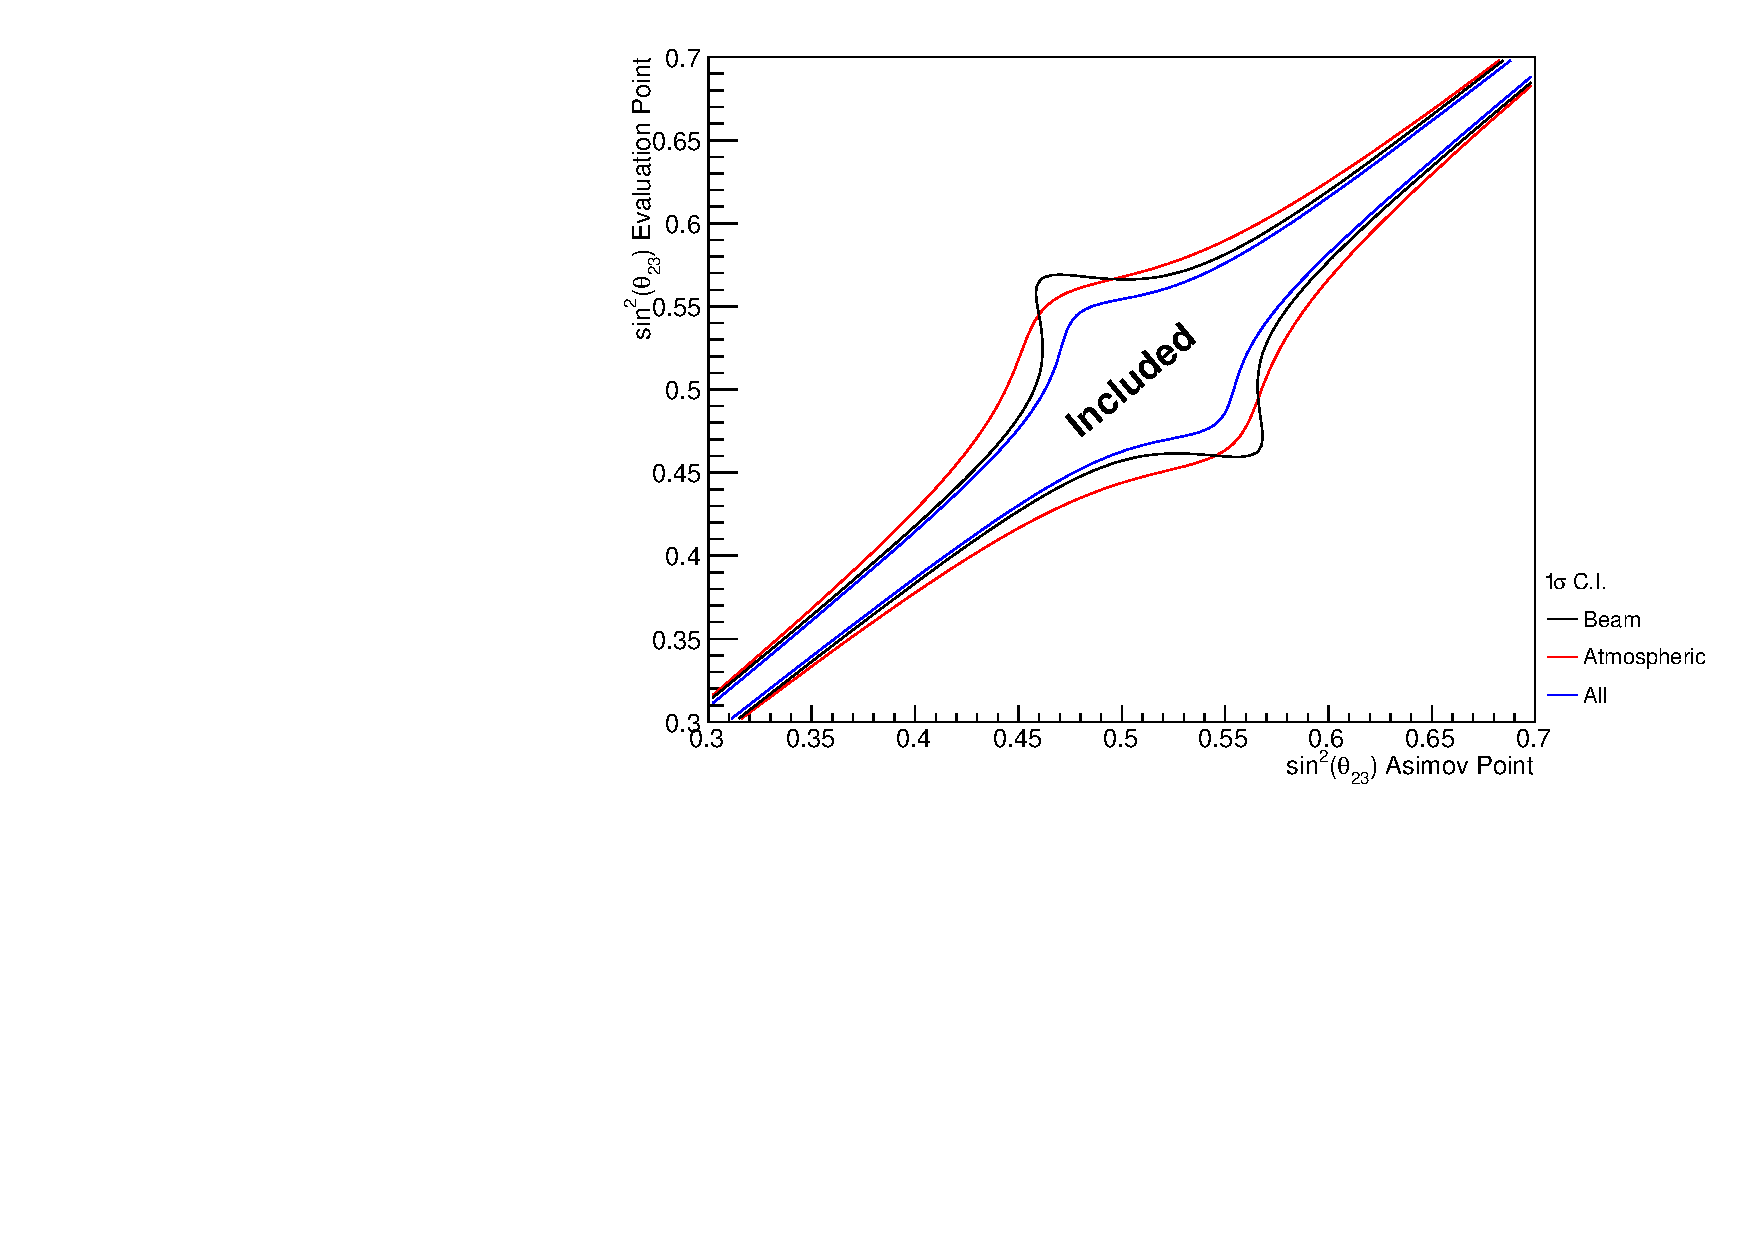
\includegraphics[width=\textwidth, trim={0mm 0mm 0mm 0mm}, clip,page=1]{Figures/OA/TH23_Scans_1Sig.pdf}
  \end{subfigure}                                                                                                                                                                                          
  \begin{subfigure}[t]{1.0\textwidth}
    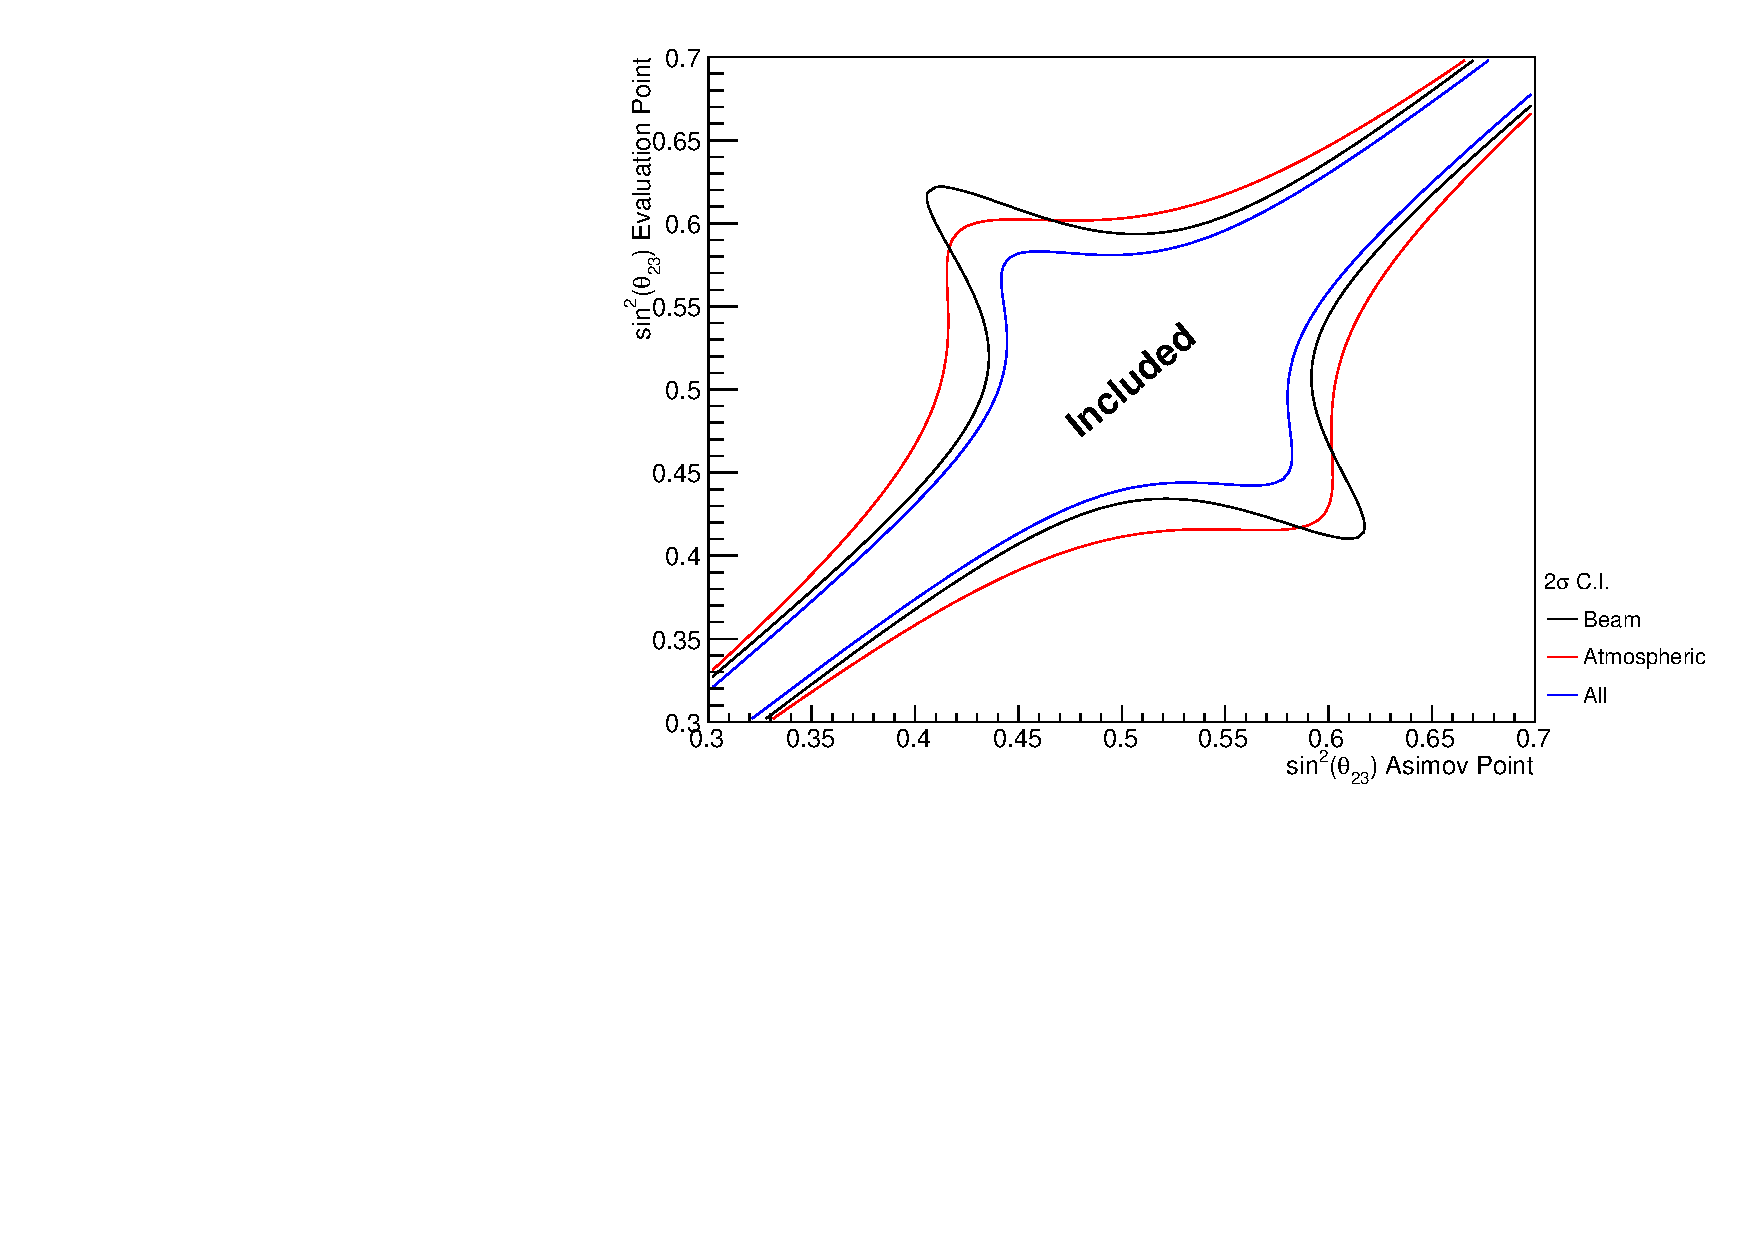
\includegraphics[width=\textwidth, trim={0mm 0mm 0mm 0mm}, clip,page=1]{Figures/OA/TH23_Scans_2Sig.pdf}
  \end{subfigure}
  \caption{A series of one-dimensional likelihood scans over \quickmath{\sin^{2}(\theta_{23})}, where an Asimov data set is built for each value of \quickmath{\sin^{2}(\theta_{23})} on the x-axis and the likelihood is evaluated for each value of \quickmath{\sin^{2}(\theta_{23})} on the y-axis. The diagonal represents the minimum log-likelihood and defines the region included within the \quickmath{1\sigma} (Top) and \quickmath{2\sigma} (Bottom) confidence intervals. The beam (black) and atmospheric (red) samples are individually plotted and the joint fit (blue) is the sum of the two.}
  \label{fig:OscillationAnalysis_AsimovEval_TH23}
\end{figure}

\clearpage

Alongside oscillation parameters (\autoref{fig:OscillationAnalysis_LLHScanOscPars}), the sensitivity to systematic parameters can also be studied for the joint fit. As some of these parameters are correlated between the beam and atmospheric events, the response of the atmospheric samples can modify the constraint. This means the systematics can have additional constraints than they would from a beam-only analysis. Therefore, the response from the beam and the atmospheric samples to various systematic parameters has been compared in \autoref{fig:OscillationAnalysis_LLHScanSystPars}. The Asimov data set has been created using the AsimovA oscillation parameter and the pre-fit systematic tune. For example, the systematic parameter controlling the effective axial mass coupling in CCQE interactions, \quickmath{M_{A}^{QE}}, is clearly dominated by the ND constraint. An example where the response of the atmospheric sample is approximately similar to the near detector constraint is the \text{2p2h CtoO} normalisation systematic. This systematic models the scaling of the 2p2h interaction cross-section on a carbon target to an oxygen target. There are also systematics that have no near detector constraint. For example, the systematic parameters which describe the normalisation of the NC1Gamma and NCOther interaction modes. The atmospheric and beam samples can have similar sensitivity to these systematics due to their similar composition in energy and interaction mode. As an example of how the atmospheric samples can help constrain systematic parameters used within the T2K-only analysis, these NC background events in beam electron-like samples will be more constrained with the additional sensitivity of atmospheric samples. This would be expected to reduce the overall uncertainty of the beam electron-like event rates in the joint analysis compared to the beam-only studies. This could modify the sensitivity of the beam samples due to the more constrained background events.

\begin{figure}[h]
  \begin{subfigure}[t]{0.5\textwidth}
    \includegraphics[width=\textwidth, trim={0mm 0mm 0mm 0mm}, clip,page=2]{Figures/OA/LLHScans_Systs.pdf}
    \subcaption{\quickmath{M_{A}^{QE}}}
  \end{subfigure}%
  \begin{subfigure}[t]{0.5\textwidth}
    \includegraphics[width=\textwidth, trim={0mm 0mm 0mm 0mm}, clip,page=5]{Figures/OA/LLHScans_Systs.pdf}
    \subcaption{\text{2p2h CtoO} Norm.}
  \end{subfigure}
  \begin{subfigure}[t]{0.5\textwidth}
    \includegraphics[width=\textwidth, trim={0mm 0mm 0mm 0mm}, clip,page=41]{Figures/OA/LLHScans_Systs.pdf}
    \subcaption{NC1Gamma Norm.}
  \end{subfigure}%
  \begin{subfigure}[t]{0.5\textwidth}
    \includegraphics[width=\textwidth, trim={0mm 0mm 0mm 0mm}, clip,page=43]{Figures/OA/LLHScans_Systs.pdf}
    \subcaption{NC Other SK Norm.}
  \end{subfigure}
  \begin{subfigure}[t]{0.5\textwidth}
    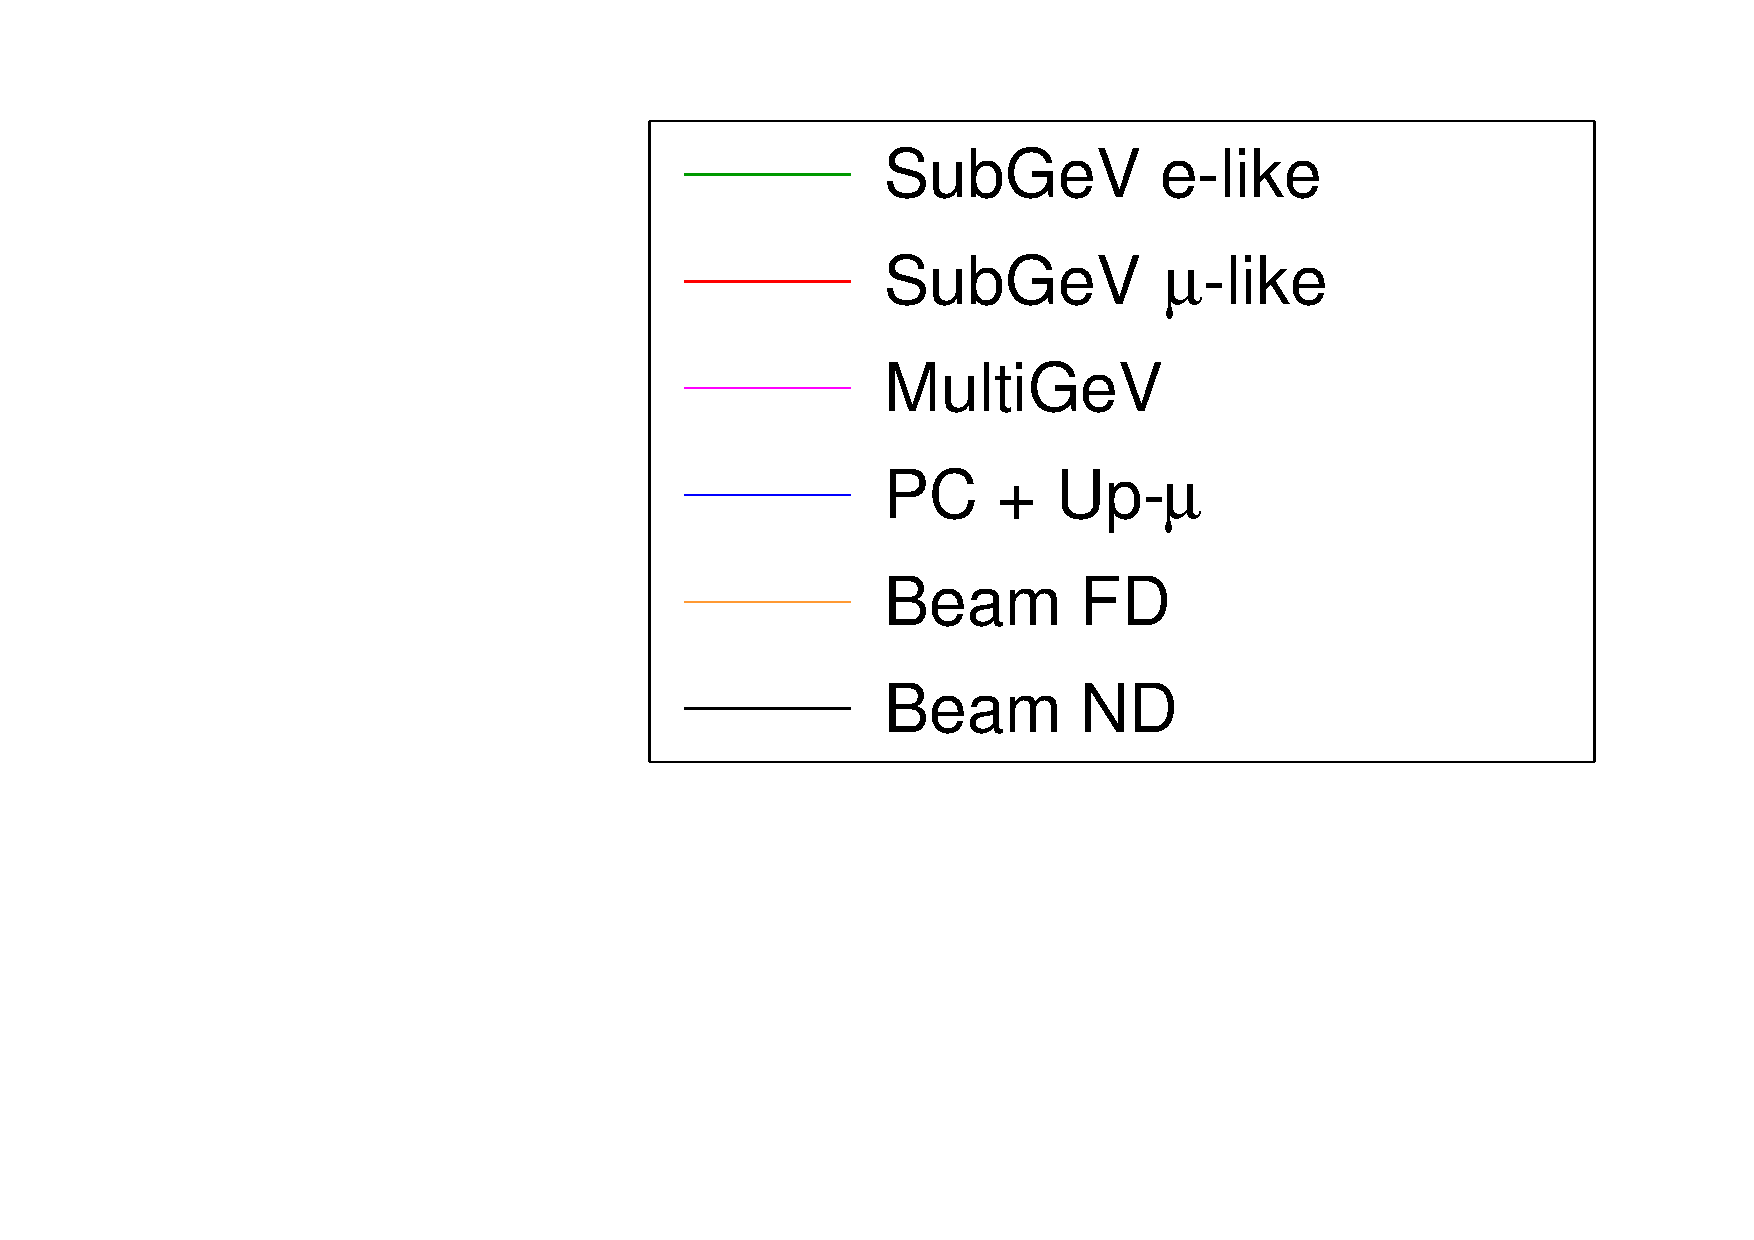
\includegraphics[width=\textwidth, trim={0mm 0mm 0mm 0mm}, clip,page=1]{Figures/OA/LLHScans_Systs.pdf}
  \end{subfigure}
  \caption{The response of the likelihood, as defined in section 8.2, illustrating the response of the samples to the various cross-section systematic parameters.}
  \label{fig:OscillationAnalysis_LLHScanSystPars}
\end{figure}

\clearpage
\section{Sensitivity Studies}
\label{sec:OscillationAnalysis_Sensitivities}

The sensitivities of the joint T2K and SK oscillation analysis are presented in the form of Asimov fits. These fits consider beam samples from the near and far detector alongside atmospheric samples at SK. This technique builds an Asimov data set (following \autoref{sec:OscillationAnalysis_LLHCalc}) using the AsimovA oscillation parameters and post-BANFF systematic tune, which is then fit. This technique eliminates statistical fluctuations from the data, therefore, providing the maximum sensitivity of the analysis.

In practice, the Asimov fits presented within this analysis are modified from the above definition. An Asimov prediction of both beam and atmospheric far detector samples is fit whilst the true data is used for near detector samples. The Asimov predictions at the far detector are built using the post-BANFF tune (as discussed in \autoref{sec:T2KSKExp_T2K}). These modifications mean that the results are equivalent to performing a far detector Asimov fit using inputs from the BANFF data fit. Consequently, this allows the results to be cross-checked with the results from the P-Theta analysis. The comparison has been performed and is documented in \cite{barrow_M3_PT_Comp}. No significant discrepancies were found between the fitters.

This section proceeds with the following studies. Firstly, the sensitivity of the atmospheric samples using the correlated detector model is detailed in \autoref{sec:OscillationAnalysis_SKOnly}. This includes studying the choice of applying the 2020 PDG reactor constraint \cite{Particle_Data_Group2020-ms} to the atmospheric samples, which is documented in \autoref{sec:OscillationAnalysis_SKOnly_wRC}. Additionally, the effect of applying the near-detector constraints onto the atmospheric samples is discussed in \autoref{sec:OscillationAnalysis_SKOnly_NoND}. The main result is the sensitivity of the simultaneous beam and atmospheric fit. The sensitivities, both with and without the application of the reactor constraint, are presented in \autoref{sec:OscillationAnalysis_JointFit} and \autoref{sec:OscillationAnalysis_JointFit_wRC}, respectively. To indicate the benefit of the joint analysis, the sensitivities are compared to the 2020 T2K beam-only sensitivities \cite{Dunne2020-uf, t2k_tn_393} in \autoref{sec:OscillationAnalysis_JointFit_OA2020} and \autoref{sec:OscillationAnalysis_JointFit_OA2020_wRC}. The T2K analysis is used as a reference as it uses the same samples and a similar systematic model. As shown in \autoref{sec:OscillationAnalysis_LLHScans}, the response of the beam and atmospheric samples change depending upon the true set of oscillation parameters assumed. Therefore, \autoref{sec:OscillationAnalysis_AsimovB} documents the sensitivities at an alternative oscillation parameter set. These results have been presented at the Neutrino 2022 conference on behalf of the T2K and SK collaborations \cite{Bronner2022-wd}.

\subsection{Atmospheric-Only Sensitivity Without Reactor Constraint}
\label{sec:OscillationAnalysis_SKOnly}

This section presents the results of an Asimov fit using samples from the near detector and only atmospheric samples from the far detector. The results are presented as one-dimensional or two-dimensional histograms which have been marginalised over all other parameters using the technique outlined in \autoref{sec:MarkovChainMonteCarlo_Marginalisation}. Each histogram displays the posterior probability density and illustrates the credible intervals, calculated using the technique in \autoref{sec:MarkovChainMonteCarlo_ParameterEstimation}. For this fit, a flat prior is used for \quickmath{\sin^{2}(\theta_{13})} meaning that the reactor constraint is not applied. The Asimov data is generated assuming the AsimovA oscillation parameter set defined in \autoref{tab:Theory_ParameterSets} and the post-BANFF systematic parameter tune.

\begin{figure}[h]
  \begin{subfigure}[t]{0.98\textwidth}
    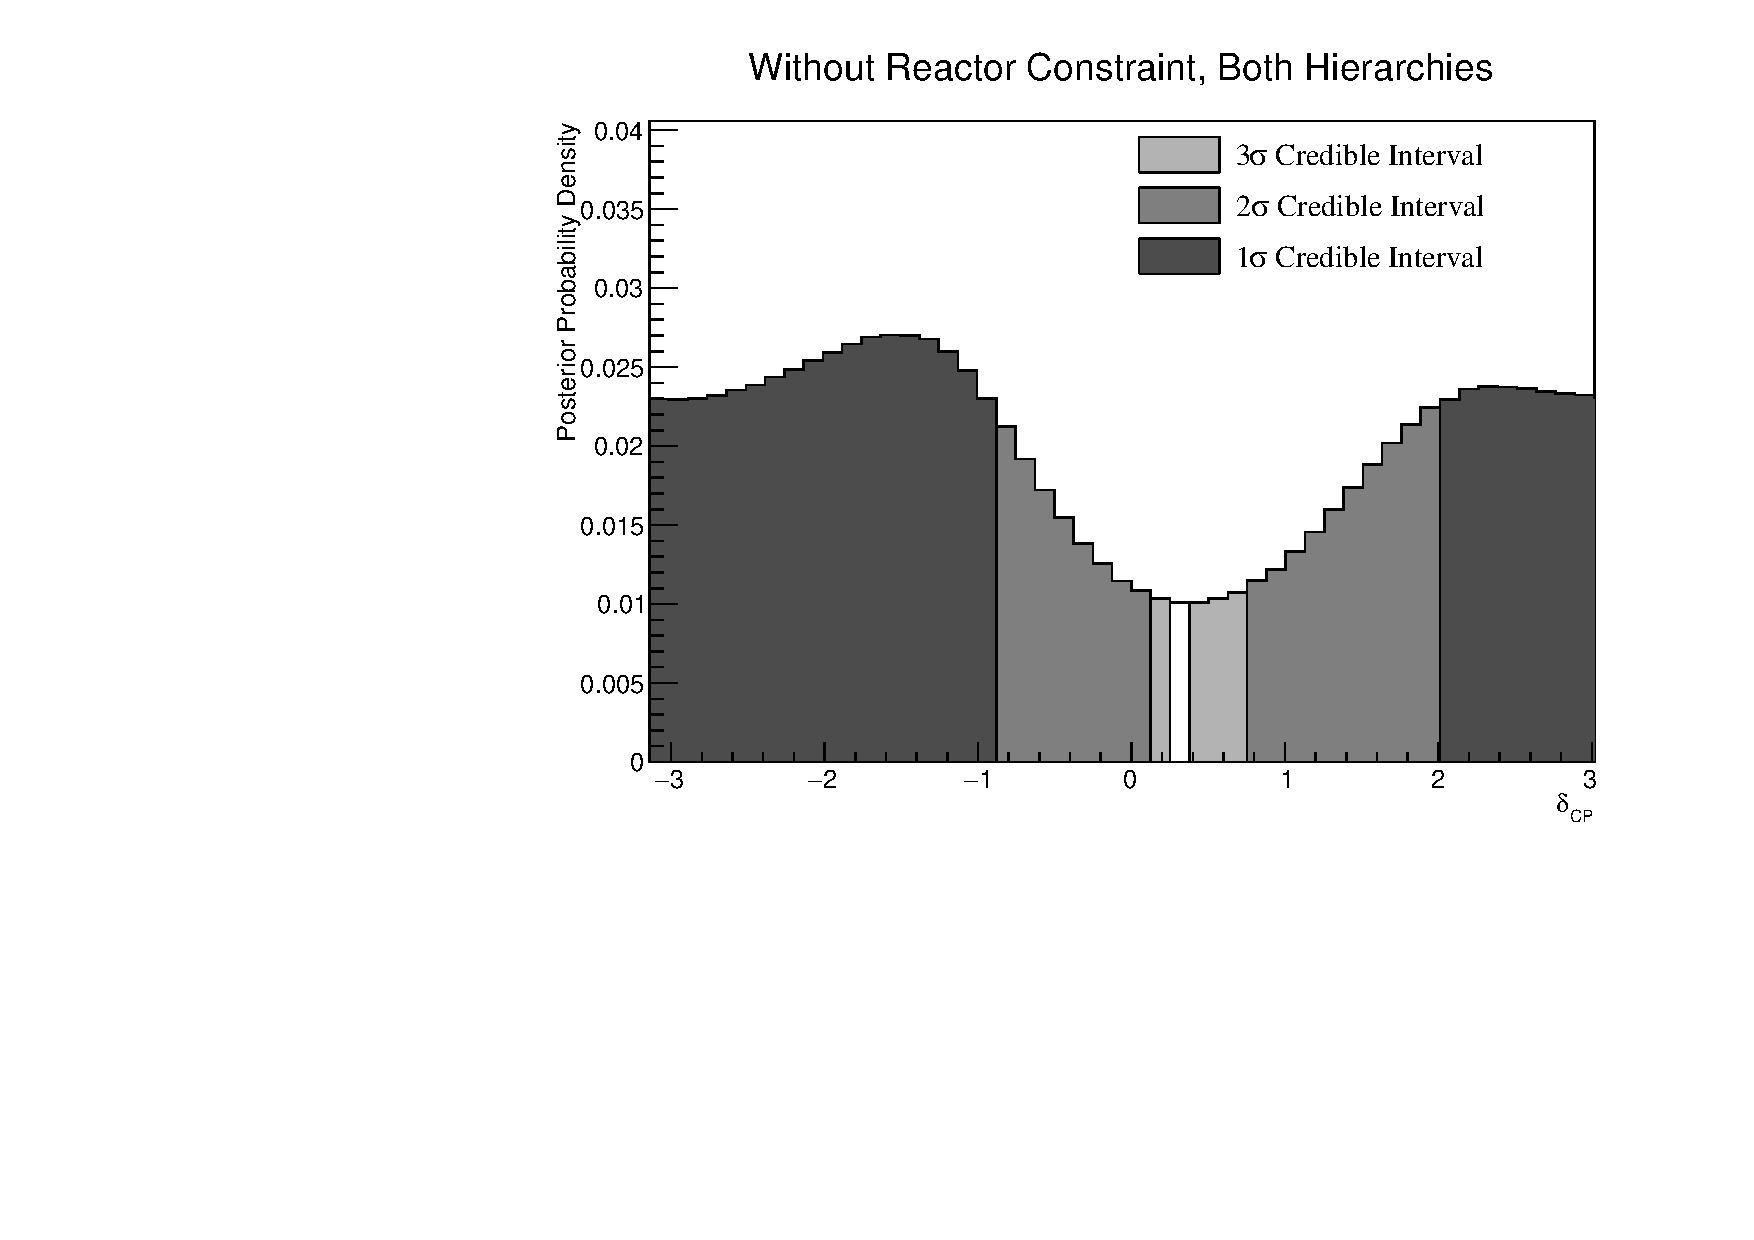
\includegraphics[width=\textwidth, trim={0mm 0mm 0mm 0mm}, clip,page=1]{Figures/OA/SKOnlyFit/Contours_1D_dcp_BH_1_woRC_UnSmeared_CredibleInterval.pdf}
  \end{subfigure}
  \caption{The one-dimensional posterior probability density distribution in \quickmath{\delta_{CP}}, marginalised over both hierarchies, from the SK atmospheric-only fit. The reactor constraint is not applied. The vertical dashed line represents the known value of \quickmath{\delta_{CP}}.}
  \label{fig:OscillationAnalysis_SKOnly_DCP}
\end{figure}

\autoref{fig:OscillationAnalysis_SKOnly_DCP} illustrates the posterior probability density for \quickmath{\delta_{CP}}, marginalised over both hierarchies.
%If instead, only steps in the normal hierarchy were considered, the shape of the contours would change.
The fit favours the known oscillation parameter (\quickmath{\delta_{CP} = -1.601}) although the posterior probability is very flat through the range of \quickmath{-\pi < \delta_{CP} < -1} and \quickmath{2 < \delta_{CP} < \pi}. There is also a region around \quickmath{\delta_{CP} \sim 0.4} which is disfavoured at \quickmath{2\sigma}. This indicates that the SK samples can rule out some parts of the CP conserving parameter space reasonably well, near \quickmath{\delta_{CP} \sim 0.4}, when the true value of \quickmath{\delta_{CP} \sim -\pi/2}.

\begin{figure}[h]
  \begin{subfigure}[t]{0.98\textwidth}
    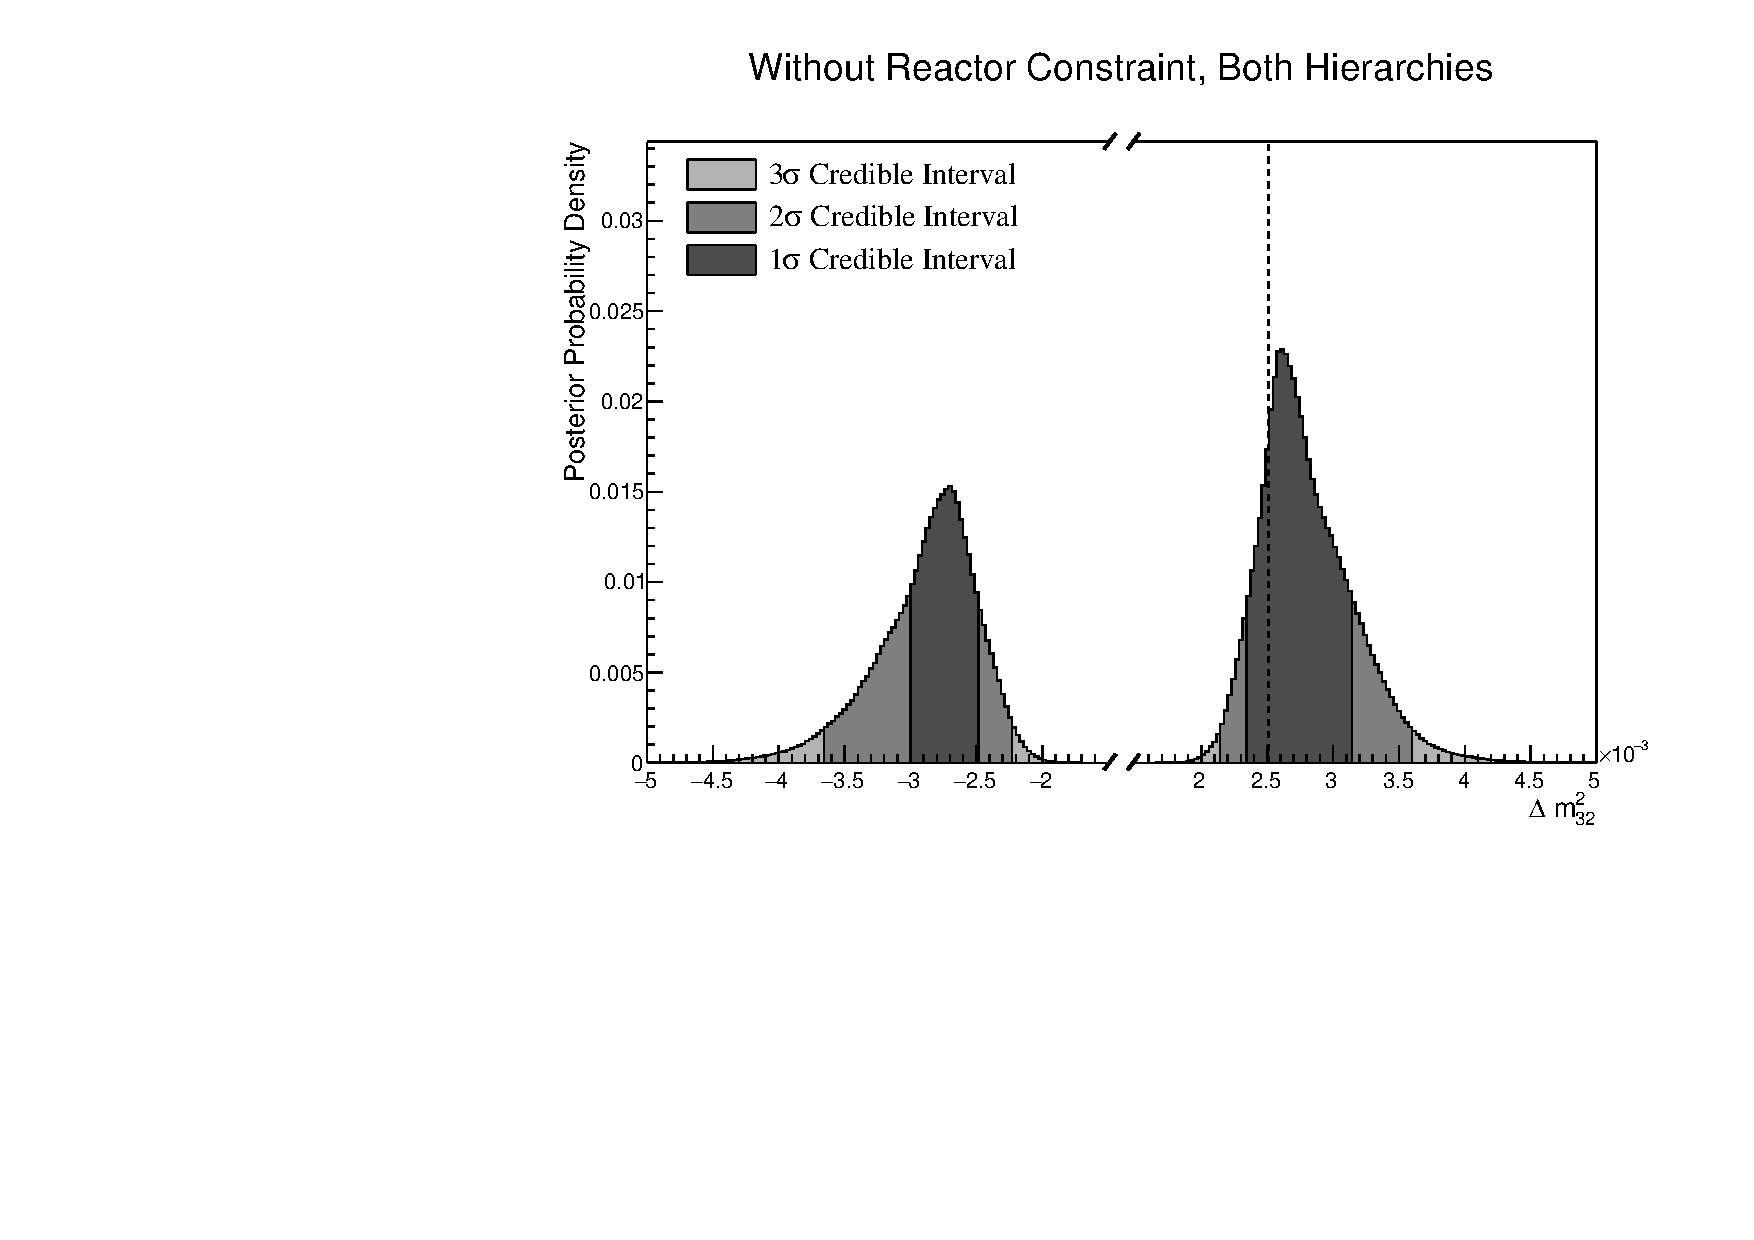
\includegraphics[width=\textwidth, trim={0mm 0mm 0mm 0mm}, clip,page=1]{Figures/OA/SKOnlyFit/Contours_1D_dm32_BH_1_woRC_UnSmeared_CredibleInterval.pdf}
  \end{subfigure}
  \caption{The one-dimensional posterior probability density distribution in \quickmath{\Delta m^{2}_{32}}, marginalised over both hierarchies, from the SK atmospheric-only fit. The reactor constraint is not applied. The vertical dashed line represents the known value of \quickmath{\Delta m^{2}_{32}}.}
  \label{fig:OscillationAnalysis_SKOnly_DM32}
\end{figure}

The posterior probability density in \quickmath{\Delta m^{2}_{32}} is given in \autoref{fig:OscillationAnalysis_SKOnly_DM32}. This distribution includes steps in both the normal hierarchy \quickmath{\left(\text{NH, } \Delta m^{2}_{32} > 0 \right)} and the inverse hierarchy \quickmath{\left(\text{IH, } \Delta m^{2}_{32} < 0 \right)}. The highest posterior probability density is found within the NH \quickmath{1\sigma} credible interval, which agrees with the known oscillation parameter value, \quickmath{2.509 \times 10^{-3} \text{eV}^{2}}. However, all of the credible intervals span both of the hierarchy hypotheses.
%If instead, only steps in the normal hierarchy were considered, the width of the intervals would change.
%The known oscillation parameter is \quickmath{2.509 \times 10^{-3} \text{eV}^{2}}, which is contained within the \quickmath{1\sigma} credible interval.

\begin{table}[ht!]
  \centering
  \begingroup
  \renewcommand{\arraystretch}{1.5}
  \begin{tabular}{c|cc|c}
                                                        & LO \quickmath{\left(\sin^{2}\theta_{23} < 0.5 \right)} & UO \quickmath{\left( \sin^{2}\theta_{23} > 0.5 \right)} & Sum  \\ \hline
    NH \quickmath{\left( \Delta m^{2}_{32} > 0 \right)} &                                                   0.17 &                                                    0.40 & 0.58 \\
    IH \quickmath{\left( \Delta m^{2}_{32} < 0 \right)} &                                                   0.13 &                                                    0.29 & 0.42 \\ \hline
    Sum                                                 &                                                   0.31 &                                                    0.69 & 1.00 \\       
  \end{tabular}
  \caption{The distribution of steps in an SK atmospheric-only fit, presented as the fraction of steps in the upper (UO) and lower (LO) octants and the normal (NH) and inverted (IH) hierarchies. The reactor constraint is not applied. The Bayes factors are calculated as \quickmath{B(\text{NH}/\text{IH}) = 1.37} and \quickmath{B(\text{UO}/\text{LO}) = 2.24}.}
  \label{tab:OscillationAnalysis_SKOnly_BayesFactors}
  \endgroup
\end{table}

Following the discussion in \autoref{sec:MarkovChainMonteCarlo_BayesTheorem}, the Bayes factor for hierarchy preference can be calculated by determining the fraction of steps that fall into the NH and the IH regions, as an equal prior is placed on both hypotheses. A similar calculation can be performed by calculating the fraction of steps which fall in the lower octant \quickmath{\left(\text{LO, } \sin^{2}\theta_{23} < 0.5 \right)} or upper octant \quickmath{\left(\text{UO, } \sin^{2}\theta_{23} > 0.5 \right)}. The fraction of steps, broken down by hierarchy and octant, are given in \autoref{tab:OscillationAnalysis_SKOnly_BayesFactors}. The Bayes factor for preferred hierarchy hypothesis is \quickmath{B(\text{NH}/\text{IH}) = 1.37}. Jeffrey's scale, given in \autoref{tab:MarkovChainMonteCarlo_JeffreysScale}, states this value of the Bayes factor indicates a weak preference for the normal hierarchy hypothesis which is correct given the known oscillation parameters. The Bayes factor for choice of octant is \quickmath{B(\text{UO}/\text{LO}) = 2.24}. This is also identifying the correct hypothesis (UO) albeit with a stength classified as a weak preference. Both of these show that the fit is returning the correct choice of hypotheses (NH and UO) for the known Asimov A oscillation parameters defined in \autoref{tab:Theory_ParameterSets}. 

\begin{table}[ht!]
  \centering
  \begingroup
  \renewcommand{\arraystretch}{1.5}
  \begin{tabular}{c|c|c}
    Parameter               & Interval & HPD \\ \hline
    \quickmath{\delta_{CP}, \text{ (BH)}} & \quickmath{\left[ -\pi, -0.88 \right], \left[ 2.01, \pi \right]} & \quickmath{-1.57 \pm 0.07} \\
    \quickmath{\delta_{CP}, \text{ (NH)}} & \quickmath{\left[ -\pi, -0.88 \right], \left[ 1.88, \pi \right]} & \quickmath{-1.57 \pm 0.07} \\
    \quickmath{\delta_{CP}, \text{ (IH)}} & \quickmath{\left[ -\pi, -0.88 \right], \left[ 2.01, \pi \right]} & \quickmath{-1.57 \pm 0.07} \\ \hline
    \quickmath{\Delta m^{2}_{32} \text{ (BH) } [\times 10^{-3} \text{eV}^{2}]} & \quickmath{\left[ -3.00, -2.49 \right], \left[ 2.34, 3.14 \right]} & \quickmath{2.61 \pm 0.02} \\
    \quickmath{\Delta m^{2}_{32} \text{ (NH) } [\times 10^{-3} \text{eV}^{2}]}& \quickmath{\left[ 2.41, 3.04 \right]} & \quickmath{2.59 \pm 0.03} \\
    \quickmath{\Delta m^{2}_{32} \text{ (IH) } [\times 10^{-3} \text{eV}^{2}]} & \quickmath{\left[ -3.11, -2.41 \right]} & \quickmath{-2.73 \pm 0.03} \\ \hline
    \quickmath{\sin^{2}(\theta_{23}) \text{ (BH) }} & \quickmath{\left[ 0.476, 0.584 \right]} & \quickmath{0.542 \pm 0.006} \\ 
    \quickmath{\sin^{2}(\theta_{23}) \text{ (NH) }} & \quickmath{\left[ 0.488, 0.596 \right]} & \quickmath{0.554 \pm 0.006} \\ 
    \quickmath{\sin^{2}(\theta_{23}) \text{ (IH) }} & \quickmath{\left[ 0.476, 0.584 \right]} & \quickmath{0.542 \pm 0.006} \\ \hline \hline
  \end{tabular}
  \caption{The position of the highest posterior probability density (HPD) and width of the \quickmath{1\sigma} credible interval for the SK atmospheric-only fit. The reactor constraint is not applied. The values are presented by which hierarchy hypothesis is assumed: marginalised over both hierarchies (BH), normal hierarchy only (NH), and inverted hierarchy only (IH).}
  \label{tab:OscillationAnalysis_SKOnly_CredIntervals}
  \endgroup
\end{table}

The \quickmath{1\sigma} credible intervals, broken down by hierarchy, and position in parameter space of the highest posterior probability density is given in \autoref{tab:OscillationAnalysis_SKOnly_CredIntervals}. These are taken from the one-dimensional projections of the oscillation parameters, marginalised over all other parameters within the fit. As the distribution is binned, the highest posterior density is presented as the center of the bin with the highest posterior density with an error equal to the bin width. For the known Asimov value of \quickmath{\delta_{CP} = -1.601}, the \quickmath{1\sigma} credible interval rules out a region between \quickmath{\delta_{CP} = -0.88} and \quickmath{\delta_{CP} = 1.96}, when marginalising over both hierarchies. The position of the highest posterior density is \quickmath{\delta_{CP}=-1.57\pm0.07} which is clearly compatible with the known oscillation parameter value.

%Interestingly, when considering the width of the interval when only considering steps in the NH, the intervals become narrower and the results exclude a large region of parameter space. Thus, if the hierarchy model is known before the fit, the constraint would be stronger. The \quickmath{1\sigma} credible intervals for \quickmath{\sin^{2}(\theta_{23})} were found to be the same in all three hierarchy choices (marginalised over both, NH and IH). This illustrates that the distribution of \quickmath{\sin^{2}(\theta_{23})} is symmetric across the hierarchy discontinuity. As expected, the width of the credible intervals in \quickmath{\Delta m^{2}_{32}} is smaller when only the NH is considered compared to when both models are marginalised over. This follows from the fit weakly preferring the NH model over the IH model. Conversely, when the credible intervals are built using only IH steps, the credible intervals are wider than when both hierarchies are considered.

\begin{figure}[h]
  \begin{subfigure}[t]{0.98\textwidth}
    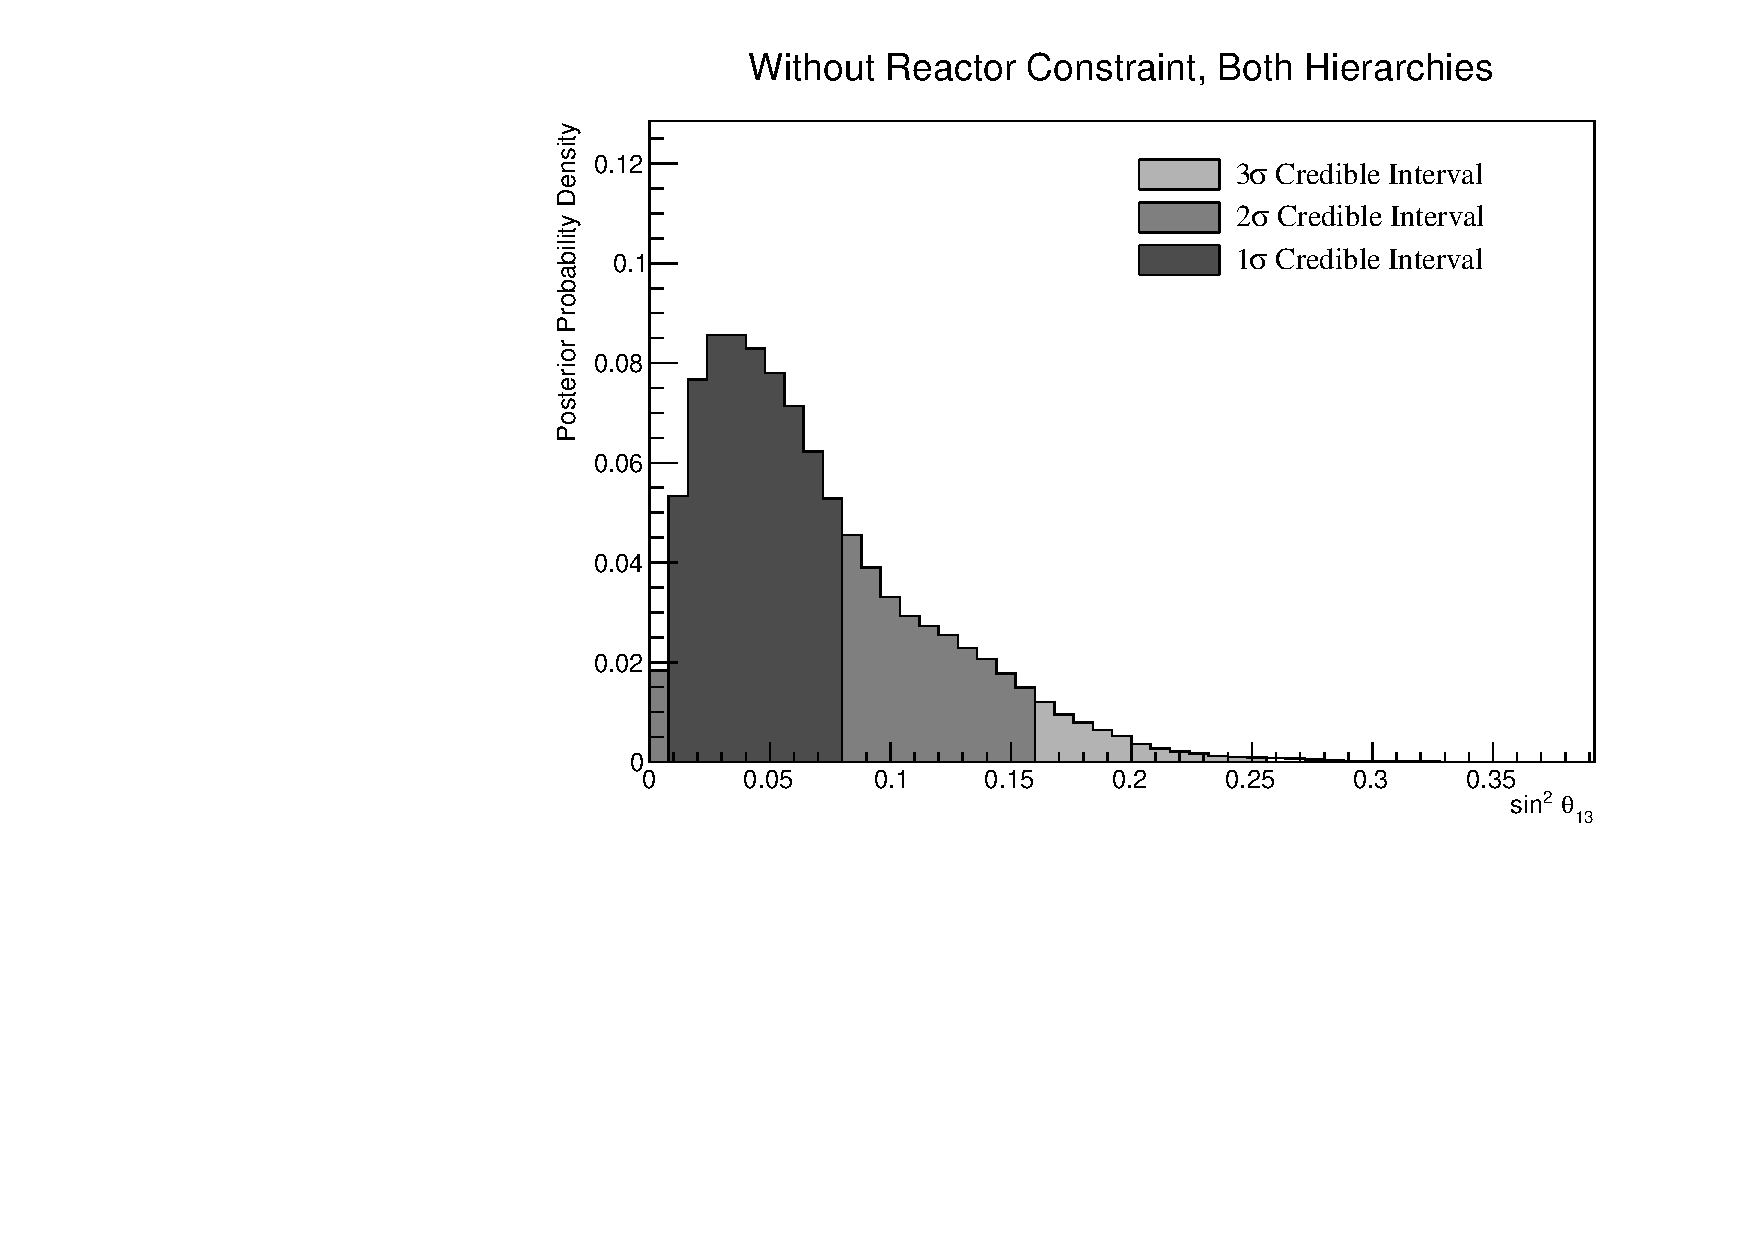
\includegraphics[width=\textwidth, trim={0mm 0mm 0mm 0mm}, clip,page=1]{Figures/OA/SKOnlyFit/Contours_1D_th13_BH_1_woRC_UnSmeared_CredibleInterval.pdf}
  \end{subfigure}
  \caption{The one-dimensional posterior probability density distribution in \quickmath{\sin^{2}(\theta_{13})}, marginalised over both hierarchies, from the SK atmospheric-only fit. The reactor constraint is not applied. The vertical dashed line represents the known value of \quickmath{\sin^{2}(\theta_{13})}.}
  \label{fig:OscillationAnalysis_SKOnly_TH13}
\end{figure}

The sensitivity of the atmospheric samples to \quickmath{\sin^{2}(\theta_{13})} is presented in \autoref{fig:OscillationAnalysis_SKOnly_TH13}. The likelihood scans presented in \autoref{fig:OscillationAnalysis_LLHScanOscPars} suggest that the sensitivity to \quickmath{\sin^{2}(\theta_{13})} will be small. This behaviour is also seen in the fit results, where the width of the \quickmath{1\sigma} credible intervals span the region of \quickmath{\sin^{2}(\theta_{13}) = [0.008, 0.08]}. This is more than an order of magnitude worse than the constraint from reactor experiments \cite{Particle_Data_Group2020-ms}.

\begin{figure}[h]
  \begin{subfigure}[t]{0.98\textwidth}
    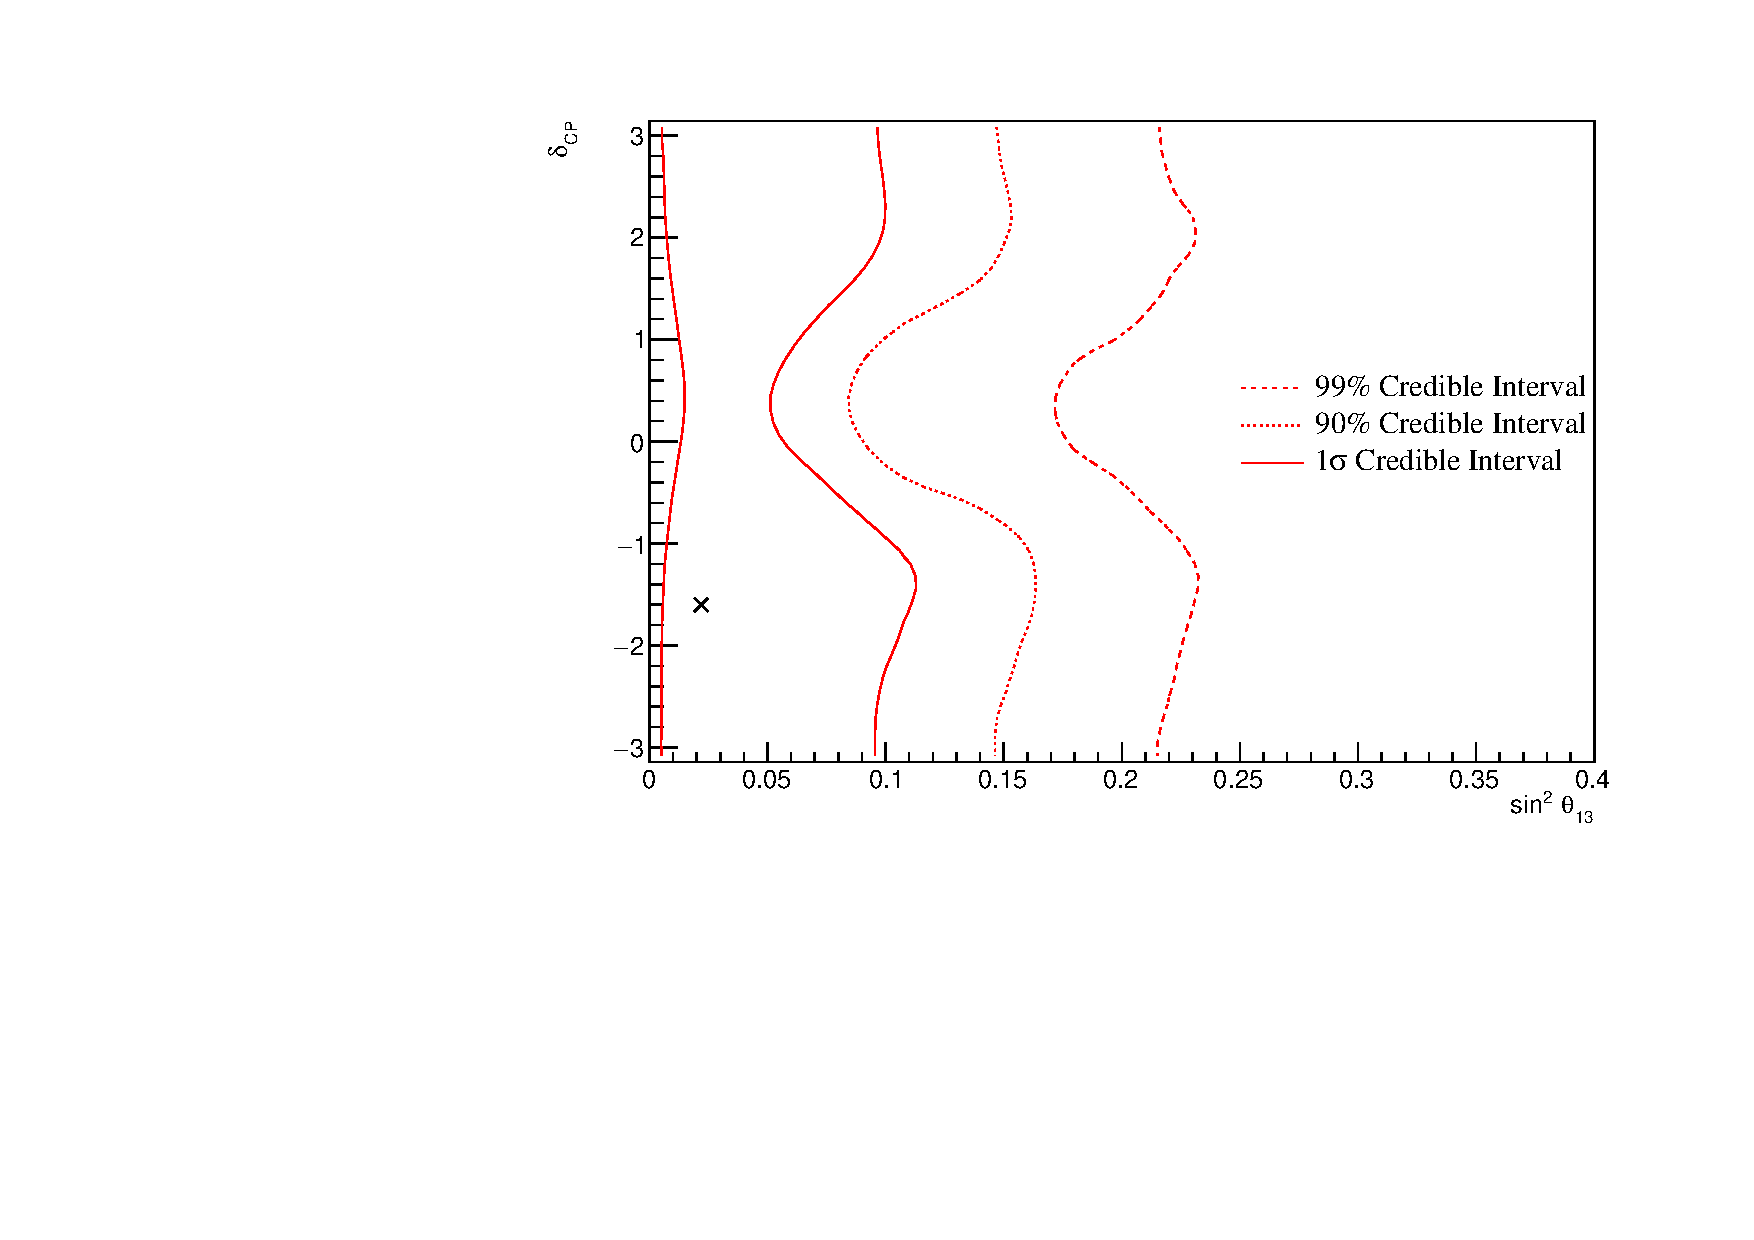
\includegraphics[width=\textwidth, trim={0mm 0mm 0mm 0mm}, clip,page=1]{Figures/OA/SKOnlyFit/Contours_2D_th13_dcp_BH_0_woRC_UnSmeared_CredibleInterval.pdf}
  \end{subfigure}
  \caption{The two-dimensional posterior probability density distribution in \quickmath{\delta_{CP}\text{\textendash}\sin^{2}(\theta_{13})}, marginalised over both hierarchies, from the SK atmospheric-only fit. The reactor constraint is not applied. The marker represents the known value of \quickmath{\delta_{CP}\text{\textendash}\sin^{2}(\theta_{13})}.}
  \label{fig:OscillationAnalysis_SKOnly_DCPTH13}
\end{figure}

As previously discussed, the correlations between oscillation parameters are also important to understand how the atmospheric samples respond. \autoref{fig:OscillationAnalysis_SKOnly_DCPTH13} illustrates the two dimensional \quickmath{\sin^{2}(\theta_{13})\text{\textendash}\delta_{CP}} sensitivity, marginalised over all other parameters.
%The displayed contours are calculated by marginalising over both hierarchies.
The shape of the \quickmath{1\sigma} credible interval shows that the constraining power of the fit on \quickmath{\delta_{CP}} is dependent upon the value of \quickmath{\sin^{2}(\theta_{13})}. Furthermore, they show a strong resemblance to the likelihood scans illustrated in \autoref{fig:OscillationAnalysis_2DLLHOscScans_App}. Whilst the atmospheric samples do not strongly constrain the value of \quickmath{\sin^{2}(\theta_{13})}, the value of \quickmath{\sin^{2}(\theta_{13})} does impact the atmospheric samples' sensitivity to \quickmath{\delta_{CP}}.
%A value of \quickmath{\sin^{2}(\theta_{13}) \sim 0.02} would select a continuous contour over all values of \quickmath{\delta_{CP}}. This shows the effect of the marginalisation effect previously described.

The \quickmath{\sin^{2}(\theta_{23})\text{\textendash}\Delta m^{2}_{32}} disappearance contours are illustrated in \autoref{fig:OscillationAnalysis_SKOnly_DM32TH23}. As expected, the area contained in the inverted hierarchy \quickmath{1\sigma} credible interval is slightly smaller than that in the normal hierarchy. This follows from the Bayes factor showing a weak preference for NH meaning that more of the steps will exist in the \quickmath{\Delta m^{2}_{32} > 0} region. The known oscillation parameters of \quickmath{\sin^{2}(\theta_{23}) = 0.528} and \quickmath{\Delta m^{2}_{32} = 2.509\times 10^{-3}\text{eV}^{2}} are contained within the \quickmath{1\sigma} credible interval.

\begin{figure}[h]
  \begin{subfigure}[t]{0.98\textwidth}
    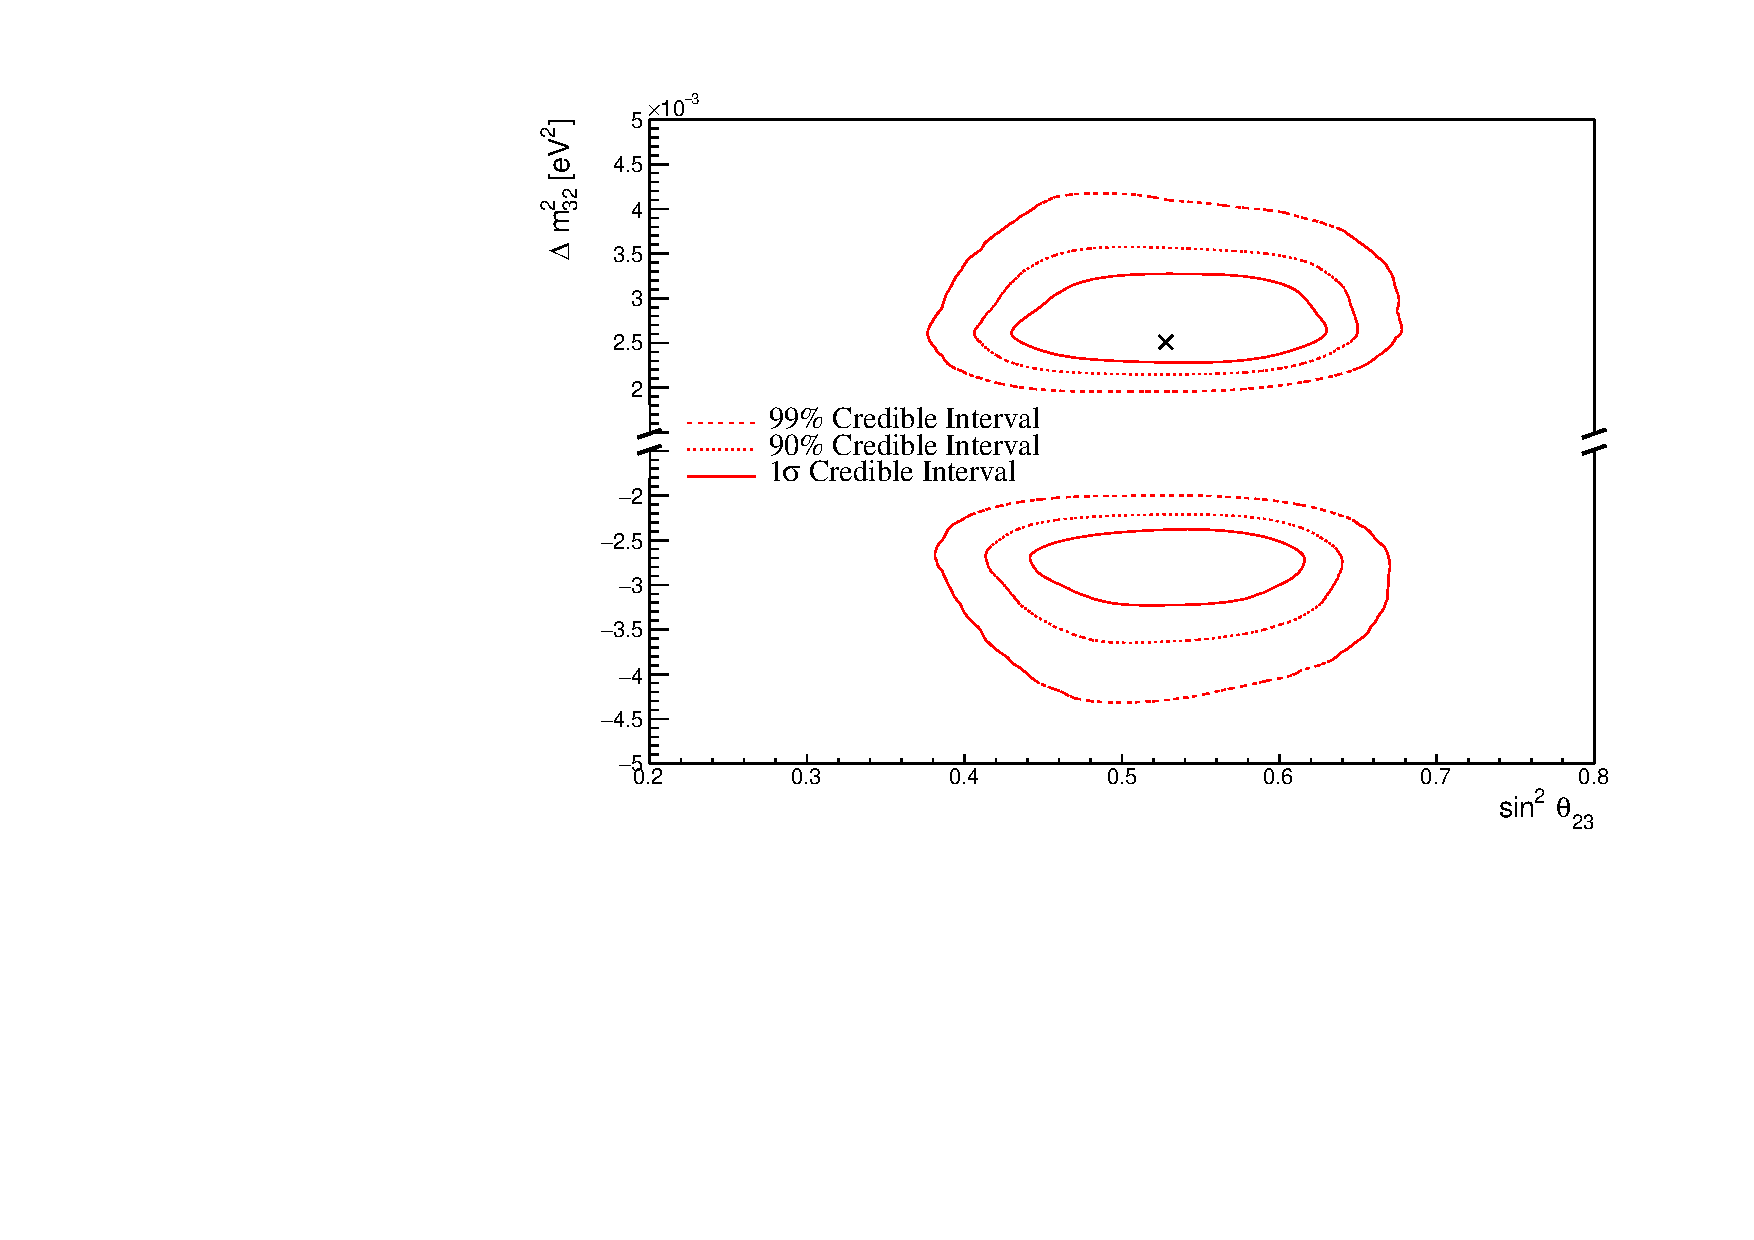
\includegraphics[width=\textwidth, trim={0mm 0mm 0mm 0mm}, clip,page=1]{Figures/OA/SKOnlyFit/Contours_2D_th23_dm32_BH_0_woRC_UnSmeared_CredibleInterval.pdf}
  \end{subfigure}
  \caption{The two-dimensional posterior probability density distribution in \quickmath{\Delta m^{2}_{32}\text{\textendash}\sin^{2}(\theta_{23})}, marginalised over both hierarchies, from the SK atmospheric-only fit. The reactor constraint is not applied. The marker represents the known value of \quickmath{\Delta m^{2}_{32}\text{\textendash}\sin^{2}(\theta_{23})}.}
  \label{fig:OscillationAnalysis_SKOnly_DM32TH23}
\end{figure}

\autoref{fig:OscillationAnalysis_SKOnly_TrianglePlot} illustrates the two-dimensional projections for each permutation of oscillation parameters which this analysis is sensitive to: \quickmath{\delta_{CP}}, \quickmath{\sin^{2}(\theta_{13})}, \quickmath{\sin^{2}(\theta_{23})}, and \quickmath{\Delta m^{2}_{32}}. The purpose of this plot is to illustrate the correlations between the oscillation parameters. The contours are calculated whilst marginalising over both hierarchies, however, only the NH is illustrated when plotting the \quickmath{\Delta m^{2}_{32}} parameter. As expected the correlations play a significant role in these sensitivity measurements, especially the choice of the \quickmath{\sin^{2}(\theta_{13})} constraint. Most notably, the application of reactor constraint would be expected to alter both the width and position of the \quickmath{\Delta m^{2}_{32}} intervals due to the strong correlation between the parameters.

%majority of the octant model preference comes from the region of \quickmath{\sin^{2}(\theta_{13}) \sim 0.03} such that the application of the reactor constraint would not be expected to significantly change the octant preference. The reactor constraint would result in lower values of \quickmath{|\Delta m^{2}_{32}|}.
%Interestingly, the distribution of steps in the \quickmath{\delta_{CP}}\text{\textendash}\quickmath{\sin^{2}(\theta_{13})} plot is slightly flatter in the region of the reactor constraint. Both the posterior distribution from this fit and the distribution in \autoref{fig:OscillationAnalysis_2DLLHOscScans_App} show a region of low negative log-likelihood extending out towards higher values of \quickmath{\sin^{2}(\theta_{13})} in the \quickmath{\delta_{CP} \sim -\pi/2} and \quickmath{\delta_{CP} \sim 2} region. Consequently, the reactor constraint could feasibly reduce the sensitivity of the atmospheric samples to \quickmath{\delta_{CP}}, due to the previously discussed marginalisation effects. 

\begin{figure}[h]
  \begin{subfigure}[t]{0.98\textwidth}
    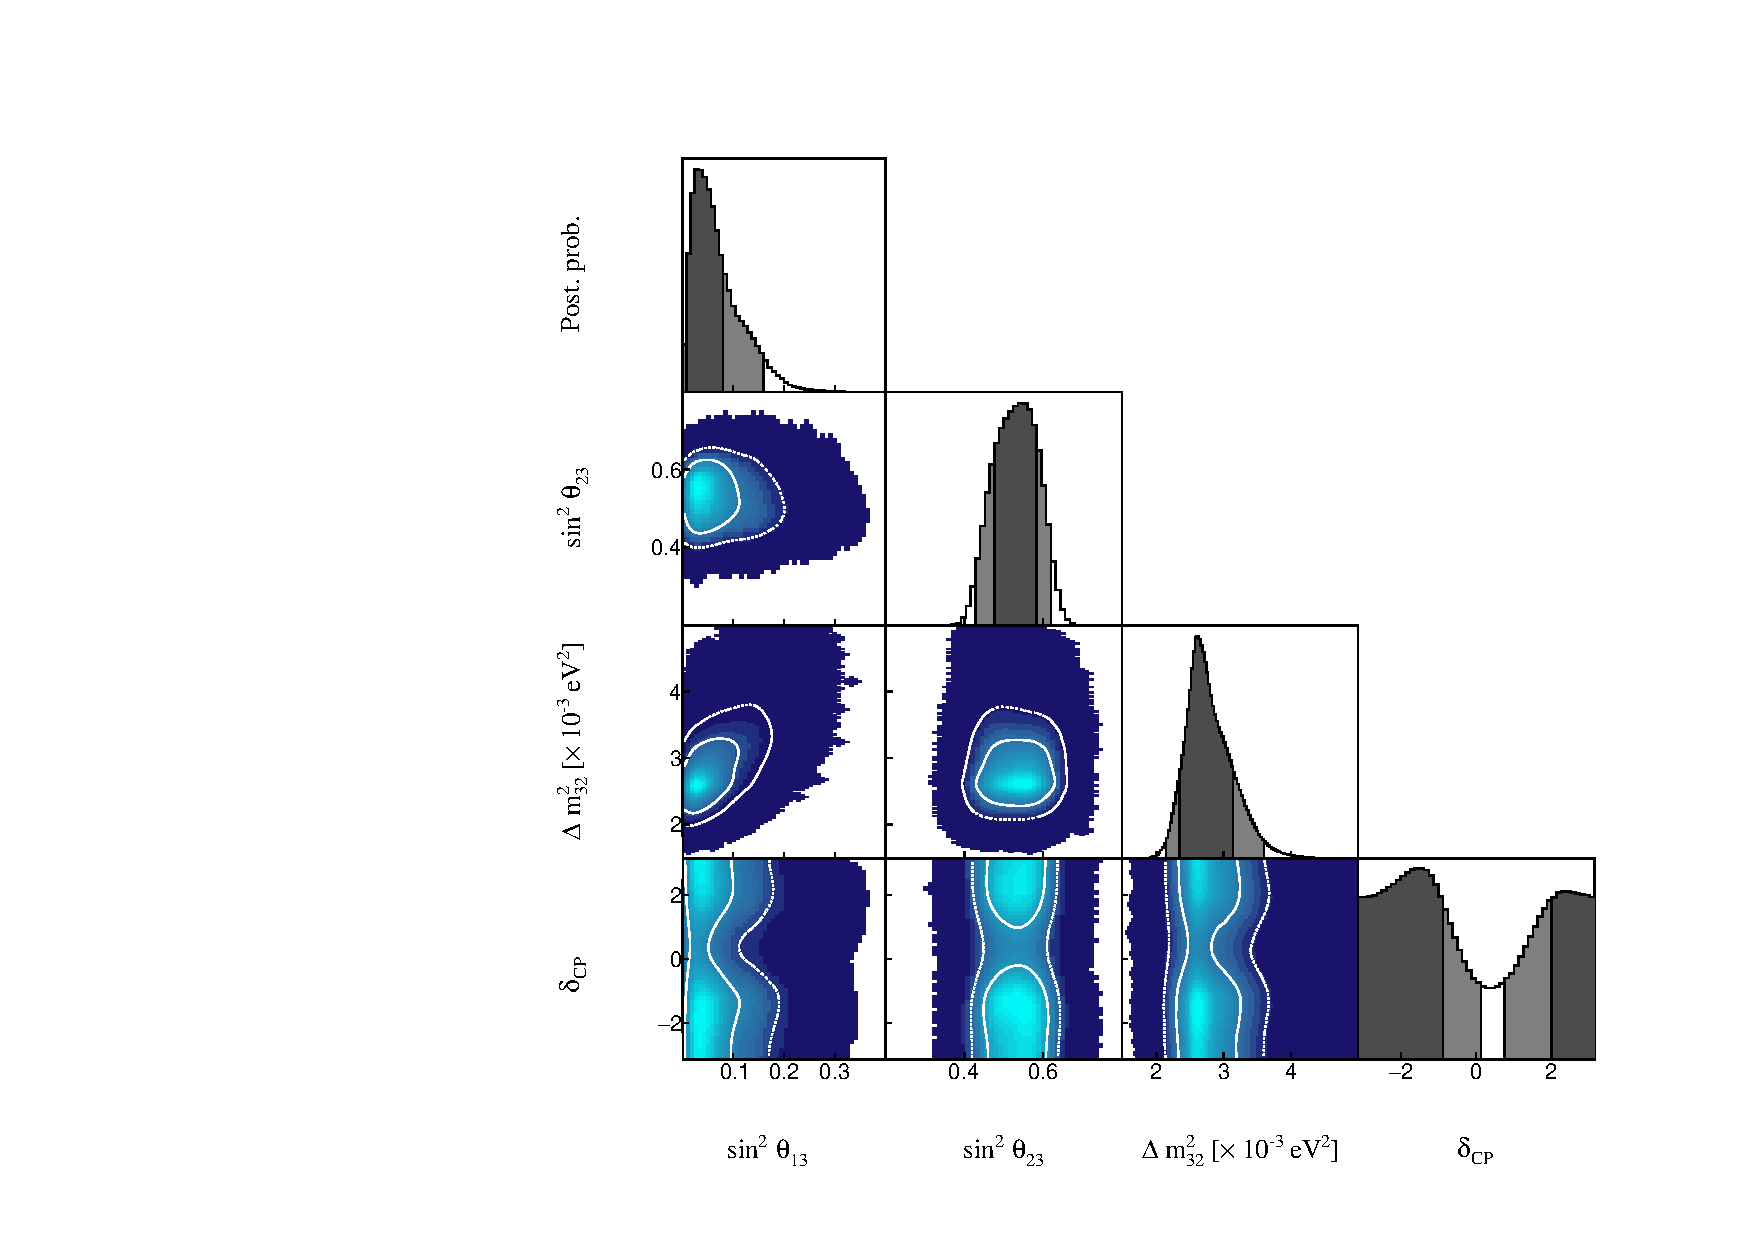
\includegraphics[width=\textwidth, trim={0mm 0mm 0mm 0mm}, clip,page=1]{Figures/OA/SKOnlyFit/Contours_1D_woRC_UnSmeared_CredibleInterval_TrianglePlot.pdf}
  \end{subfigure}
  \caption{The posterior probability density distribution from the SK atmospheric-only fit. The reactor constraint is not applied. The distribution is given for each two-dimensional permutation of the oscillation parameters of interest. The one-dimensional distribution of each parameter is also given.}
  \label{fig:OscillationAnalysis_SKOnly_TrianglePlot}
\end{figure}

\clearpage
\subsection{Atmospheric-Only Sensitivity With Reactor Constraint}
\label{sec:OscillationAnalysis_SKOnly_wRC}

The results in \autoref{sec:OscillationAnalysis_SKOnly} discuss the atmospheric sensitivity when the reactor constraint is not applied. The correlations illustrated in \autoref{fig:OscillationAnalysis_SKOnly_TrianglePlot} indicate that the marginalisation effects could contribute to differing sensitivities when the external reactor constraint is applied. Using the technique discussed in \autoref{sec:MarkovChainMonteCarlo_Priors}, the posterior distribution of the fit in \autoref{sec:OscillationAnalysis_SKOnly} can be reweighted to include the reactor constraint of \quickmath{\sin^{2}(\theta_{13}) = \left(2.18 \pm 0.08 \right) \times 10^{-2}} \cite{Particle_Data_Group2020-ms}.
%The Asimov data is generated assuming the `AsimovA' oscillation parameter set defined in \autoref{tab:Theory_ParameterSets} and the post-BANFF systematic parameter tune.

\iffalse
\begin{figure}[h]
  \begin{subfigure}[t]{0.98\textwidth}
    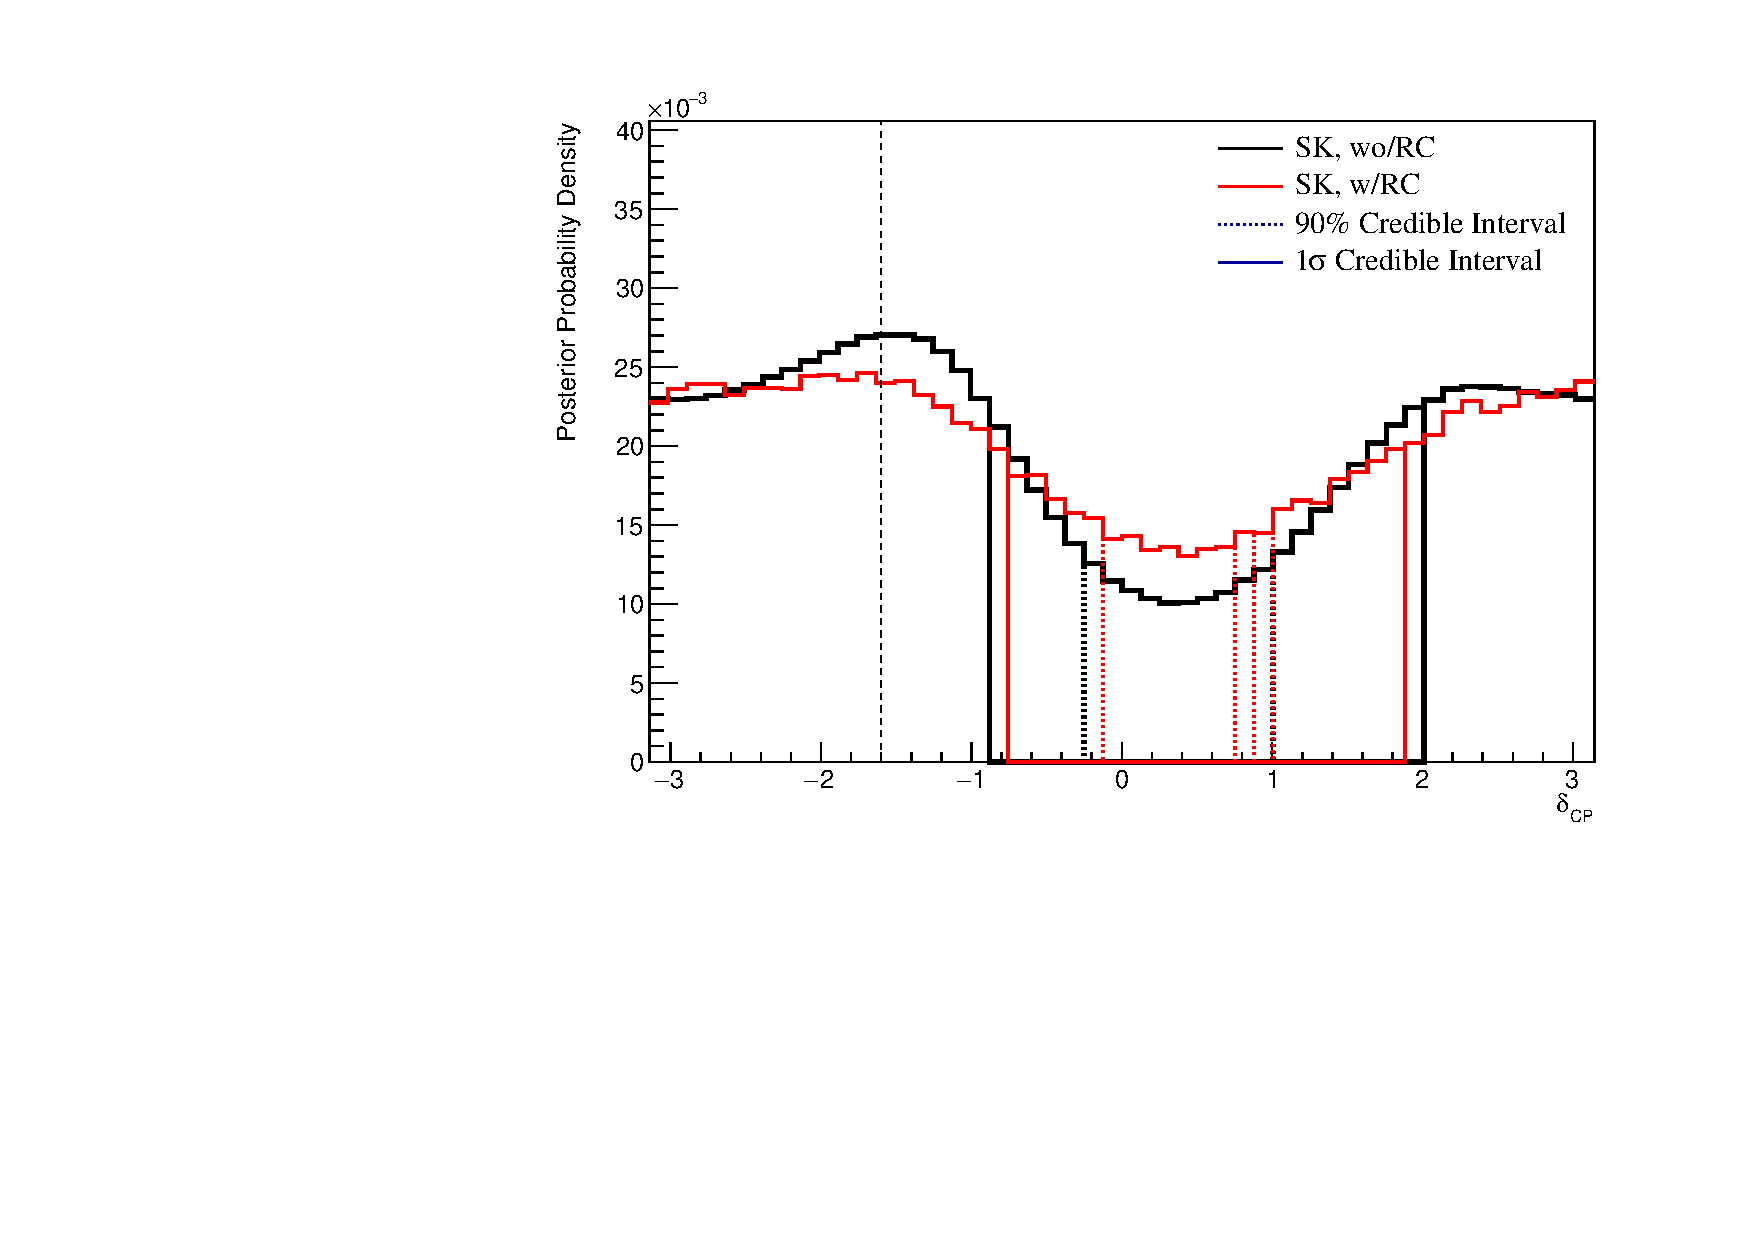
\includegraphics[width=\textwidth, trim={0mm 0mm 0mm 0mm}, clip,page=1]{Figures/OA/SKOnlyFit_wRC/ContourComparison_1D_dcp_BH_2_wRC_woRC_UnSmeared_CredibleInterval.pdf}
  \end{subfigure}
  \caption{The one-dimensional posterior probability density distribution in \quickmath{\delta_{CP}} compared between the SK atmospheric-only fit (Black) and the SK atmospheric fit with the reactor constraint applied (Red). The distributions are marginalised over both hierarchies. The vertical dashed line represents the known value of \quickmath{\delta_{CP}}.}
  \label{fig:OscillationAnalysis_SKOnly_DCP_WRC}
\end{figure}

\autoref{fig:OscillationAnalysis_SKOnly_DCP_WRC} illustrates the sensitivity to \quickmath{\delta_{CP}} of the atmospheric fit with reactor constraint applied. The distribution is less peaked than the previous results. This is due to the expected marginalisation effect previously discussed. The width of the \quickmath{1\sigma} credible interval is increased when the reactor constraint is applied, indicating less sensitivity to \quickmath{\delta_{CP}} in the region of \quickmath{\sin^{2}(\theta_{13})} preferred by the reactor constraint.
\fi

\begin{figure}[h]
  \begin{subfigure}[t]{0.98\textwidth}
    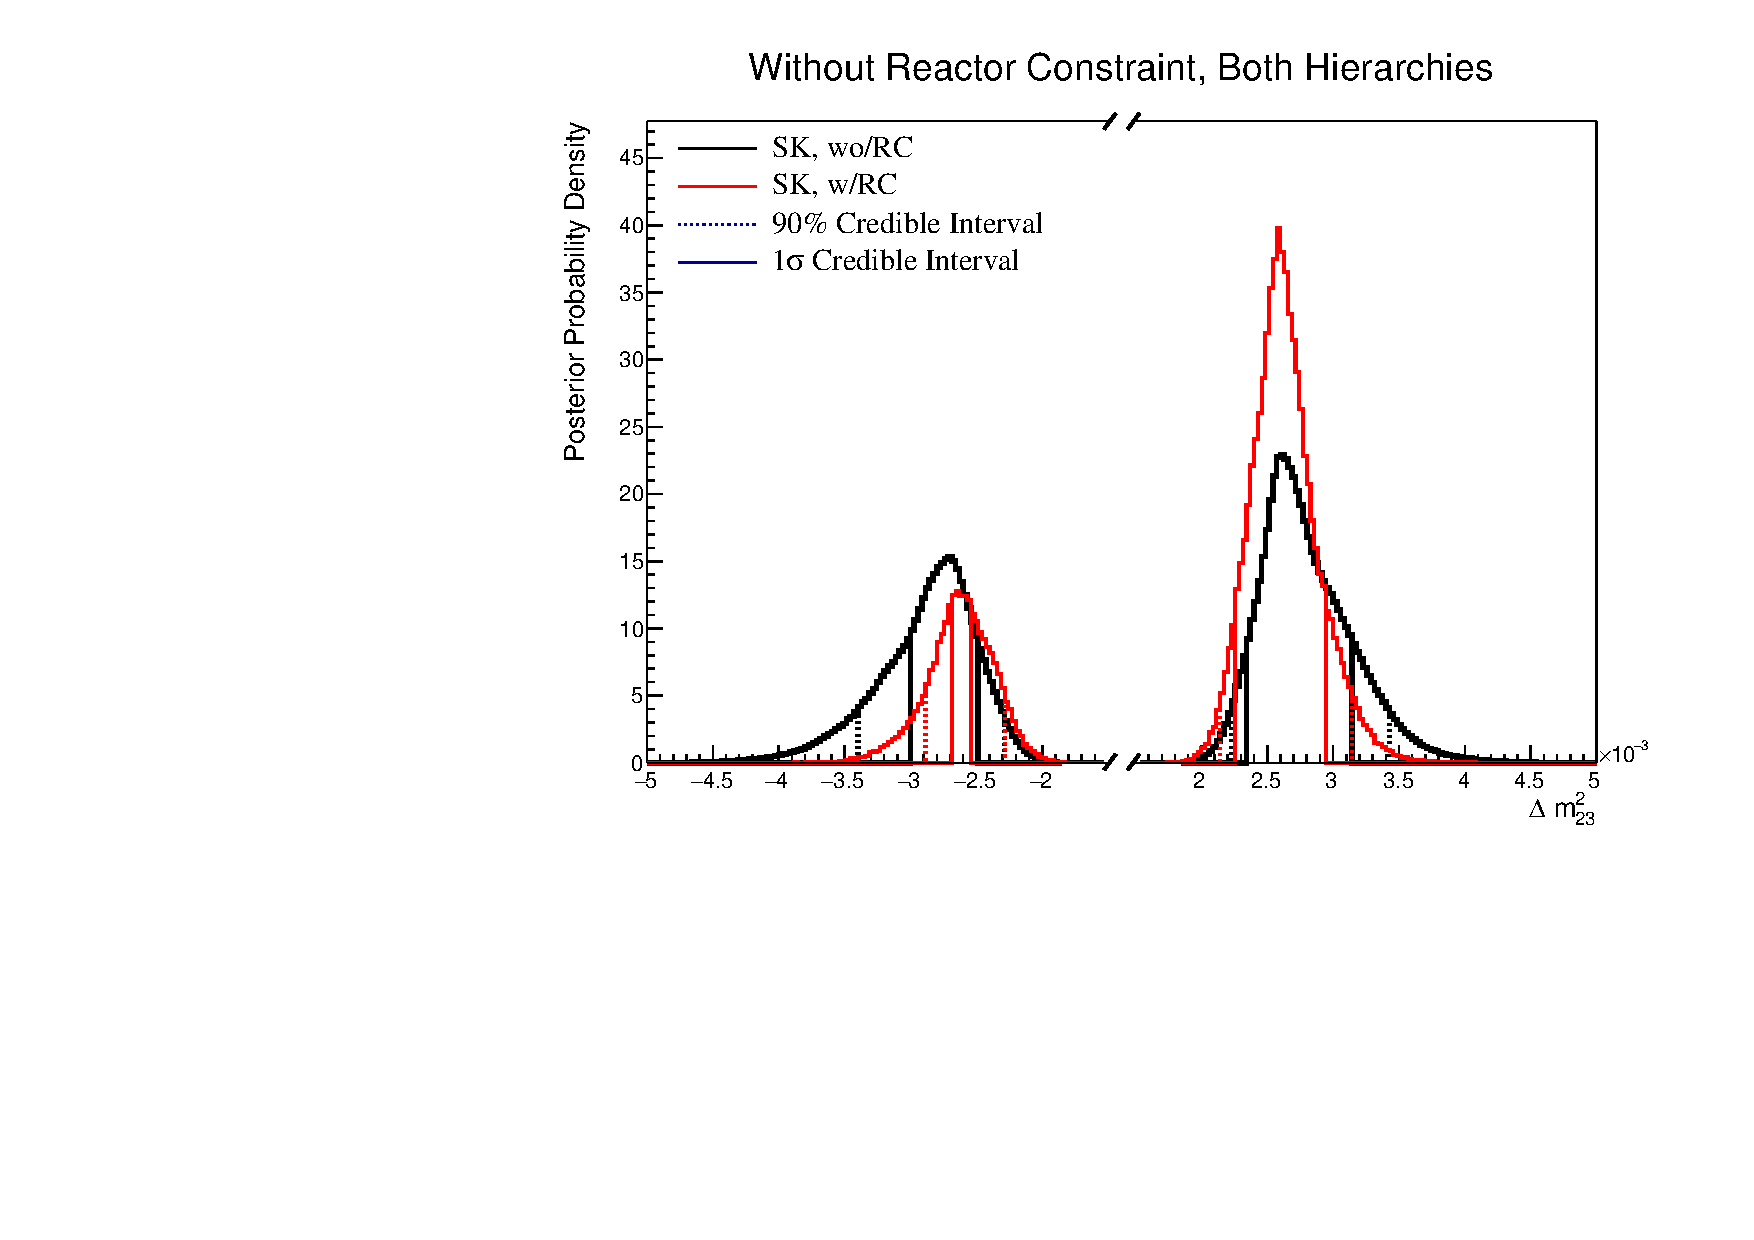
\includegraphics[width=\textwidth, trim={0mm 0mm 0mm 0mm}, clip,page=1]{Figures/OA/SKOnlyFit_wRC/ContourComparison_1D_dm32_BH_2_wRC_woRC_UnSmeared_CredibleInterval.pdf}
  \end{subfigure}
  \caption{The one-dimensional posterior probability density distribution in \quickmath{\Delta m^{2}_{32}} compared between the SK atmospheric-only fit (Black) and the SK atmospheric fit with the reactor constraint applied (Red). The distributions are marginalised over both hierarchies. The vertical dashed line represents the known value of \quickmath{\Delta m^{2}_{32}}.}
  \label{fig:OscillationAnalysis_SKOnly_DELM32_WRC}
\end{figure}

The reactor constraint increases the sensitivity of the atmospheric samples to \quickmath{\Delta m^{2}_{32}} as illustrated in \autoref{fig:OscillationAnalysis_SKOnly_DELM32_WRC}. The \quickmath{1\sigma} credible interval in \quickmath{\Delta m^{2}_{32}} is determined to be \quickmath{[-2.69, -2.54] \times 10^{-3} \text{eV}^{2}} and \quickmath{[2.25, 2.94] \times 10^{-3} \text{eV}^{2}}. The width of the IH credible interval is reduced by \quickmath{\sim70\%} when the reactor constraint is applied. Due to the marginalisation effects observed in \autoref{fig:OscillationAnalysis_SKOnly_TrianglePlot}, the favoured region of \quickmath{\Delta m^{2}_{32}} moves closer to zero for both hierarchies. A clear explanation of this behaviour is illustrated in \autoref{fig:OscillationAnalysis_SKOnly_DELM32TH13_WRC}, which shows the posterior distribution in the \quickmath{\Delta m^{2}_{32}-\sin^{2}(\theta_{13})} parameters. The correlation between \quickmath{\Delta m^{2}_{32}} and \quickmath{\sin^{2}(\theta_{13})} is such that lower values of \quickmath{\sin^{2}(\theta_{13})} tend towards lower values of \quickmath{|\Delta m^{2}_{32}|}. Therefore the application of the reactor constraint moves the posterior distribution towards the known oscillation parameter.
%\quickmath{\Delta m^{2}_{32} = 2.509 \times 10^{-3} \text{eV}^{2}}.

\begin{figure}[h]
  \begin{subfigure}[t]{0.98\textwidth}
    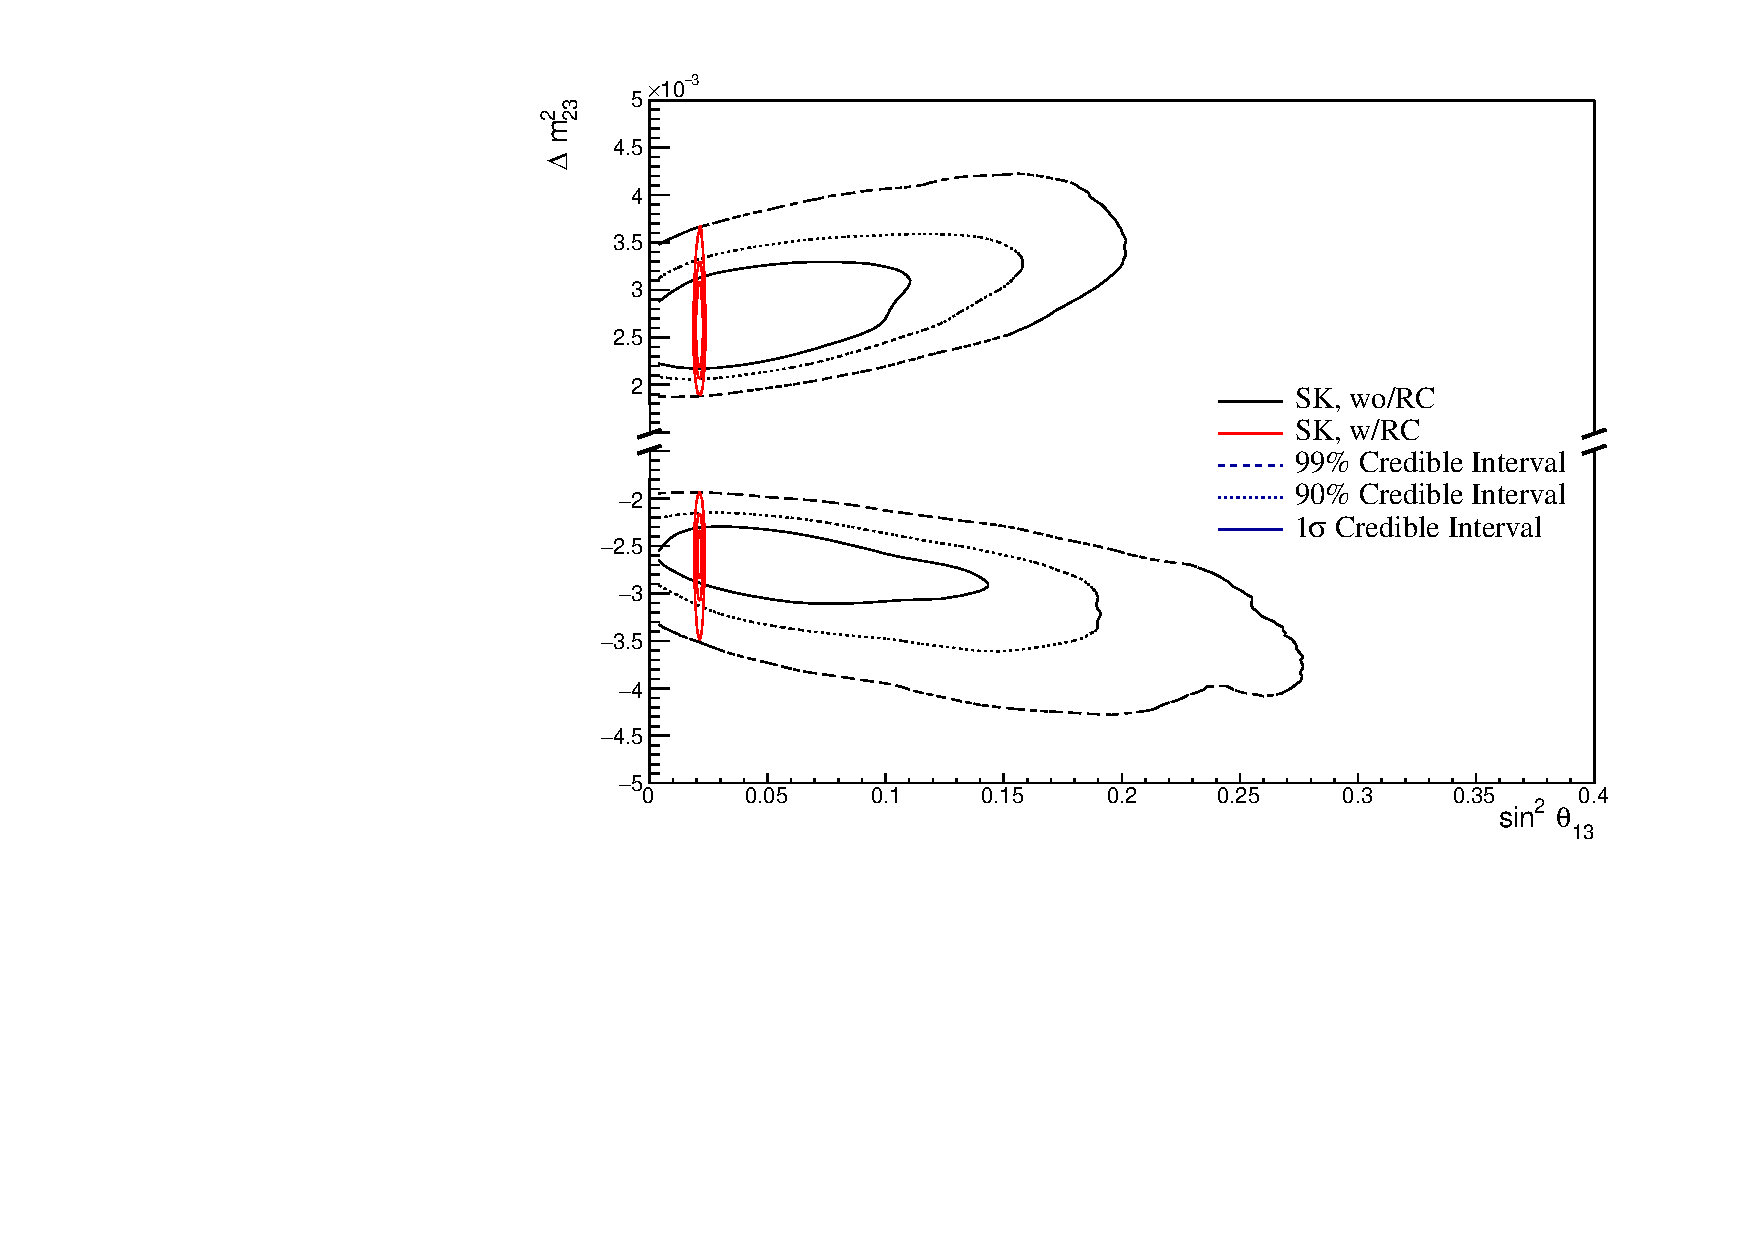
\includegraphics[width=\textwidth, trim={0mm 0mm 0mm 0mm}, clip,page=1]{Figures/OA/SKOnlyFit_wRC/ContourComparison_2D_th13_dm32_BH_0_wRC_woRC_UnSmeared_CredibleInterval.pdf}
  \end{subfigure}
    \caption{The two-dimensional posterior probability density distribution in \quickmath{\Delta m^{2}_{32}\text{\textendash}\sin^{2}(\theta_{13})} compared between the SK atmospheric-only fit (Black) and the SK atmospheric fit with the reactor constraint (Red). The distributions are marginalised over both hierarchies. The marker represents the known value of \quickmath{\Delta m^{2}_{32}\text{\textendash}\sin^{2}(\theta_{13})}.}
  \label{fig:OscillationAnalysis_SKOnly_DELM32TH13_WRC}
\end{figure}

\begin{table}[ht!]
  \centering
  \begingroup
  \renewcommand{\arraystretch}{1.5}
  \begin{tabular}{c|cc|c}
                                                        & LO \quickmath{\left(\sin^{2}\theta_{23} < 0.5 \right)} & UO \quickmath{\left( \sin^{2}\theta_{23} > 0.5 \right)} & Sum  \\ \hline
    NH \quickmath{\left( \Delta m^{2}_{32} > 0 \right)} &                                                   0.21 &                                                    0.53 & 0.74 \\
    IH \quickmath{\left( \Delta m^{2}_{32} < 0 \right)} &                                                   0.08 &                                                    0.18 & 0.26 \\ \hline
    Sum                                                 &                                                   0.29 &                                                    0.71 & 1.00 \\
  \end{tabular}
  \caption{The distribution of steps in an SK atmospheric with reactor constraint fit, presented as the fraction of steps in the upper (UO) and lower (LO) octants and the normal (NH) and inverted (IH) hierarchies. The Bayes factors are calculated as \quickmath{B(\text{NH}/\text{IH}) = 2.85} and \quickmath{B(\text{UO}/\text{LO}) = 2.39}.}
  \label{tab:OscillationAnalysis_SKOnlyWRC_BayesFactors}
  \endgroup
\end{table}


\autoref{tab:OscillationAnalysis_SKOnlyWRC_BayesFactors} presents the fraction of steps in each hierarchy and octant model for the fit after the reactor constraint has been applied. The reactor constraint significantly increases the preference for the correct hierarchy, increasing the Bayes factor from \quickmath{B(\text{NH}/\text{IH}) = 1.37} to \quickmath{B(\text{NH}/\text{IH}) = 2.85} when the reactor constraint is applied. This is still defined as a weak preference for the NH hypothesis according to Jeffrey's scale, however, it is a stronger preference than when the constraint is not applied. The preference for the correct octant model is also slightly increased by the application of the reactor constraint.

%The asymmetry in the number of steps within the NH to IH shows that the reactor constraint increases preference for the NH hypothesis. The fraction of steps in each hierarchy and octant model for this fit are given in \autoref{tab:OscillationAnalysis_SKOnlyWRC_BayesFactors}. The preference for the correct octant model is very slightly increased by the application of the reactor constraint which is consistent with expectation. The reactor constraint significantly increases the NH preference, increasing the Bayes factor from \quickmath{B(\text{NH}/\text{IH}) = 1.37} to \quickmath{B(\text{NH}/\text{IH}) = 2.86} when the reactor constraint is applied. This is still defined as a weak preference for NH according to Jeffrey's scale (see \autoref{tab:MarkovChainMonteCarlo_JeffreysScale}), however, it is a stronger preference than without the constraint. The Bayes factor for octant determination is calculated as \quickmath{B(\text{UO}/\text{LO}) = 2.39}.

\clearpage
\subsection{Impact of Near Detector Constraints for Atmospheric Samples}
\label{sec:OscillationAnalysis_SKOnly_NoND}

The choice of applying the near detector constraints to the low-energy atmospheric samples was introduced in \autoref{sec:SelsAndSysts_Systs_Interaction}. This subsection illustrates the effect of removing the ND constraint on the sensitivity of the atmospheric samples to the oscillation parameters. To do this, the fit presented in \autoref{sec:OscillationAnalysis_SKOnly} has been compared to another fit where the constraints from the near detector have not been included.
%In practice, this alternative fit does not consider any near detector samples when fitting the atmospheric samples.
This is the only case where the near detector constraints are neglected throughout this chapter. For both fits, the Asimov data was generated assuming the `AsimovA' oscillation parameter set defined in \autoref{tab:Theory_ParameterSets} and the post-BANFF systematic parameter tune.

The change in sensitivity on \quickmath{\delta_{CP}} is given in \autoref{fig:OscillationAnalysis_SKOnly_NoND_DCP}. The reactor constraint is not applied in either of the fits within this comparison. The fit which includes the near detector constraint is slightly more peaked at the known oscillation parameter value. The width of the \quickmath{1\sigma} credible intervals are approximately the same (identical to within a bin width) and the same conclusion holds for the higher credible intervals. The change in sensitivity to other oscillation parameters has been studied and no significant discrepancies were found. This shows that the exact choice of constraint does not significantly affect the physics conclusions one would make from this analysis.

\begin{figure}[h]
  \begin{subfigure}[t]{0.98\textwidth}
    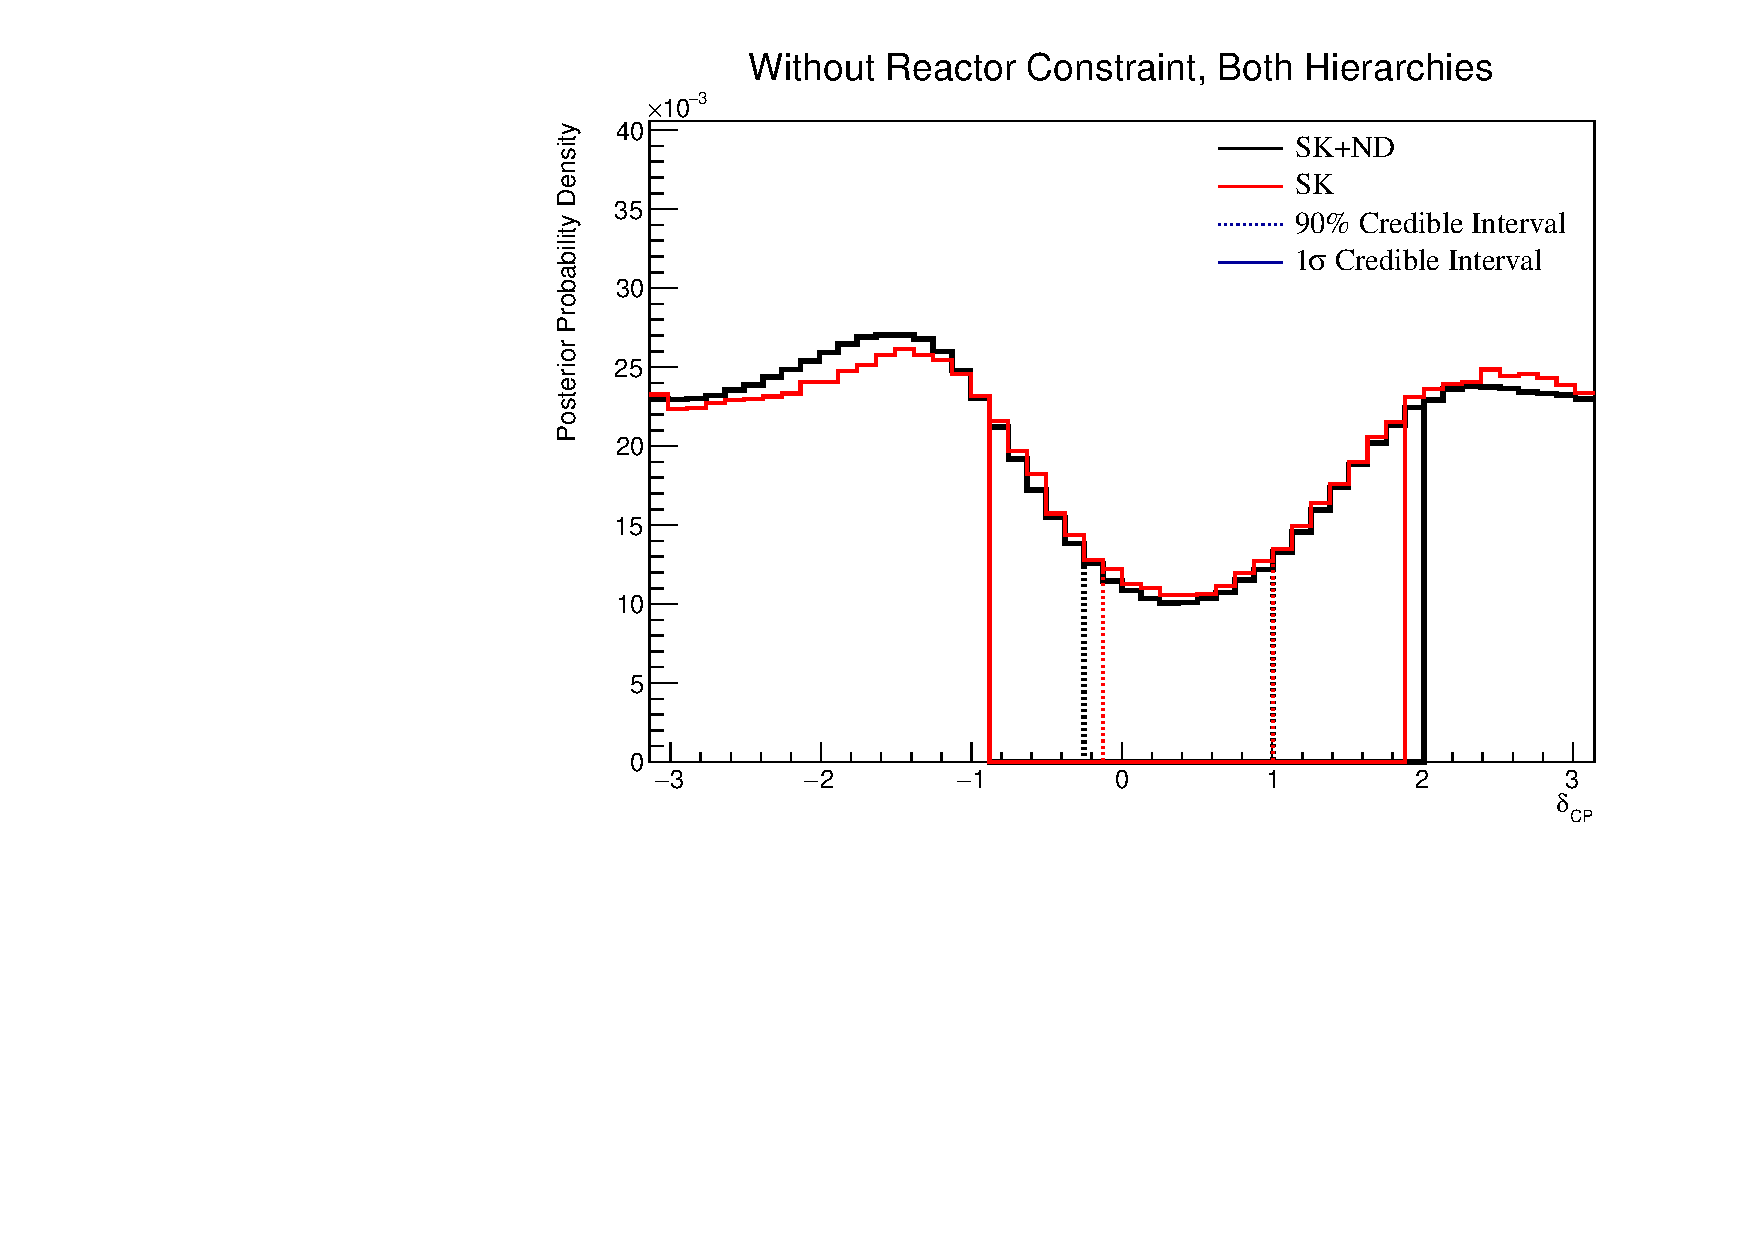
\includegraphics[width=\textwidth, trim={0mm 0mm 0mm 0mm}, clip,page=1]{Figures/OA/SKOnlyFit_noND/ContourComparison_1D_dcp_BH_2_woRC_UnSmeared_CredibleInterval.pdf}
  \end{subfigure}
  \caption{The one-dimensional posterior probability density distribution in \quickmath{\delta_{CP}} compared between the SK atmospheric-only fit where the near detector constraint is (Black) and is not (Red) applied. The distributions are marginalised over both hierarchies. The reactor constraint is not applied in either fit. The vertical dashed line represents the known value of \quickmath{\delta_{CP}}.}
  \label{fig:OscillationAnalysis_SKOnly_NoND_DCP}
\end{figure}

\clearpage
\subsection{Atmospheric and Beam Sensitivity without Reactor Constraint}
\label{sec:OscillationAnalysis_JointFit}

This section presents the sensitivities of the simultaneous beam and atmospheric analysis where the reactor constraint is not applied. Similar to the previous studies, the Asimov data is built assuming the post-BANFF systematic tune and Asimov A oscillation parameters defined in \autoref{tab:Theory_ParameterSets}. This fit uses all 18 near detector beam samples, 5 far detector beam samples, and 18 atmospheric samples. 

\begin{figure}[h]
  \begin{subfigure}[t]{0.98\textwidth}
    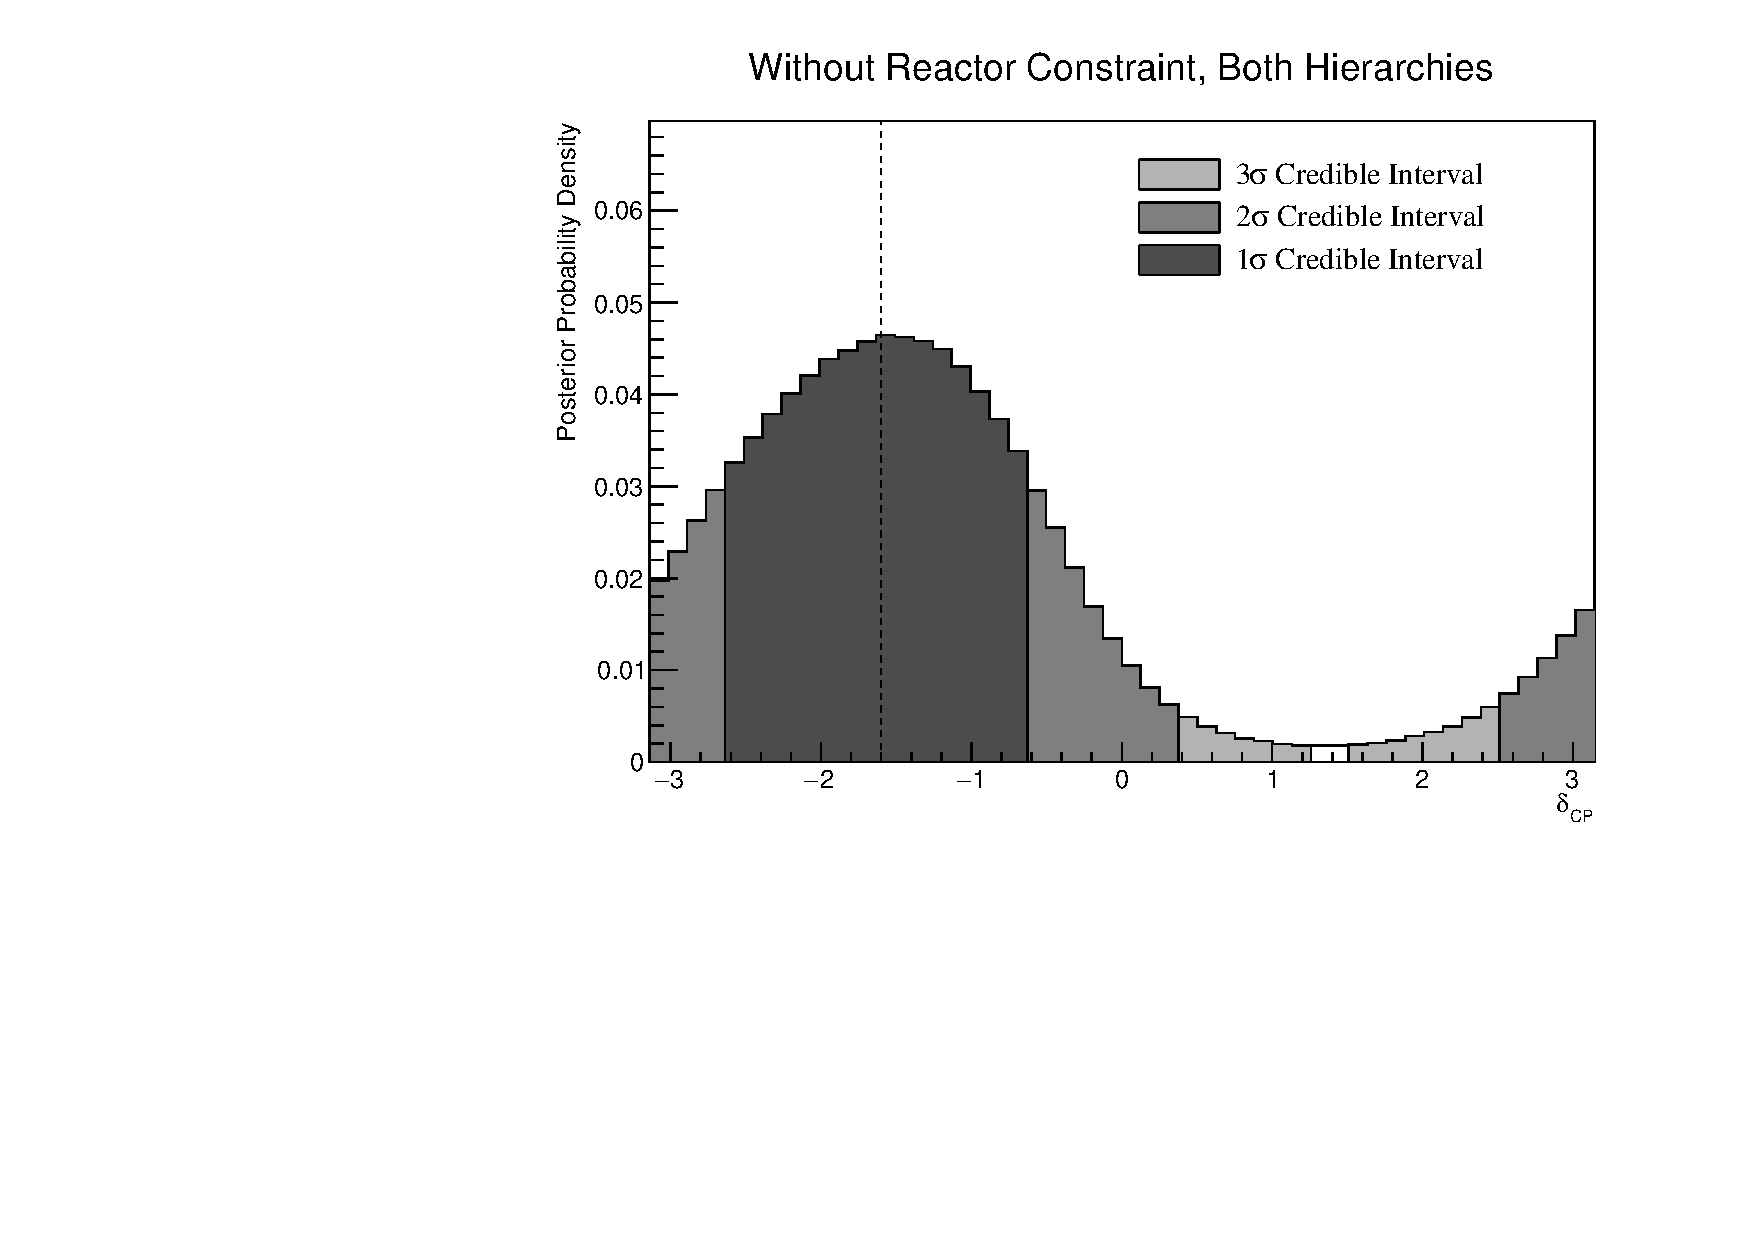
\includegraphics[width=\textwidth, trim={0mm 0mm 0mm 0mm}, clip,page=1]{Figures/OA/JointFit/Contours_1D_dcp_BH_1_woRC_UnSmeared_CredibleInterval.pdf}
  \end{subfigure}
  \caption{The one-dimensional posterior probability density distribution in \quickmath{\delta_{CP}}, marginalised over both hierarchies, from the joint beam-atmospheric fit. The reactor constraint is not applied. The vertical dashed line represents the known value of \quickmath{\delta_{CP}}.}
  \label{fig:OscillationAnalysis_JointFit_DCP}
\end{figure}

The sensitivity to \quickmath{\delta_{CP}}, marginalised over both hierarchies, is given in \autoref{fig:OscillationAnalysis_JointFit_DCP}. The credible intervals and highest posterior distribution for each oscillation parameter is given in \autoref{tab:OscillationAnalysis_JointFit_CredIntervals}. The highest posterior probability density is \quickmath{\delta_{CP} = -1.57 \pm 0.07} and is compatible with the known value of \quickmath{\delta_{CP} = -1.601}. The CP-conserving values of \quickmath{\delta_{CP}=0, \pm\pi} are disfavoured at \quickmath{1\sigma} credible interval. There is also a region around \quickmath{\delta_{CP} = 1.4} which is disfavoured at more than \quickmath{3\sigma}. Whilst these conclusions can only be made at this particular Asimov point, it does show that if the true value of \quickmath{\delta_{CP}} were CP-violating, this joint analysis would be able to disfavour CP conserving values at over \quickmath{1\sigma} without any external constraints.
%The highest posterior probability density does move further away from the Asimov point when only steps in the NH region are considered. This is due to the correlations between the value of \quickmath{\delta_{CP}} and the mass hierarchy, as will be later discussed.

\begin{table}[ht!]
  \centering
  \begingroup
  \renewcommand{\arraystretch}{1.5}
  \begin{tabular}{c|c|c}
    Parameter               & Interval & HPD \\ \hline
    \quickmath{\delta_{CP}, \text{ (BH)}} & \quickmath{\left[ -2.64, -0.63 \right]} & \quickmath{-1.57 \pm 0.07} \\
    \quickmath{\delta_{CP}, \text{ (NH)}} & \quickmath{\left[ -2.76, -0.63 \right]} & \quickmath{-1.45 \pm 0.07} \\
    \quickmath{\delta_{CP}, \text{ (IH)}} & \quickmath{\left[ -2.39, -0.88 \right]} & \quickmath{-1.57 \pm 0.07} \\ \hline
    \quickmath{\Delta m^{2}_{32} \text{ (BH) } [\times 10^{-3} \text{eV}^{2}]} & \quickmath{\left[ 2.45, 2.58 \right]} & \quickmath{2.51 \pm 0.01} \\
    \quickmath{\Delta m^{2}_{32} \text{ (NH) } [\times 10^{-3} \text{eV}^{2}]} & \quickmath{\left[ 2.47, 2.56 \right]} & \quickmath{2.51 \pm 0.01} \\
    \quickmath{\Delta m^{2}_{32} \text{ (IH) } [\times 10^{-3} \text{eV}^{2}]} & \quickmath{\left[ -2.60, -2.51 \right]} & \quickmath{-2.55 \pm 0.01} \\ \hline
    \quickmath{\sin^{2}(\theta_{23}) \text{ (BH) }} & \quickmath{\left[ 0.480, 0.545 \right]} & \quickmath{0.518 \pm 0.003} \\ 
    \quickmath{\sin^{2}(\theta_{23}) \text{ (NH) }} & \quickmath{\left[ 0.480, 0.545 \right]} & \quickmath{0.508 \pm 0.003} \\ 
    \quickmath{\sin^{2}(\theta_{23}) \text{ (IH) }} & \quickmath{\left[ 0.480, 0.545 \right]} & \quickmath{0.513 \pm 0.003} \\ \hline \hline
  \end{tabular}
  \caption{The position of the highest posterior probability density (HPD) and width of the \quickmath{1\sigma} credible interval for the joint beam-atmospheric fit. The reactor constraint is not applied. The values are presented by which hierarchy hypothesis is assumed: marginalised over both hierarchies (BH), normal hierarchy only (NH), and inverted hierarchy only (IH).}
  \label{tab:OscillationAnalysis_JointFit_CredIntervals}
  \endgroup
\end{table}

The sensitivity to \quickmath{\Delta m^{2}_{32}} is illustrated in \autoref{fig:OscillationAnalysis_JointFit_DELM32}. Notably, the \quickmath{1\sigma} credible interval is entirely contained within the NH region, as further evidenced by \autoref{tab:OscillationAnalysis_JointFit_CredIntervals}. This illustrates good sensitivity to the mass hierarchy as it is correctly selecting the correct hypothesis. This is reflected in the \quickmath{1\sigma} credible intervals being approximately the same when they are constructed considering both hierarchies and when considering only the NH region. The NH distribution favours this region surrounding the known Asimov point, \quickmath{\Delta m^{2}_{32} = 2.509 \times 10 ^{-3} \text{eV}^{2}}, where the highest posterior probability density is at \quickmath{\Delta m^{2}_{32} = (2.51 \pm 0.01) \times 10 ^{-3} \text{eV}^{2}}. 

The fraction of steps in each of the mass hierarchy regions and octants of \quickmath{\sin^{2}(\theta_{23})} is given in \autoref{tab:OscillationAnalysis_JointFit_BayesFactors}. The Bayes factors are determined to be \quickmath{B(\text{NH}/\text{IH}) = 3.67} and \quickmath{B(\text{UO}/\text{LO}) = 1.74}. Jeffrey's scale states that this value of the mass hierarchy Bayes factor illustrates substantial evidence for the NH hypothesis. This corresponds to the correct hypothesis given the known oscillation parameters and is a stronger statement than the atmospheric-only analysis can provide. It is important to note that this substantial preference requires no external constraints. The Bayes factor for octant determination represents a weak preference for the upper octant, therefore, selecting the correct octant hypothesis.

\begin{table}[ht!]
  \centering
  \begingroup
  \renewcommand{\arraystretch}{1.5}
  \begin{tabular}{c|cc|c}
                                                        & LO \quickmath{\left(\sin^{2}\theta_{23} < 0.5 \right)} & UO \quickmath{\left( \sin^{2}\theta_{23} > 0.5 \right)} & Sum  \\ \hline
    NH \quickmath{\left( \Delta m^{2}_{32} > 0 \right)} &                                                   0.29 &                                                    0.50 & 0.79 \\
    IH \quickmath{\left( \Delta m^{2}_{32} < 0 \right)} &                                                   0.08 &                                                    0.13 & 0.21 \\ \hline
    Sum                                                 &                                                   0.37 &                                                    0.63 & 1.00 \\
  \end{tabular}
  \caption{The distribution of steps in a joint beam-atmospheric fit, presented as the fraction of steps in the upper (UO) and lower (LO) octants and the normal (NH) and inverted (IH) hierarchies. The reactor constraint is not applied. The Bayes factors are calculated as \quickmath{B(\text{NH}/\text{IH}) = 3.67} and \quickmath{B(\text{UO}/\text{LO}) = 1.74}.}
  \label{tab:OscillationAnalysis_JointFit_BayesFactors}
  \endgroup
\end{table}

\begin{figure}[h]
  \begin{subfigure}[t]{0.98\textwidth}
    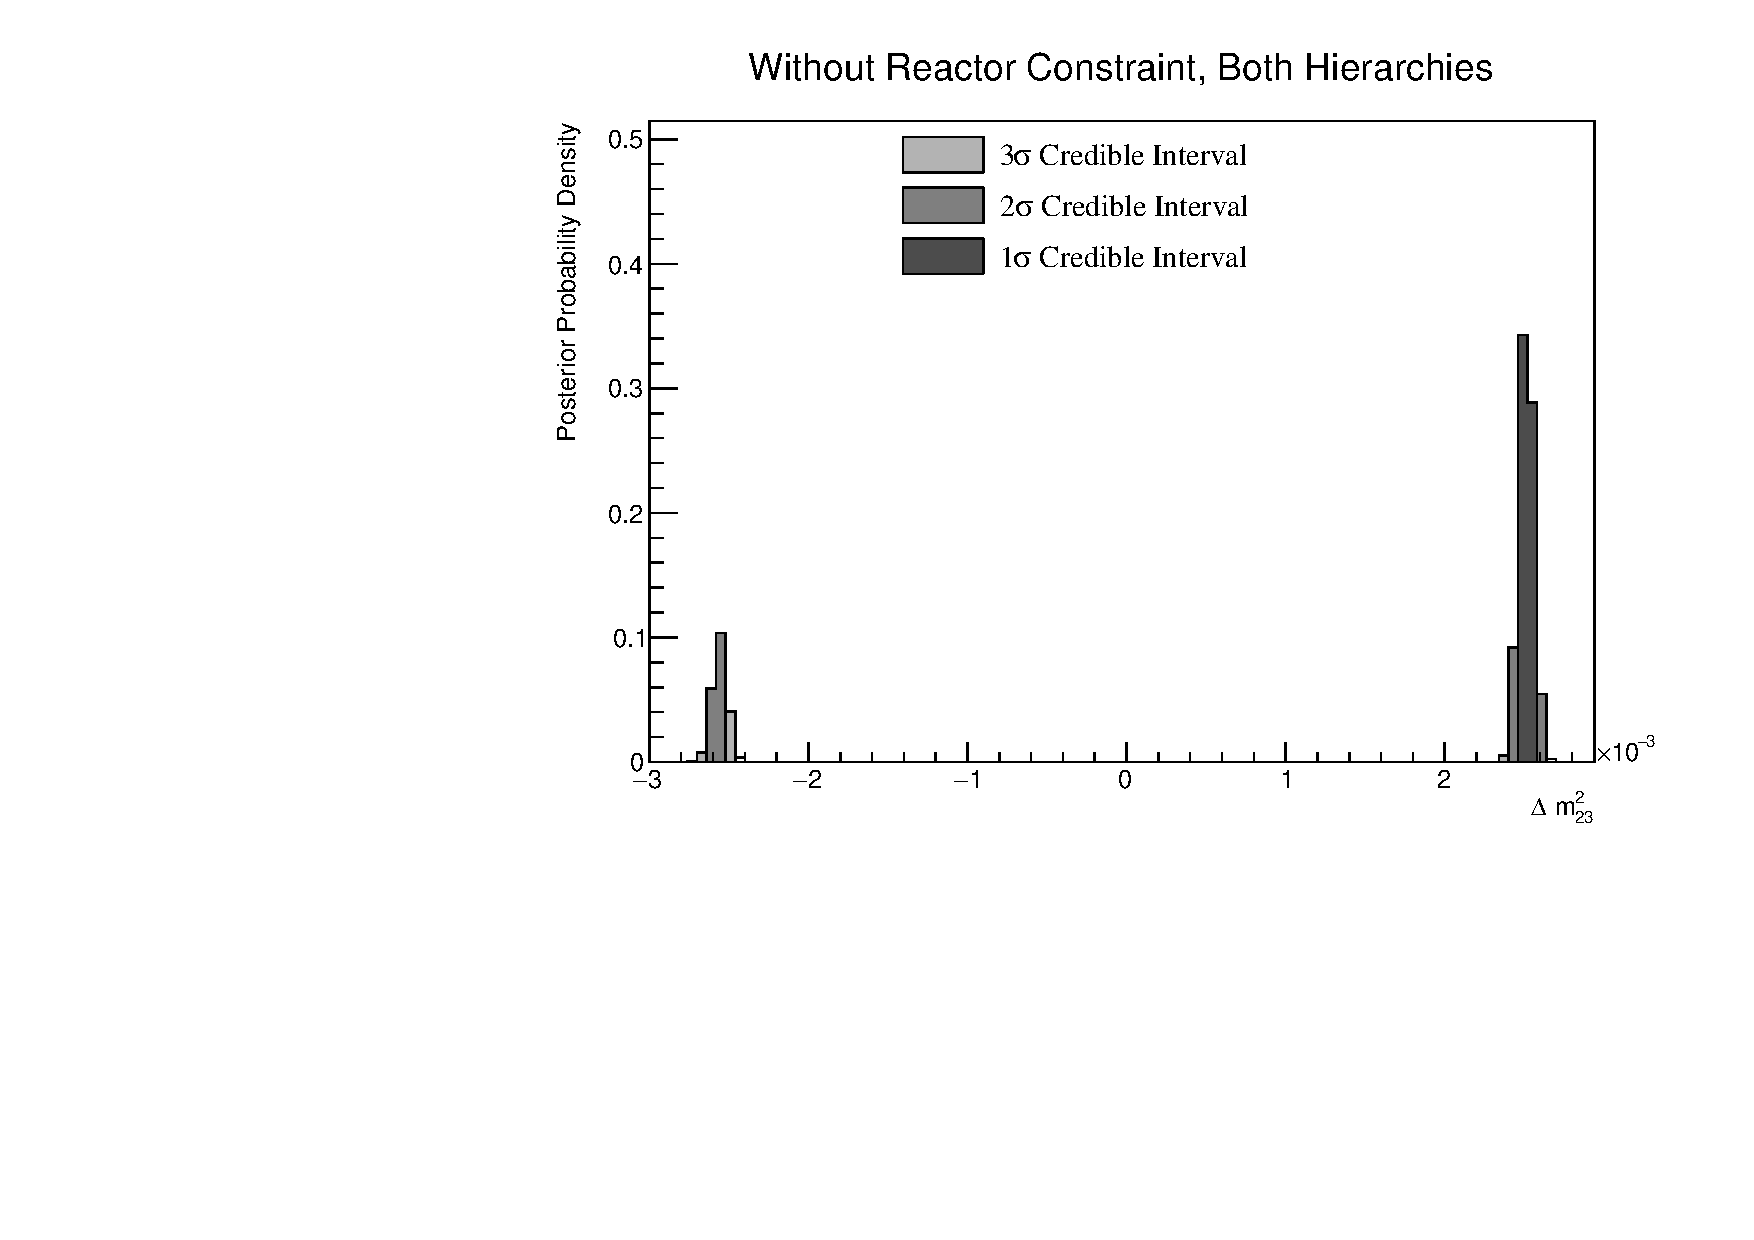
\includegraphics[width=\textwidth, trim={0mm 0mm 0mm 0mm}, clip,page=1]{Figures/OA/JointFit/Contours_1D_dm32_BH_1_woRC_UnSmeared_CredibleInterval.pdf}
  \end{subfigure}
  \caption{The one-dimensional posterior probability density distribution in \quickmath{\Delta m^{2}_{32}}, marginalised over both hierarchies, from the joint beam-atmospheric fit. The reactor constraint is not applied. The vertical dashed line represents the known value of \quickmath{\Delta m^{2}_{32}}.}
  \label{fig:OscillationAnalysis_JointFit_DELM32}
\end{figure}

The sensitivity to \quickmath{\sin^{2}(\theta_{23})} is presented in \autoref{fig:OscillationAnalysis_JointFit_TH23}. There is a clear preference for the upper octant but the peak of the distribution is relatively flat. It peaks at \quickmath{\sin^{2}(\theta_{23}) = 0.509 \pm 0.003} which is in the region of the known value of \quickmath{\sin^{2}(\theta_{23}) = 0.528}. The difference in the highest posterior distribution and the width of the credible interval is relatively unchanged when considering different hierarchy hypotheses showing no strong correlation between \quickmath{\sin^{2}(\theta_{23})} and \quickmath{|\Delta m^{2}_{32}|}.

\begin{figure}[h]
  \begin{subfigure}[t]{0.98\textwidth}
    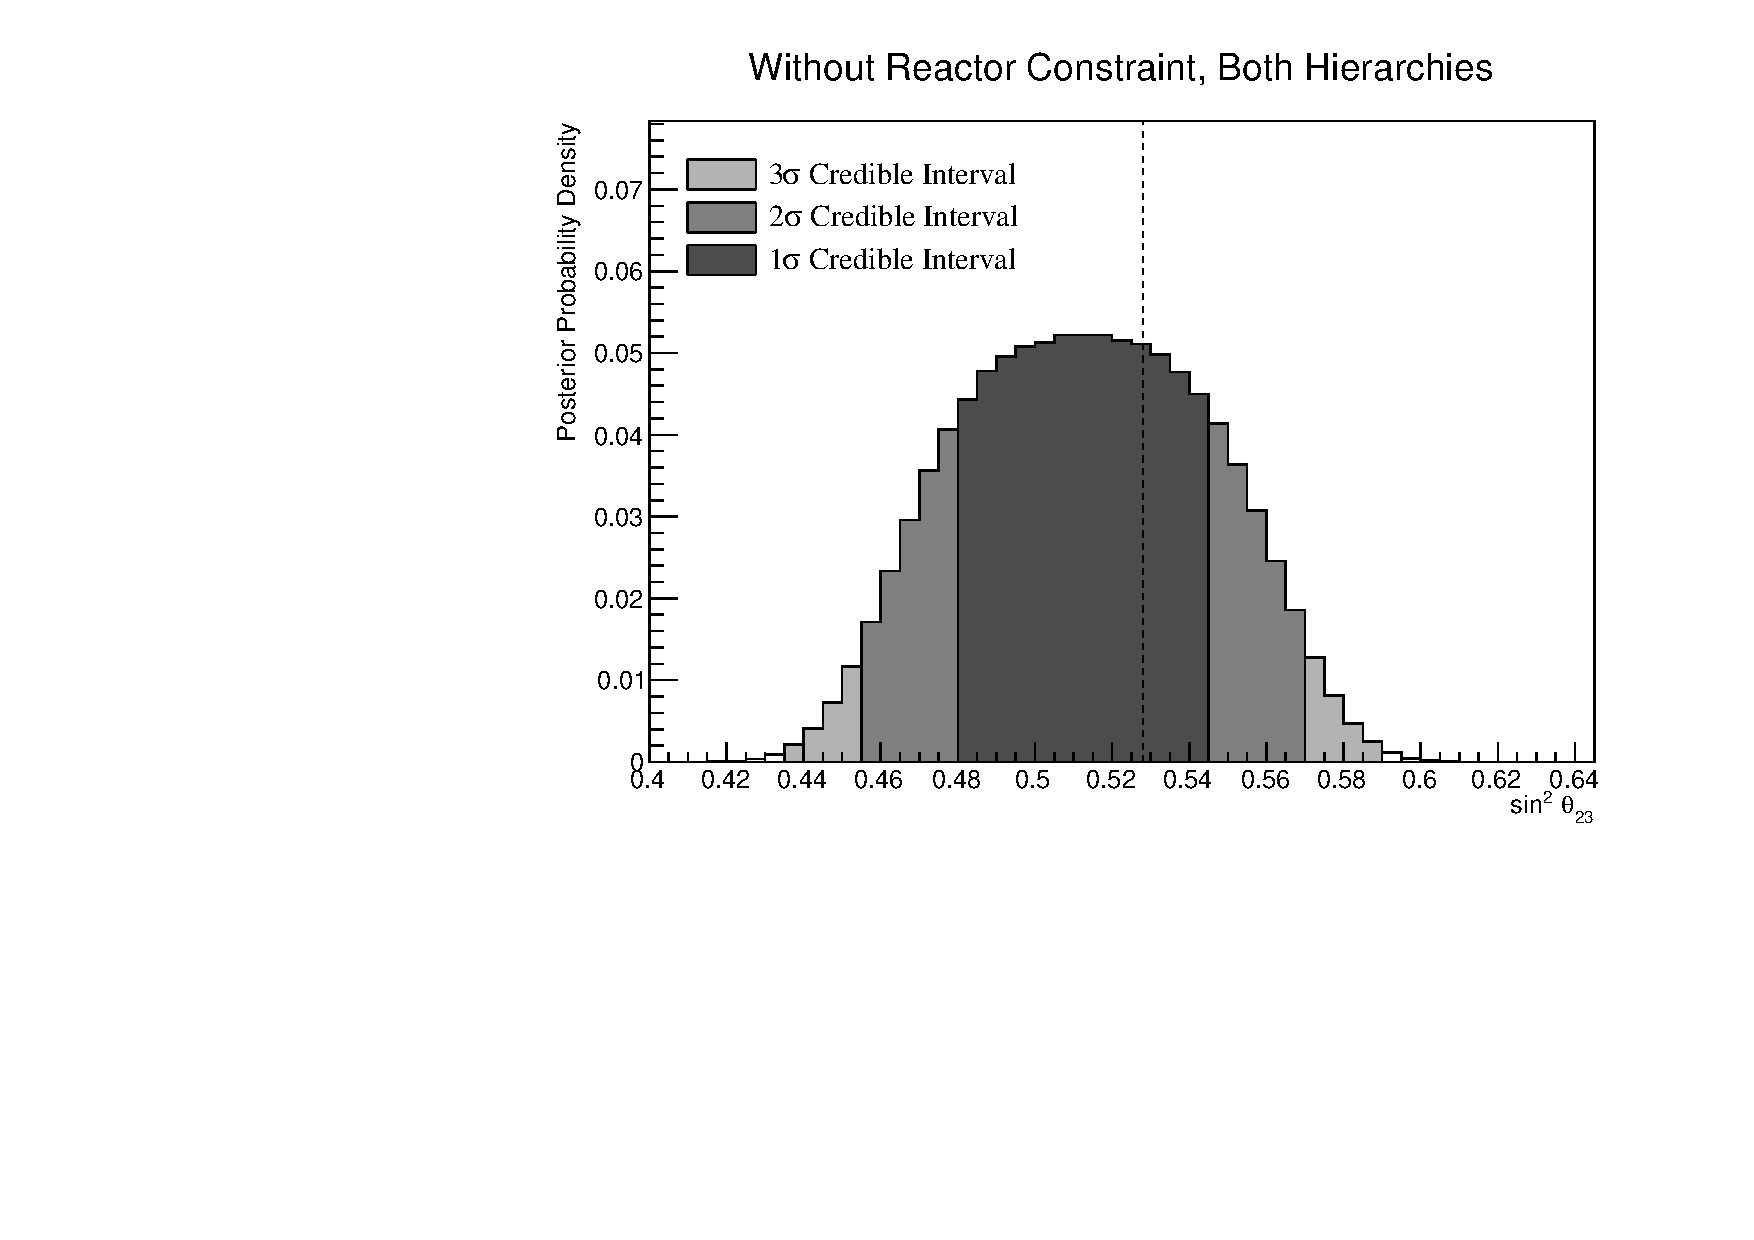
\includegraphics[width=\textwidth, trim={0mm 0mm 0mm 0mm}, clip,page=1]{Figures/OA/JointFit/Contours_1D_th23_BH_1_woRC_UnSmeared_CredibleInterval.pdf}
  \end{subfigure}
  \caption{The one-dimensional posterior probability density distribution in \quickmath{\sin^{2}(\theta_{23})}, marginalised over both hierarchies, from the joint beam-atmospheric fit. The reactor constraint is not applied. The vertical dashed line represents the known value of \quickmath{\sin^{2}(\theta_{23})}.}
  \label{fig:OscillationAnalysis_JointFit_TH23}
\end{figure}

The sensitivity presented as a function of the appearance parameters (\quickmath{\sin^{2}(\theta_{13})\text{\textendash}\delta_{CP}}) is given in \autoref{fig:OscillationAnalysis_JointFit_DCPTH13}. As expected, the contours follow the likelihood shape given in \autoref{fig:OscillationAnalysis_2DLLHOscScans_App}, where the \quickmath{2\sigma} credible intervals have a closed contour excluding the region around \quickmath{\delta_{CP} \sim 1.2}. The width of the \quickmath{3\sigma} credible interval in \quickmath{\sin^{2}(\theta_{13})} is dependent upon the value of \quickmath{\delta_{CP}}. Close to the Asimov point, \quickmath{\delta_{CP} = -1.601}, the width of the \quickmath{3\sigma} credible interval approximately spans \quickmath{\sin^{2}(\theta_{13}) = [0.013, 0.04]}. This is reduced to a region of \quickmath{\sin^{2}(\theta_{13}) = [0.023, 0.042]} at the most disfavoured value of \quickmath{\delta_{CP}}.
%This follows the behaviour shown in the likelihood scans.
The \quickmath{1\sigma} credible interval is consistent with the known oscillation parameter. Application of the reactor constraint would be expected to decrease the width of the \quickmath{1\sigma} credible intervals in \quickmath{\delta_{CP}} due to the triangular shape of the posterior probability. 

The sensitivity in terms of the disappearance parameters, \quickmath{\sin^{2}(\theta_{23})\text{\textendash}\Delta m^{2}_{32}}, is given in \autoref{fig:OscillationAnalysis_JointFit_DM32TH23}. The area contained within the IH contours is significantly smaller than the area within the NH contours. The IH credible intervals are also notably tighter in the \quickmath{\sin^{2}(\theta_{23})} dimension. No significant correlation is observed between \quickmath{\sin^{2}(\theta_{23})} and \quickmath{|\Delta m^{2}_{32}|}.
%In this two-dimensional projection of the posterior distribution, a small section of the \quickmath{1\sigma} credible interval is contained within the inverse hierarchy region. That IH region is clearly favouring the upper octant as expected. The \quickmath{1\sigma} credible region of the NH contour spans both octants but favours the UO.

\begin{figure}[h]
  \begin{subfigure}[t]{0.95\textwidth}
    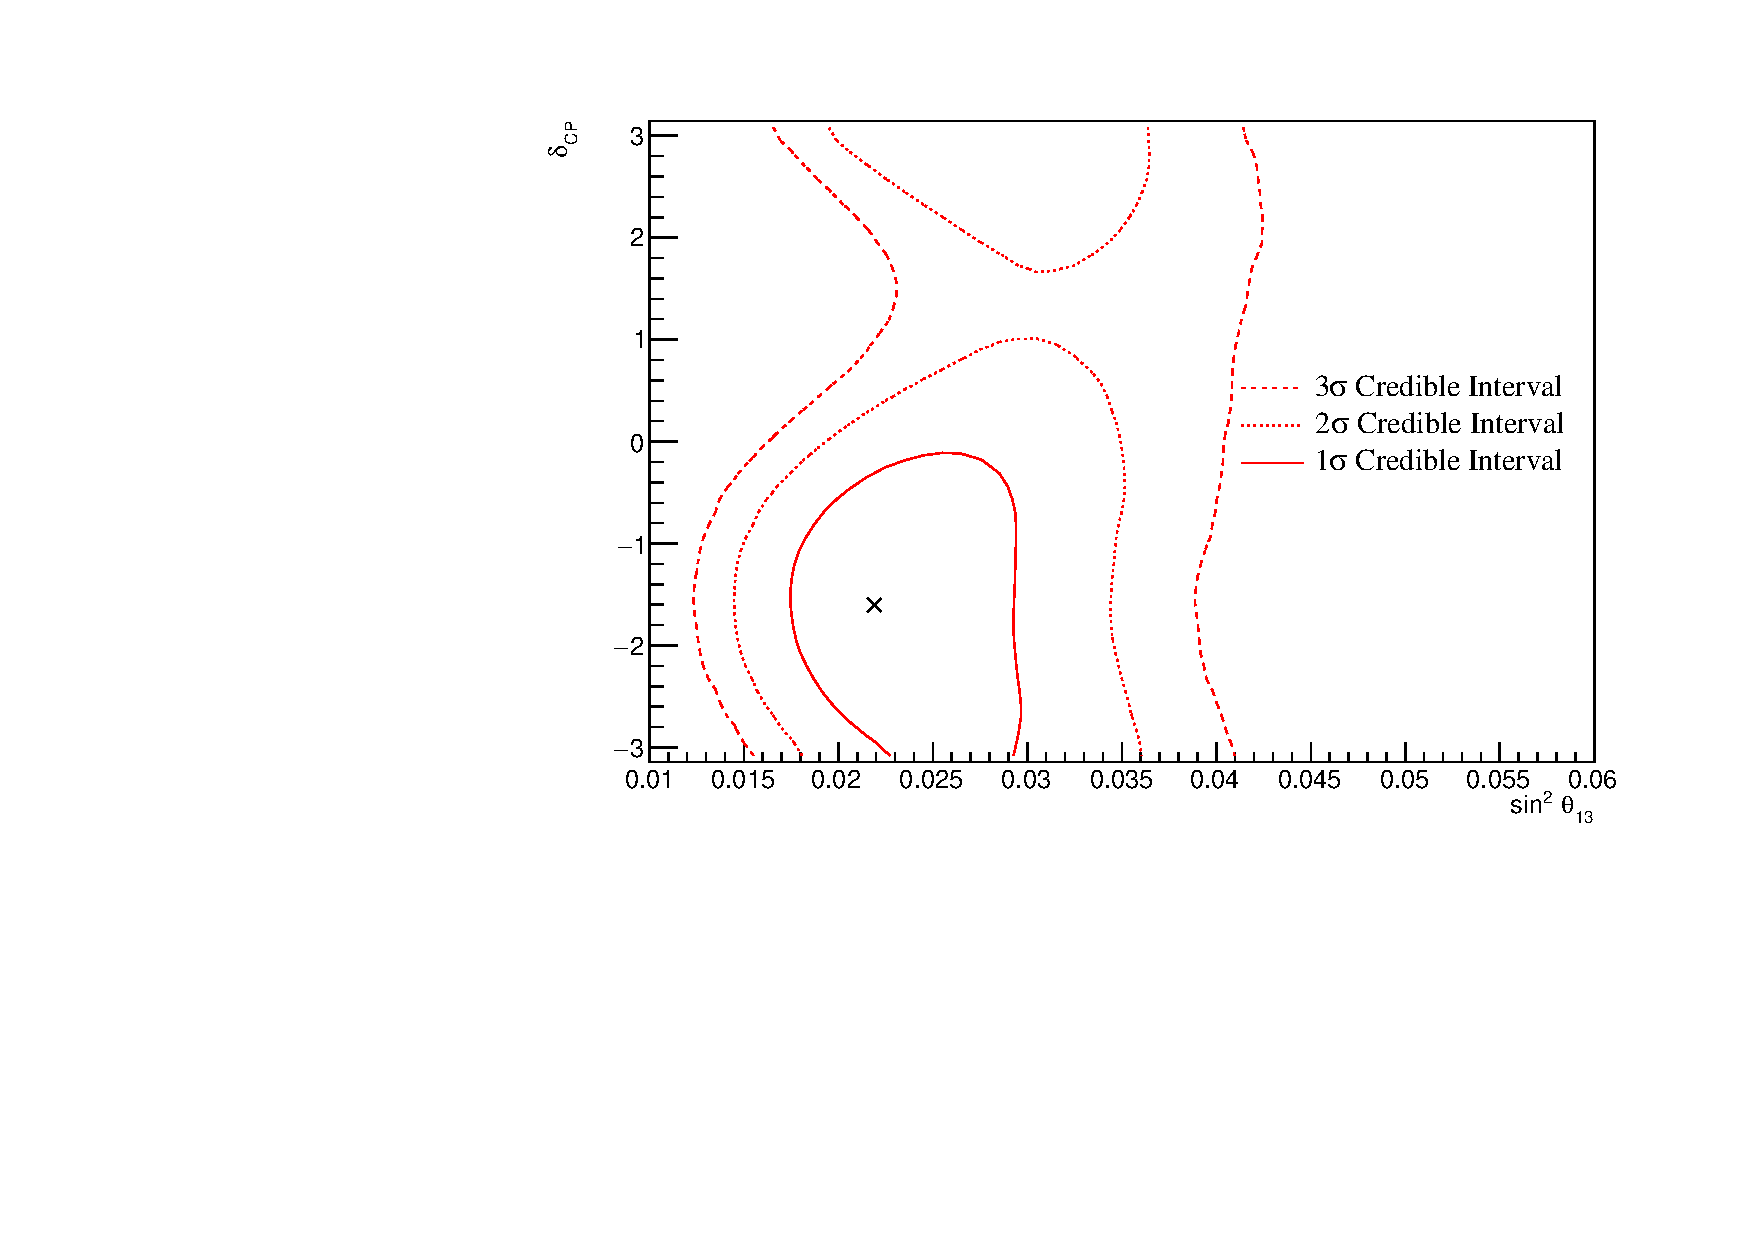
\includegraphics[width=\textwidth, trim={0mm 0mm 0mm 0mm}, clip,page=1]{Figures/OA/JointFit/Contours_2D_th13_dcp_BH_1_woRC_UnSmeared_CredibleInterval.pdf}
  \end{subfigure}
  \caption{The two-dimensional posterior probability density distribution in \quickmath{\delta_{CP}\text{\textendash}\sin^{2}(\theta_{13})}, marginalised over both hierarchies, from the joint beam-atmospheric fit. The reactor constraint is not applied. The marker represents the known value of \quickmath{\delta_{CP}\text{\textendash}\sin^{2}(\theta_{13})}.}
  \label{fig:OscillationAnalysis_JointFit_DCPTH13}
\end{figure}

\begin{figure}[h]
  \begin{subfigure}[t]{0.95\textwidth}
    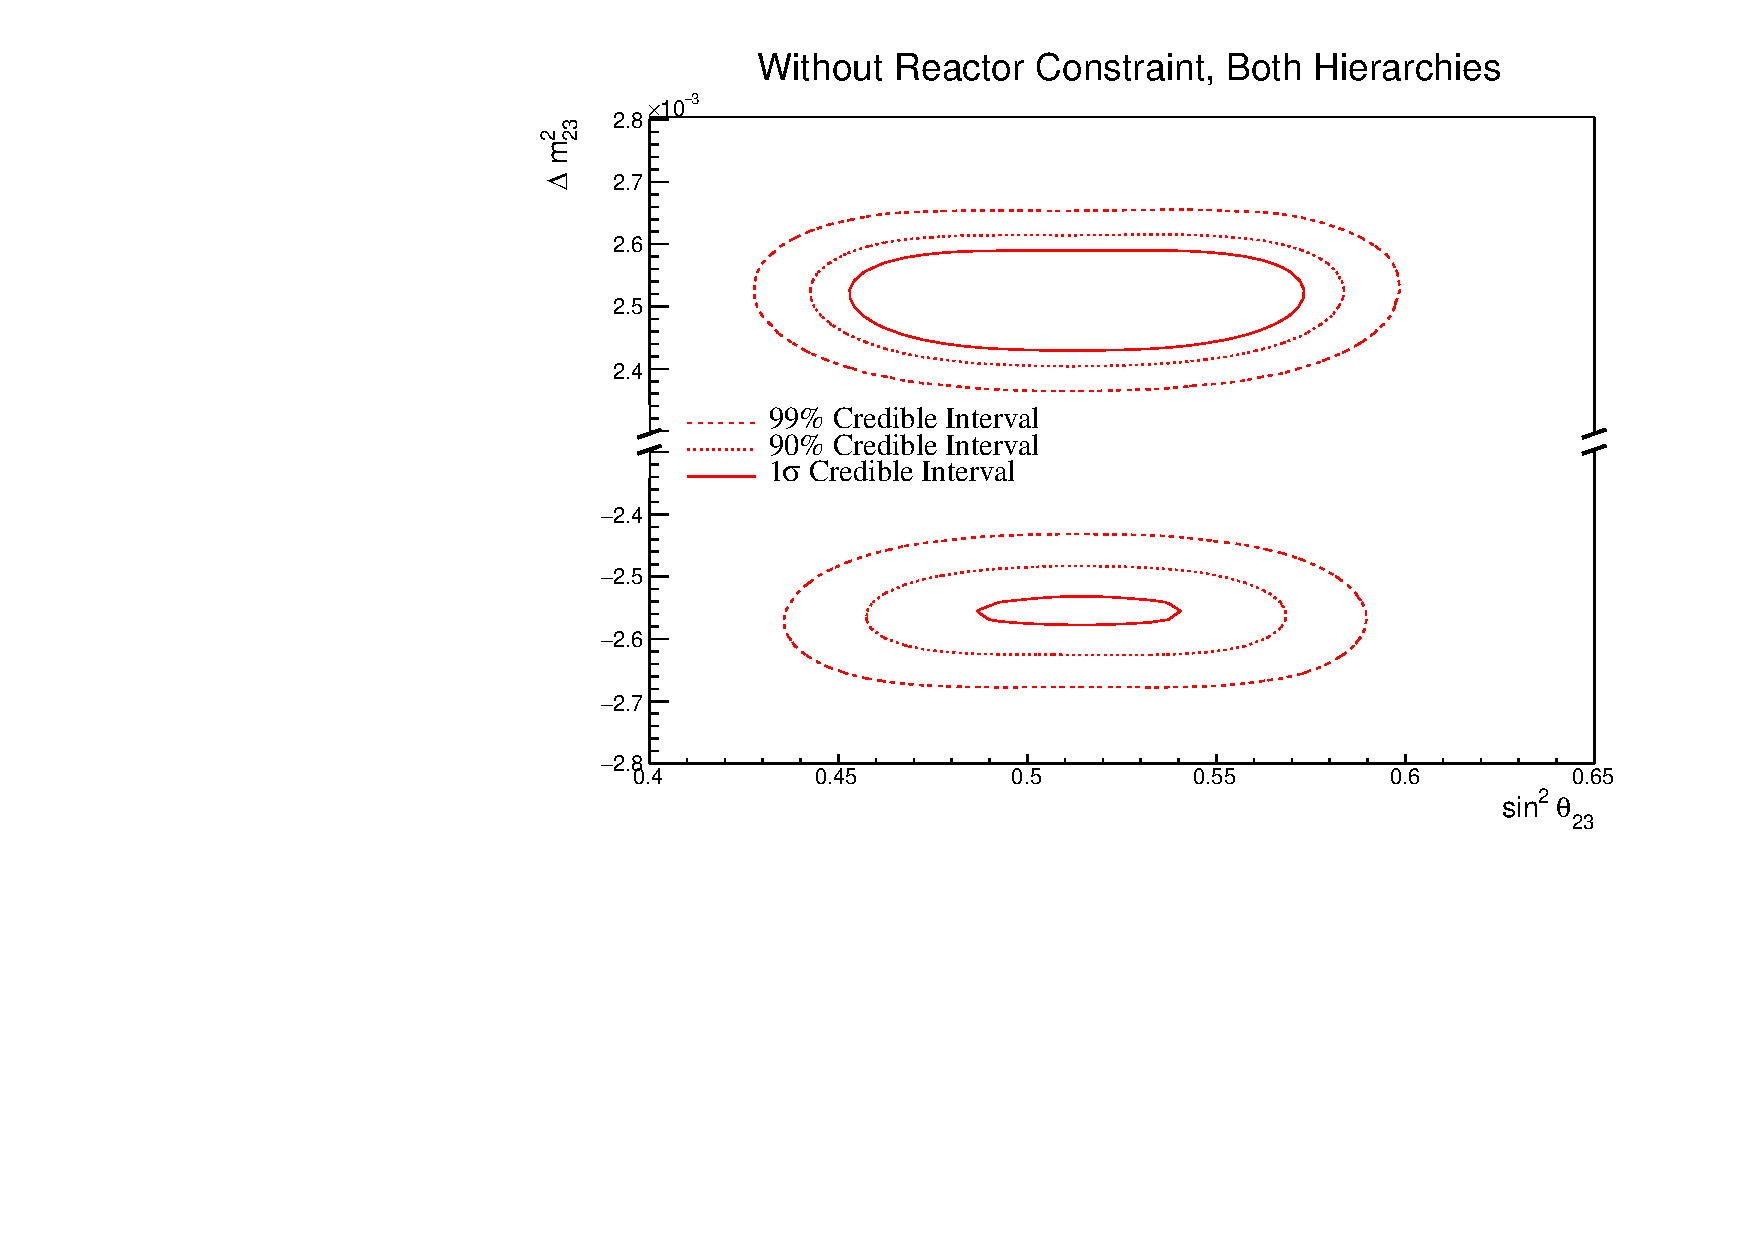
\includegraphics[width=\textwidth, trim={0mm 0mm 0mm 0mm}, clip,page=1]{Figures/OA/JointFit/Contours_2D_th23_dm32_BH_0_woRC_UnSmeared_CredibleInterval.pdf}
  \end{subfigure}
  \caption{The two-dimensional posterior probability density distribution in \quickmath{\Delta m^{2}_{32}\text{\textendash}\sin^{2}(\theta_{23})}, marginalised over both hierarchies, from the joint beam-atmospheric fit. The reactor constraint is not applied. The marker represents the known value of \quickmath{\Delta m^{2}_{32}\text{\textendash}\sin^{2}(\theta_{23})}.}
  \label{fig:OscillationAnalysis_JointFit_DM32TH23}
\end{figure}


The two-dimensional posterior distribution for each permutation of the oscillation parameters of interest is given in \autoref{fig:OscillationAnalysis_JointFit_TriPlot}. The most notable observation is that the \quickmath{\sin^{2}(\theta_{13})} and \quickmath{\sin^{2}(\theta_{23})} are anti-correlated. If the value of \quickmath{\sin^{2}(\theta_{13})} was constrained closer to the known oscillation parameter value, the preferred value of \quickmath{\sin^{2}(\theta_{23})} would increase. This would move the highest posterior probability closer in line with the known value and could lead to an increase in the preference for the correct octant hypothesis (UO).

Furthermore, the \quickmath{\delta_{CP}} and \quickmath{|\Delta m^{2}_{32}|} oscillation parameters are anti-correlated, such that higher values of \quickmath{|\Delta m^{2}_{32}|} prefer lower values of \quickmath{\delta_{CP}}. Whilst this is an interesting result on its own, the width of the \quickmath{\Delta m^{2}_{32}} contours also depend on \quickmath{\sin^{2}(\theta_{13})}. This introduces another correlation effect that could modify the sensitivity to \quickmath{\delta_{CP}} once the reactor constraint is applied.

\begin{figure}[h]
  \begin{subfigure}[t]{0.98\textwidth}
    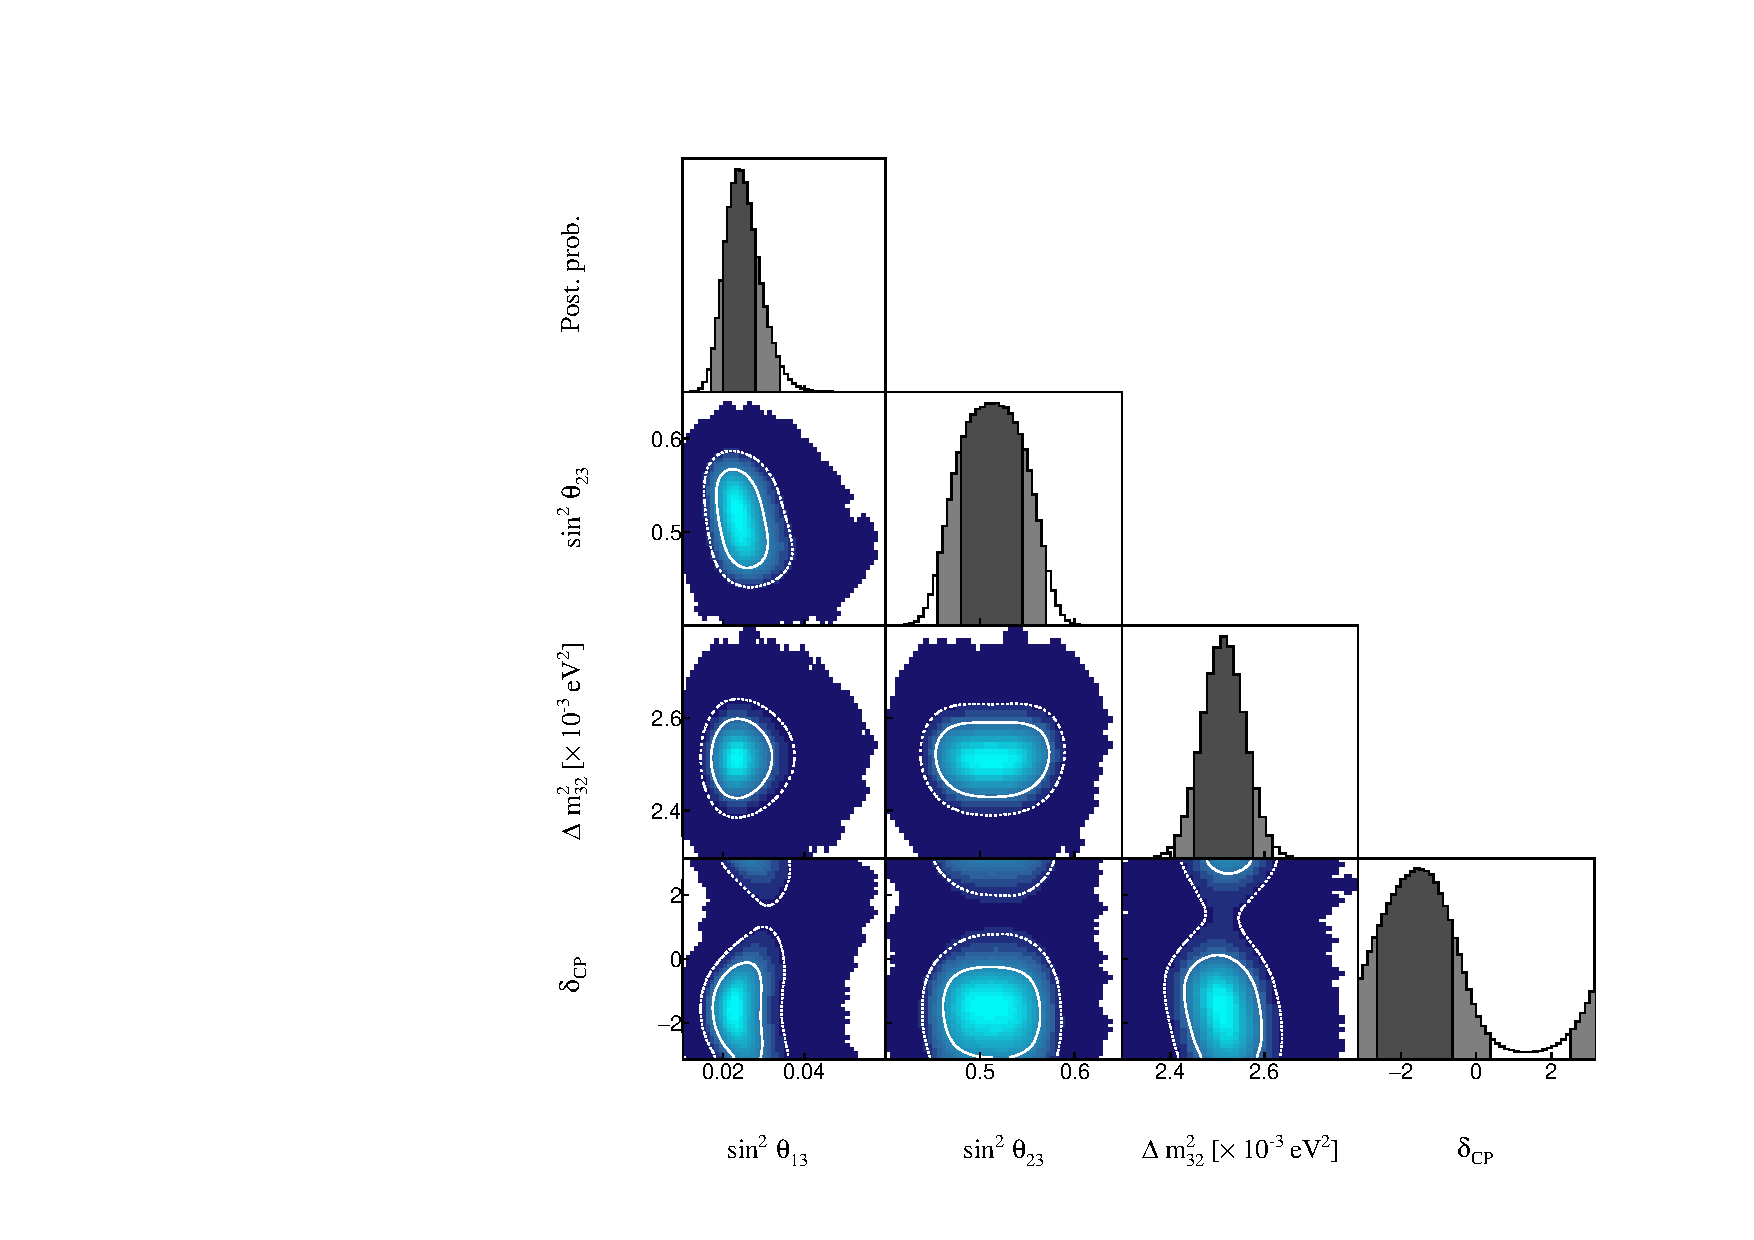
\includegraphics[width=\textwidth, trim={0mm 0mm 0mm 0mm}, clip,page=1]{Figures/OA/JointFit/Contours_1D_woRC_UnSmeared_CredibleInterval_TrianglePlot.pdf}
  \end{subfigure}
  \caption{The posterior probability density distribution from the joint beam-atmospheric fit. The reactor constraint is not applied. The distribution is given for each two-dimensional permutation of the oscillation parameters of interest. The one-dimensional distribution of each parameter is also given.}
  \label{fig:OscillationAnalysis_JointFit_TriPlot}
\end{figure}

The correlation between \quickmath{\sin^{2}(\theta_{13})} and \quickmath{\Delta m^{2}_{32}} can be seen in \autoref{fig:OscillationAnalysis_JointFit_DM32TH13}. A much larger fraction of the posterior distribution is contained in the NH for lower values of \quickmath{\sin^{2}(\theta_{13})}. Consequently, the application of the reactor constraint would be expected to significantly increase the preference for NH.

\begin{figure}[h]
  \begin{subfigure}[t]{0.98\textwidth}
    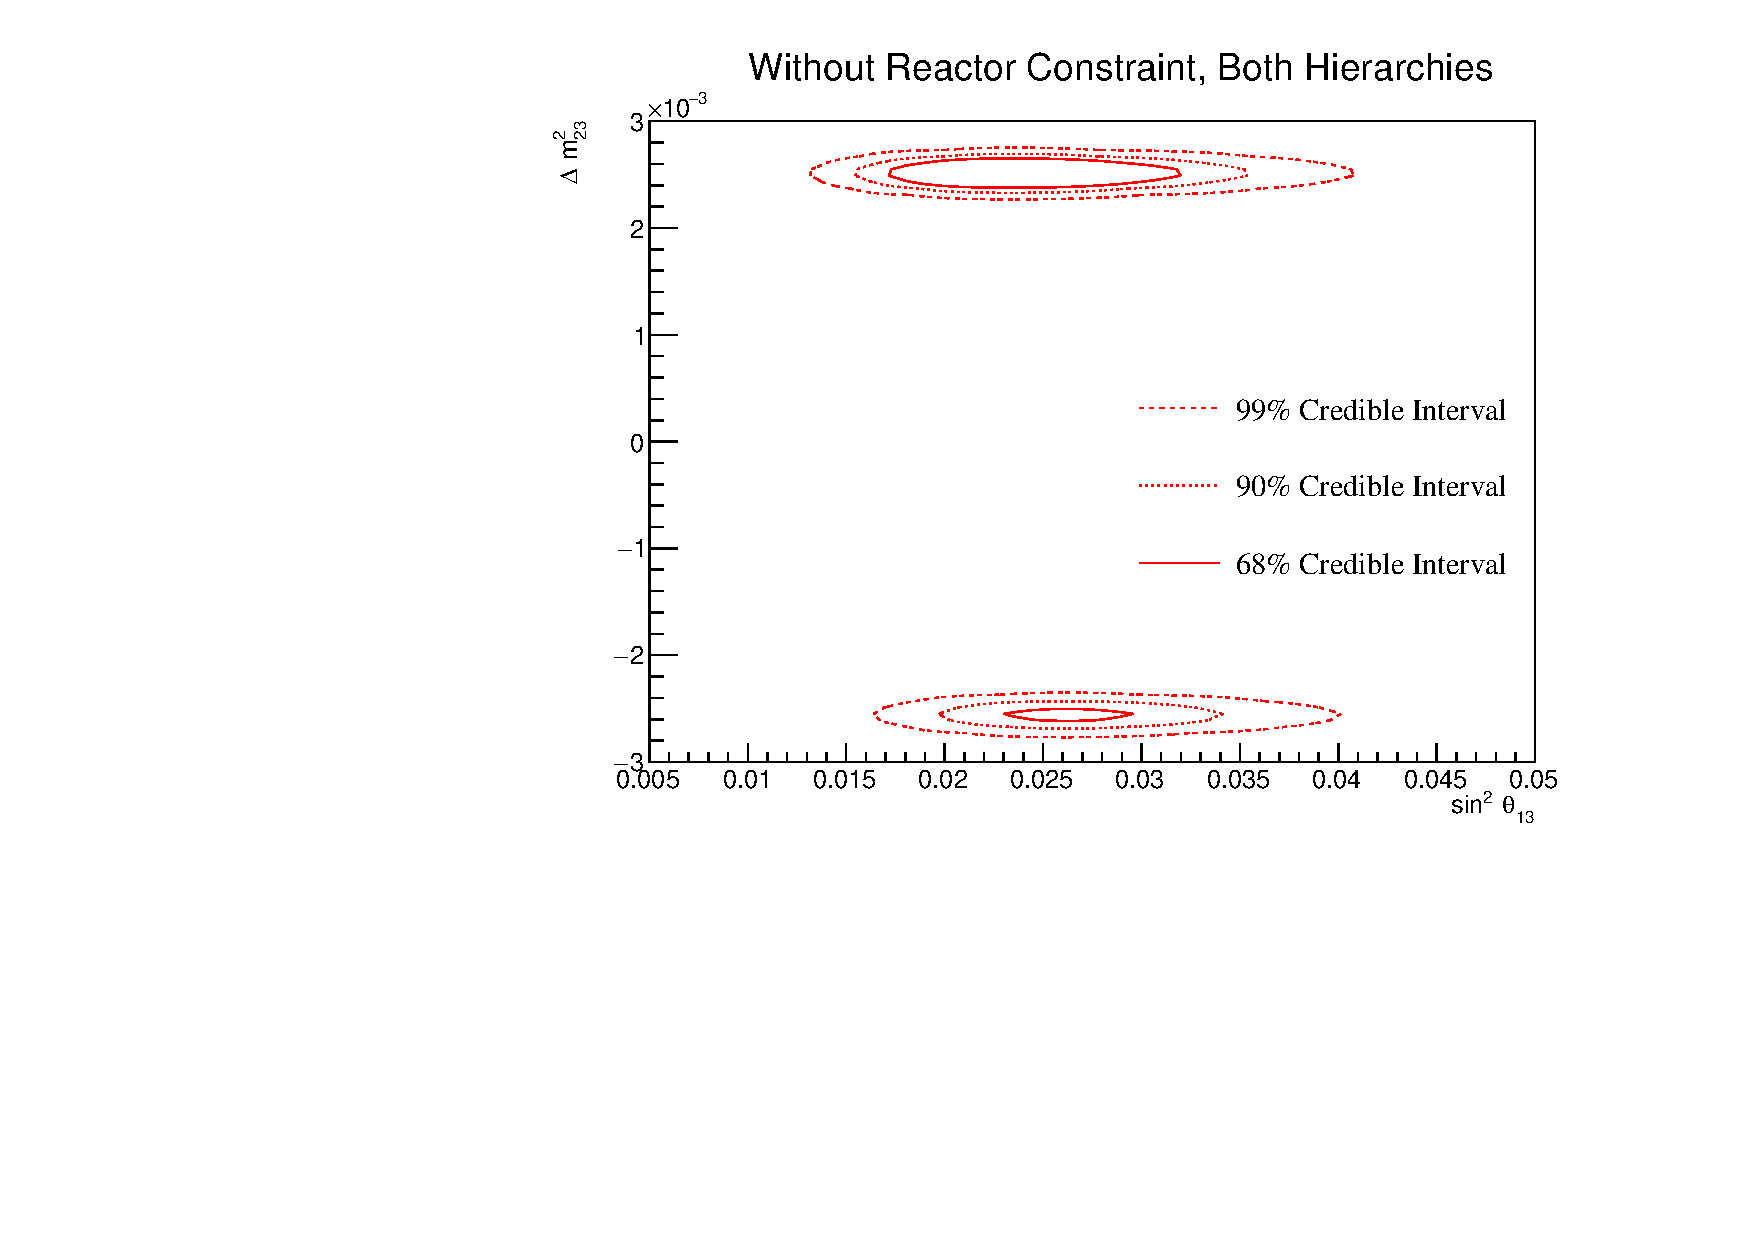
\includegraphics[width=\textwidth, trim={0mm 0mm 0mm 0mm}, clip,page=1]{Figures/OA/JointFit/Contours_2D_th13_dm32_BH_0_woRC_UnSmeared_CredibleInterval.pdf}
  \end{subfigure}
  \caption{The two-dimensional posterior probability density distribution in \quickmath{\Delta m^{2}_{32}\text{\textendash}\sin^{2}(\theta_{13})}, marginalised over both hierarchies, from the joint beam-atmospheric fit. The reactor constraint is not applied. The marker represents the known value of \quickmath{\Delta m^{2}_{32}\text{\textendash}\sin^{2}(\theta_{13})}.}
  \label{fig:OscillationAnalysis_JointFit_DM32TH13}
\end{figure}

\clearpage
\subsection{Atmospheric and Beam Sensitivity with Reactor Constraint}
\label{sec:OscillationAnalysis_JointFit_wRC}

This section presents the sensitivities of the joint beam-atmospheric fit when the reactor constraint is applied to \quickmath{\sin^{2}(\theta_{13})}. As with the previous studies, the Asimov data is made using the AsimovA oscillation parameter set defined in \autoref{tab:Theory_ParameterSets} and the post-BANFF systematic parameter tune.
  
\begin{figure}[h]
  \begin{subfigure}[t]{0.98\textwidth}
    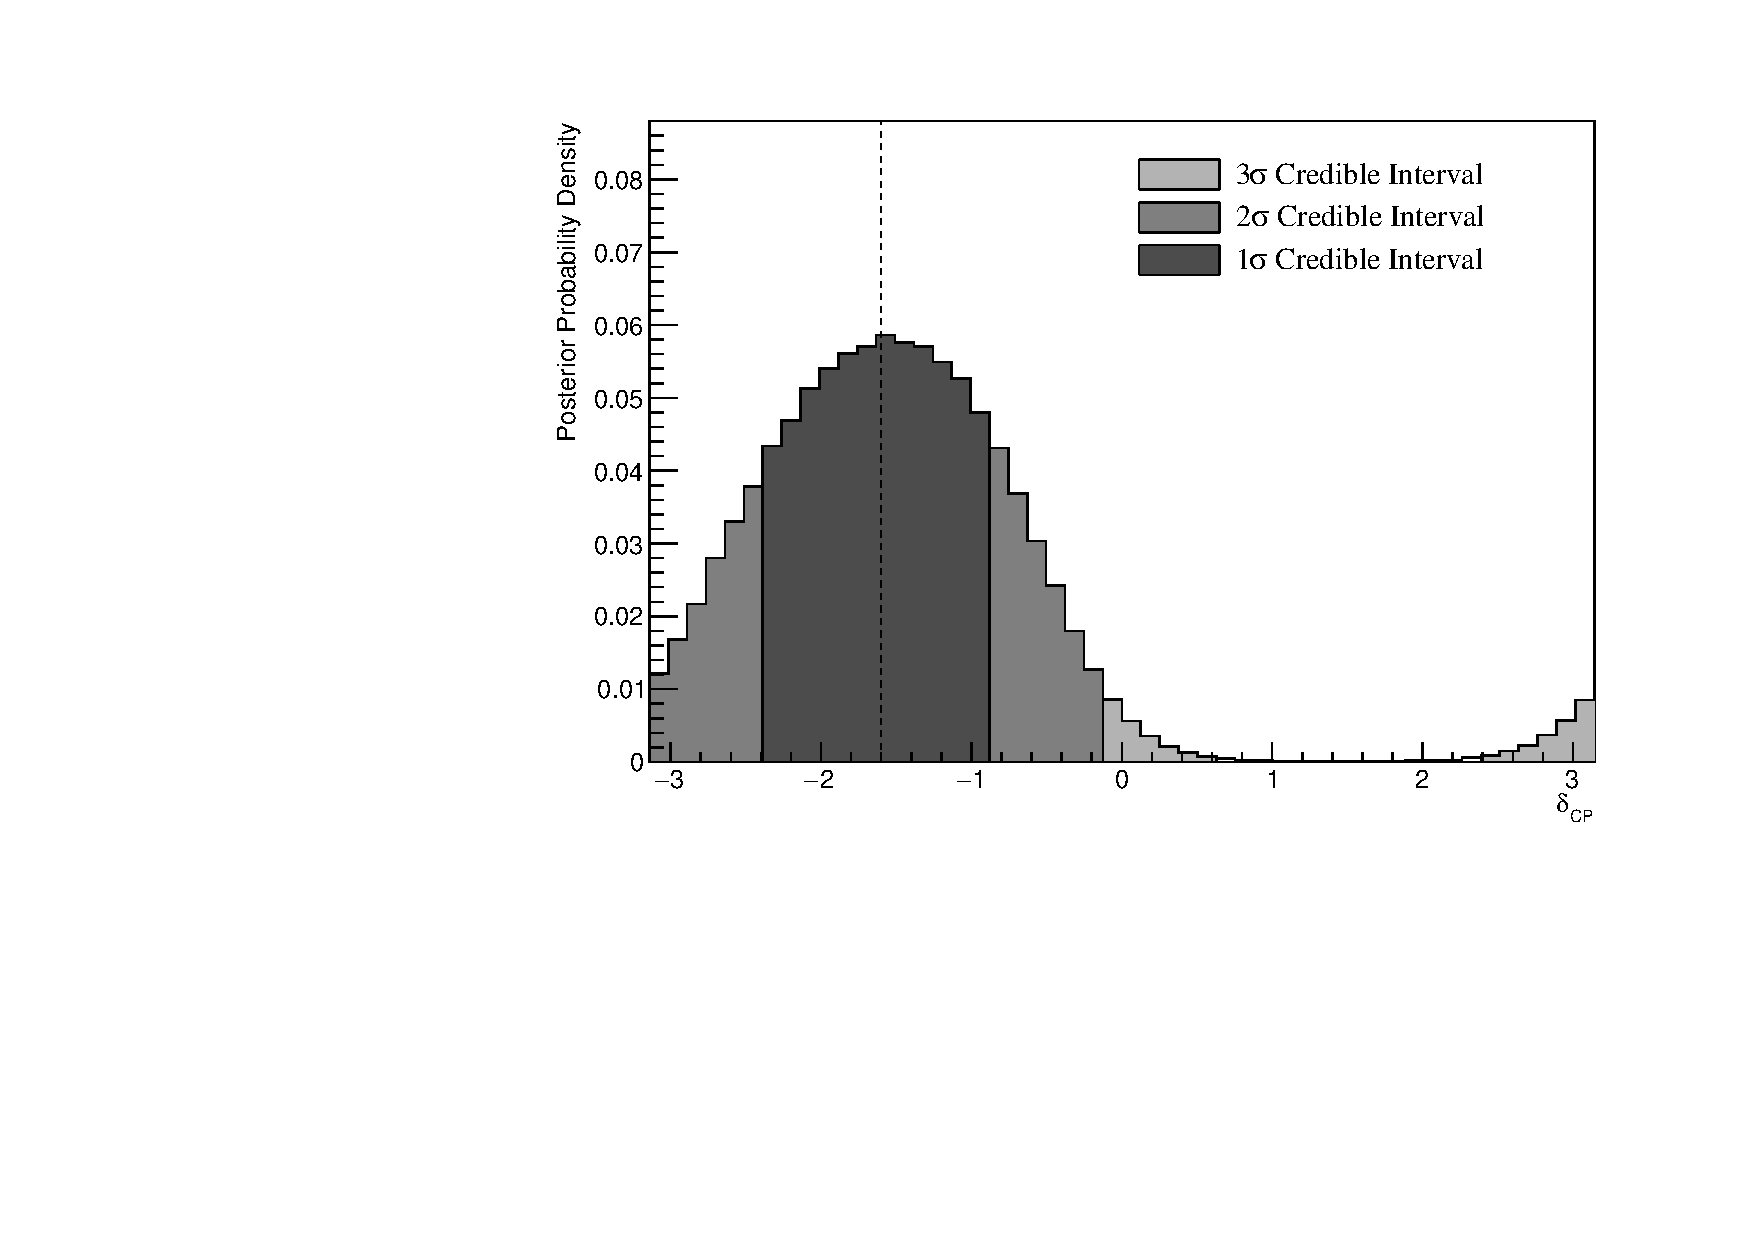
\includegraphics[width=\textwidth, trim={0mm 0mm 0mm 0mm}, clip,page=1]{Figures/OA/JointFit_wRC/Contours_1D_dcp_BH_1_wRC_UnSmeared_CredibleInterval.pdf}
  \end{subfigure}
  \caption{The one-dimensional posterior probability density distribution in \quickmath{\delta_{CP}}, marginalised over both hierarchies, from the joint beam-atmospheric fit where the reactor constraint is applied. The vertical dashed line represents the known value of \quickmath{\delta_{CP}}.}
  \label{fig:OscillationAnalysis_JointFit_wRC_DCP}
\end{figure}

\autoref{fig:OscillationAnalysis_JointFit_wRC_DCP} illustrates the sensitivity to \quickmath{\delta_{CP}}, marginalised over both hierarchies. The CP-conserving value of \quickmath{\delta_{CP} = 0} is disfavoured at \quickmath{2\sigma} whilst the value of \quickmath{\delta_{CP} = \pm\pi} is very close to being disfavoured at \quickmath{2\sigma}. Furthermore, the \quickmath{3\sigma} credible interval excludes the region of \quickmath{\delta_{CP} = [0.63,2.39]}, thus clearly disfavouring the region of \quickmath{\delta_{CP} = \pi/2} at more than \quickmath{3\sigma} for this particular set of known oscillation parameters. The width of the \quickmath{1\sigma} credible intervals and the position of the highest posterior probability density is given in \autoref{tab:OscillationAnalysis_JointFit_wRC_CredIntervals}. The highest posterior probability density in \quickmath{\delta_{CP}} is calculated as \quickmath{\delta_{CP} = -1.57 \pm 0.07} showing no significant biases in the determination of the known oscillation parameters.
%The posterior distribution is more peaked around the known oscillation parameter value of \quickmath{\delta_{CP} = -1.601}, as compared to the sensitivities when the reactor constraint is not applied (\autoref{sec:OscillationAnalysis_JointFit}). 

The effect of applying the reactor constraint for \quickmath{\delta_{CP}} in the joint beam-atmospheric fit is presented in \autoref{fig:OscillationAnalysis_JointFit_wRC_Comp_DCP}. The reactor constraint significantly improves the ability of the fit to select the known parameter value. This behaviour is evidenced by the tightening of the \quickmath{1\sigma} and \quickmath{90\%} credible intervals and the disfavoured region, centered at \quickmath{\delta_{CP} \sim \pi/2}, becoming wider when the reactor constraint is applied. This follows from the correlations shown in \autoref{fig:OscillationAnalysis_JointFit_DCPTH13}, where a lower value of \quickmath{\sin^{2}(\theta_{13})} results in tighter constraints on \quickmath{\delta_{CP}}. 

\begin{figure}[h]
  \begin{subfigure}[t]{0.98\textwidth}
    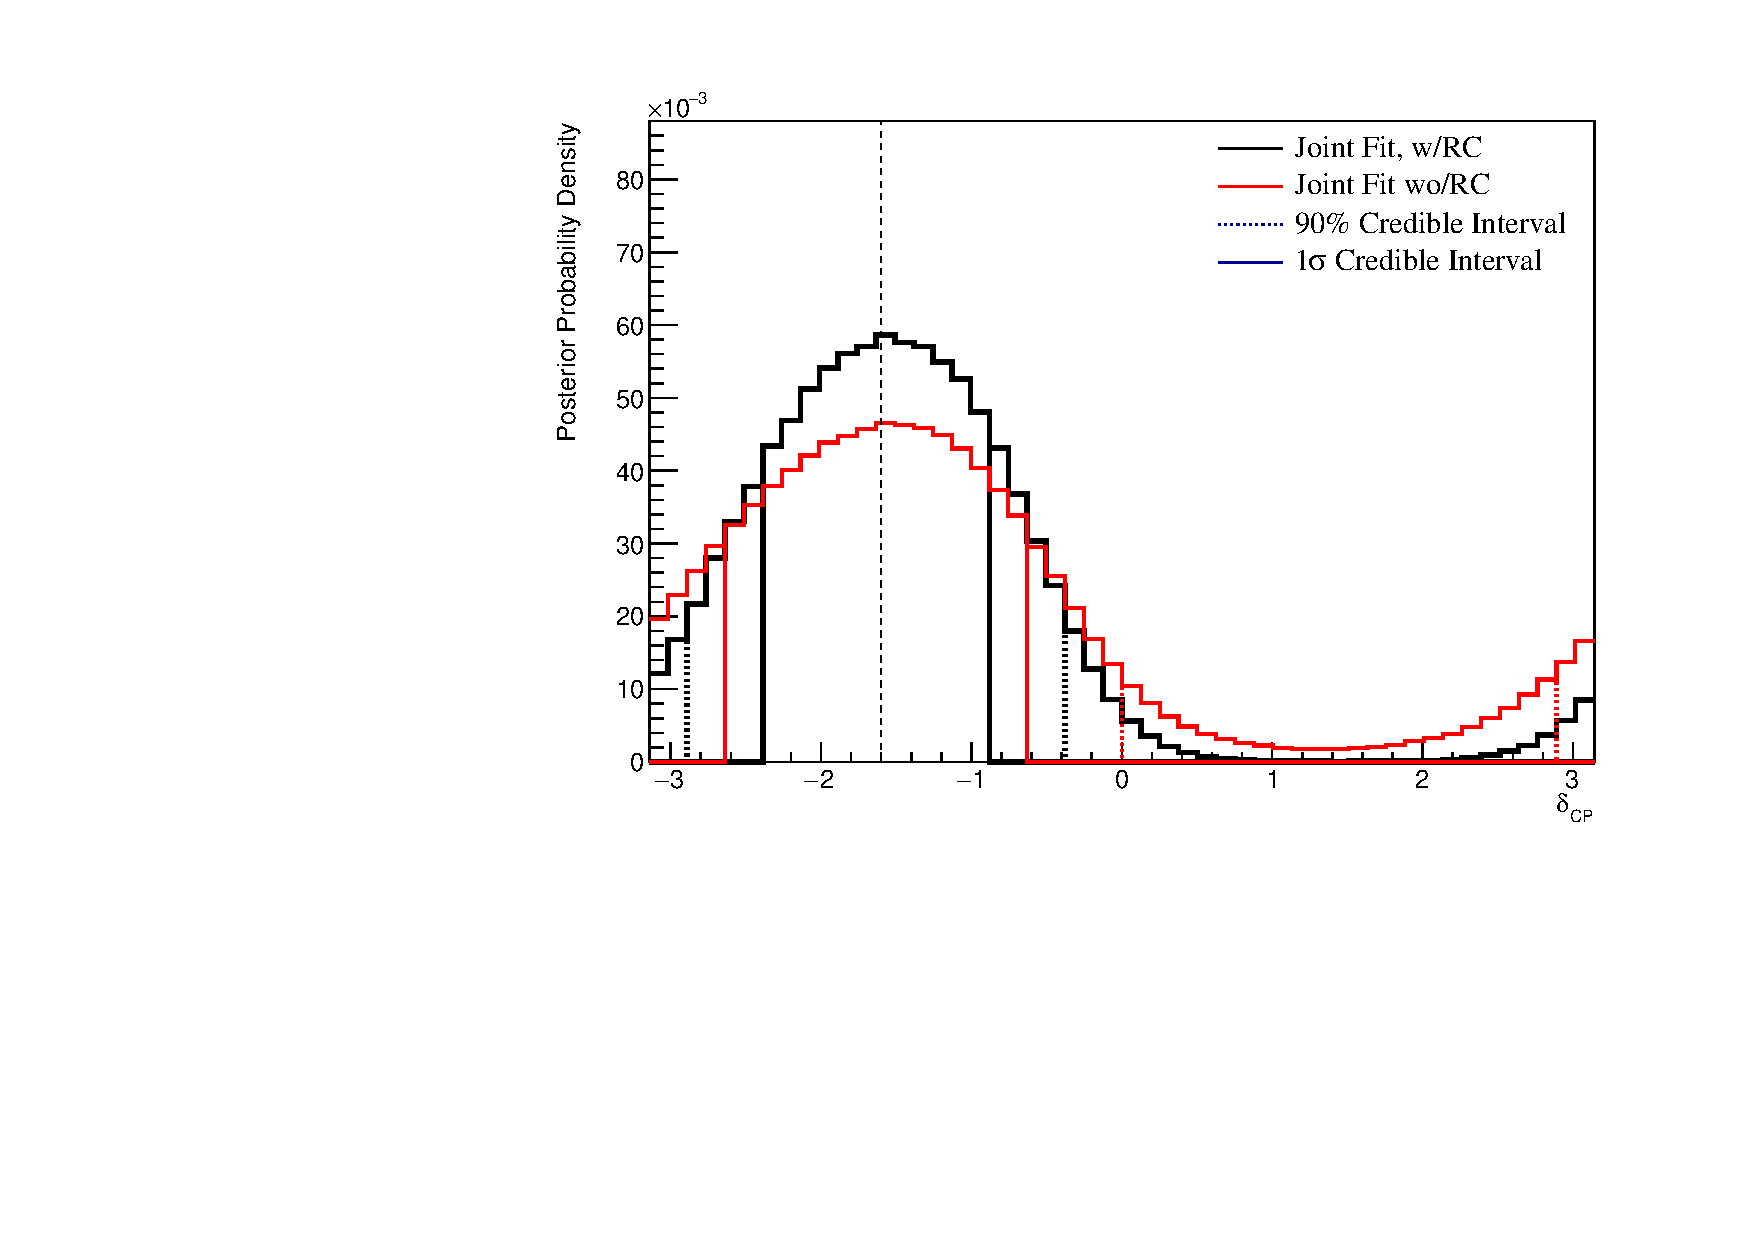
\includegraphics[width=\textwidth, trim={0mm 0mm 0mm 0mm}, clip,page=1]{Figures/OA/JointFit_wRC_Comp/ContourComparison_1D_dcp_BH_2_wRC_woRC_UnSmeared_CredibleInterval.pdf}
  \end{subfigure}
  \caption{The one-dimensional posterior probability density distribution in \quickmath{\delta_{CP}} compared between the joint beam-atmospheric fit (Red) and the joint beam-atmospheric fit with the reactor constraint (Black). The distributions are marginalised over both hierarchies. The vertical dashed line represents the known value of \quickmath{\delta_{CP}}.}
  \label{fig:OscillationAnalysis_JointFit_wRC_Comp_DCP}
\end{figure}

\begin{table}[ht!]
  \centering
  \begingroup
  \renewcommand{\arraystretch}{1.5}
  \begin{tabular}{c|c|c}
    Parameter               & Interval & HPD \\ \hline
    \quickmath{\delta_{CP}, \text{ (BH)}} & \quickmath{\left[ -2.39, -0.88 \right]} & \quickmath{-1.57 \pm 0.07} \\
    \quickmath{\delta_{CP}, \text{ (NH)}} & \quickmath{\left[ -2.39, -0.75 \right]} & \quickmath{-1.57 \pm 0.07} \\
    \quickmath{\delta_{CP}, \text{ (IH)}} & \quickmath{\left[ -2.14, -1.01 \right]} & \quickmath{-1.57 \pm 0.07} \\ \hline
    \quickmath{\Delta m^{2}_{32} \text{ (BH) } [\times 10^{-3} \text{eV}^{2}]} & \quickmath{\left[ 2.45, 2.56 \right]} & \quickmath{2.51 \pm 0.01} \\
    \quickmath{\Delta m^{2}_{32} \text{ (NH) } [\times 10^{-3} \text{eV}^{2}]} & \quickmath{\left[ 2.47, 2.56 \right]} & \quickmath{2.51 \pm 0.01} \\
    \quickmath{\Delta m^{2}_{32} \text{ (IH) } [\times 10^{-3} \text{eV}^{2}]} & \quickmath{\left[ -2.60, -2.51 \right]} & \quickmath{-2.55 \pm 0.01} \\ \hline
    \quickmath{\sin^{2}(\theta_{23}) \text{ (BH) }} & \quickmath{\left[ 0.490, 0.555 \right]} & \quickmath{0.528 \pm 0.03} \\ 
    \quickmath{\sin^{2}(\theta_{23}) \text{ (NH) }} & \quickmath{\left[ 0.490, 0.555 \right]} & \quickmath{0.528 \pm 0.03} \\ 
    \quickmath{\sin^{2}(\theta_{23}) \text{ (IH) }} & \quickmath{\left[ 0.500, 0.560 \right]} & \quickmath{0.538 \pm 0.03} \\ \hline \hline
  \end{tabular}
  \caption{The position of the highest posterior probability density (HPD) and width of the \quickmath{1\sigma} credible interval for the joint beam-atmospheric fit where the reactor constraint is applied. The values are presented by which hierarchy hypothesis is assumed: marginalised over both hierarchies (BH), normal hierarchy only (NH), and inverted hierarchy only (IH).}
  \label{tab:OscillationAnalysis_JointFit_wRC_CredIntervals}
  \endgroup
\end{table}

The sensitivity to \quickmath{\sin^{2}(\theta_{23})}, marginalised over both hierarchies, is given in \autoref{fig:OscillationAnalysis_JointFit_wRC_TH23}. The highest posterior probability density is located at \quickmath{\sin^{2}(\theta_{23}) = 0.528 \pm 0.03} which agrees with the known value of \quickmath{\sin^{2}(\theta_{23}) = 0.528}. The distribution clearly favours the UO with almost the entirety of the \quickmath{1\sigma} credible interval being contained in that region. \autoref{fig:OscillationAnalysis_JointFit_wRC_Comp_TH23} highlights the sensitivity of the joint fit both with and without the reactor constraint. The fit where the reactor constraint is applied selects the known value much better. This is a result of the marginalisation effects between the \quickmath{\sin^{2}(\theta_{13})} and \quickmath{\sin^{2}(\theta_{23})} parameters, as observed in \autoref{fig:OscillationAnalysis_JointFit_TriPlot}.
%The posterior distribution of the fit with reactor constraint is more peaked compared to the flatter distribution when the reactor constraint is not applied. 

\begin{figure}[h]
  \begin{subfigure}[t]{0.98\textwidth}
    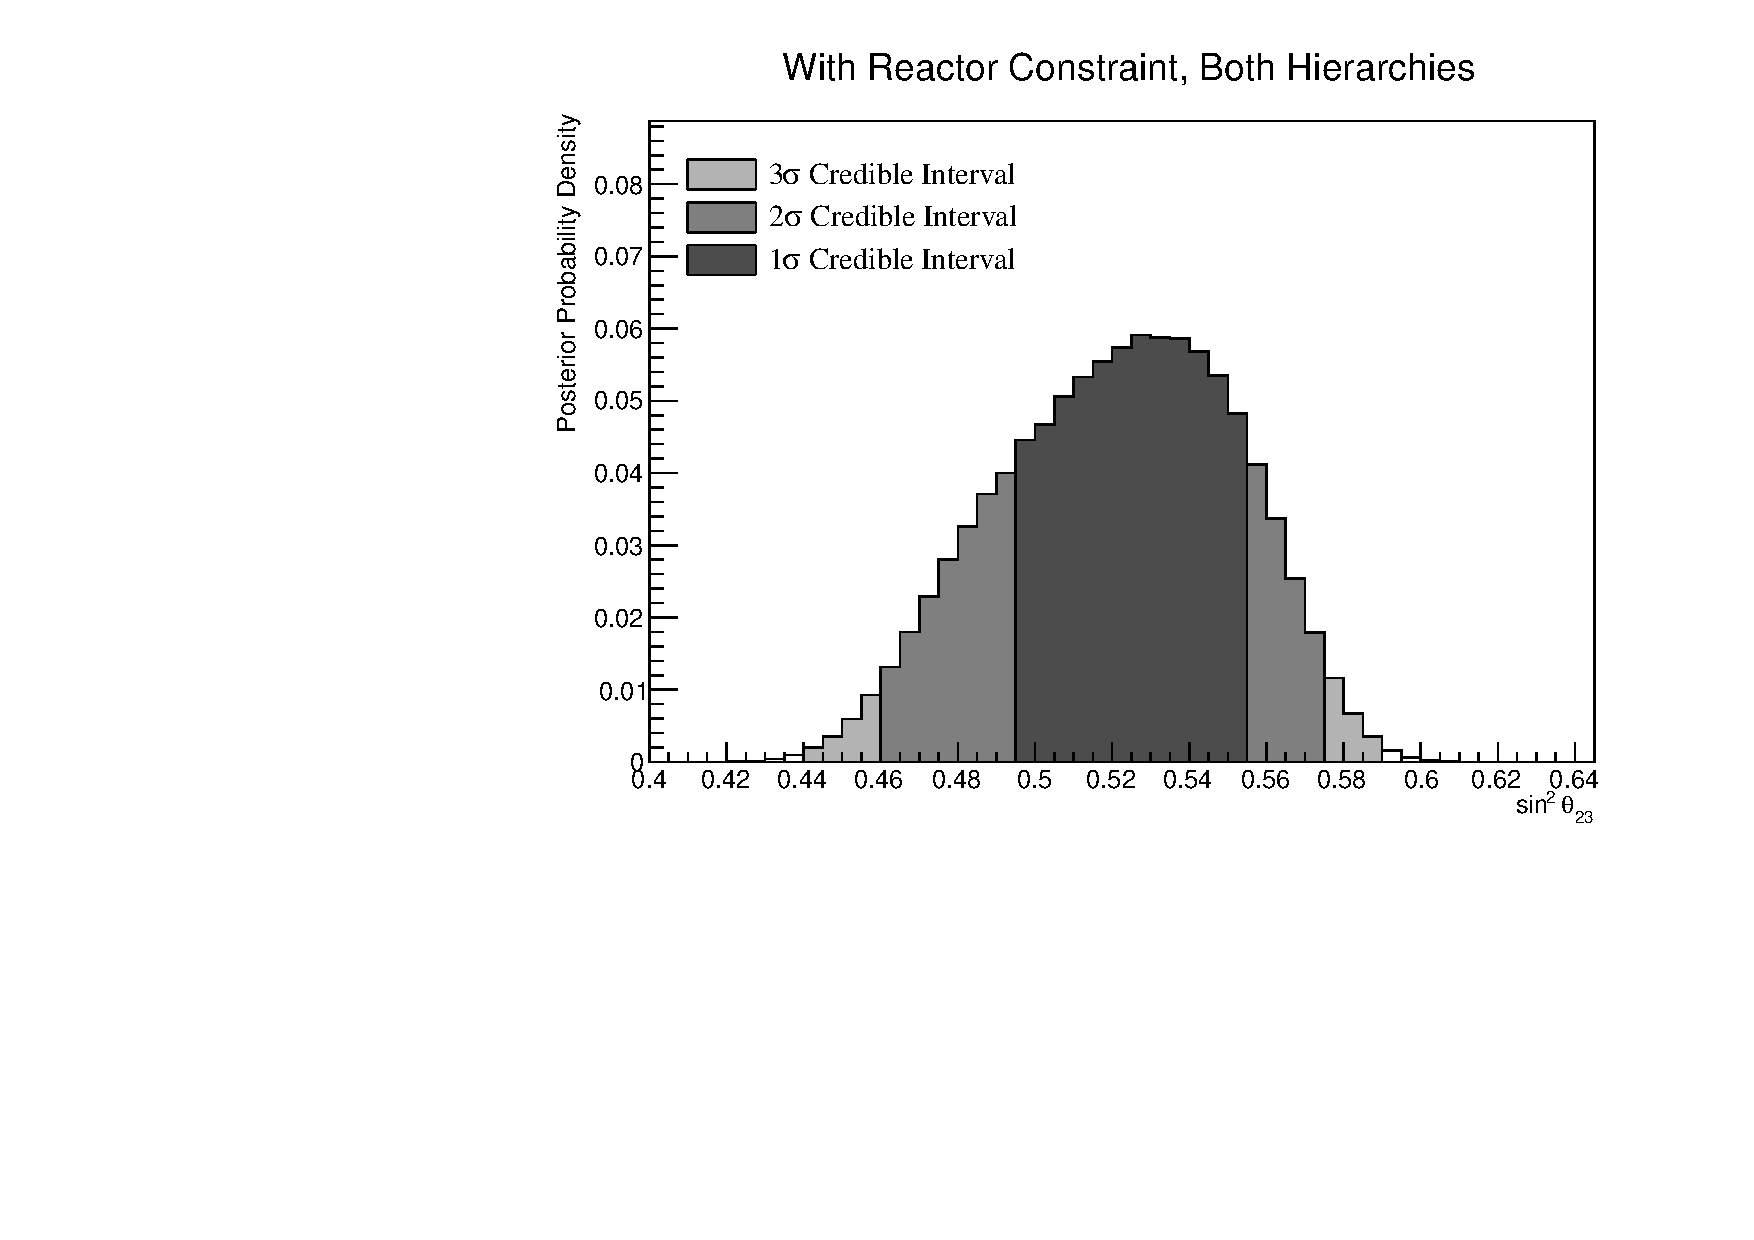
\includegraphics[width=\textwidth, trim={0mm 0mm 0mm 0mm}, clip,page=1]{Figures/OA/JointFit_wRC/Contours_1D_th23_BH_1_wRC_UnSmeared_CredibleInterval.pdf}
  \end{subfigure}
  \caption{The one-dimensional posterior probability density distribution in \quickmath{\sin^{2}(\theta_{23})}, marginalised over both hierarchies, from the joint beam-atmospheric fit where the reactor constraint is applied. The vertical dashed line represents the known value of \quickmath{\sin^{2}(\theta_{23})}.}
  \label{fig:OscillationAnalysis_JointFit_wRC_TH23}
\end{figure}

\begin{figure}[h]
  \begin{subfigure}[t]{0.98\textwidth}
    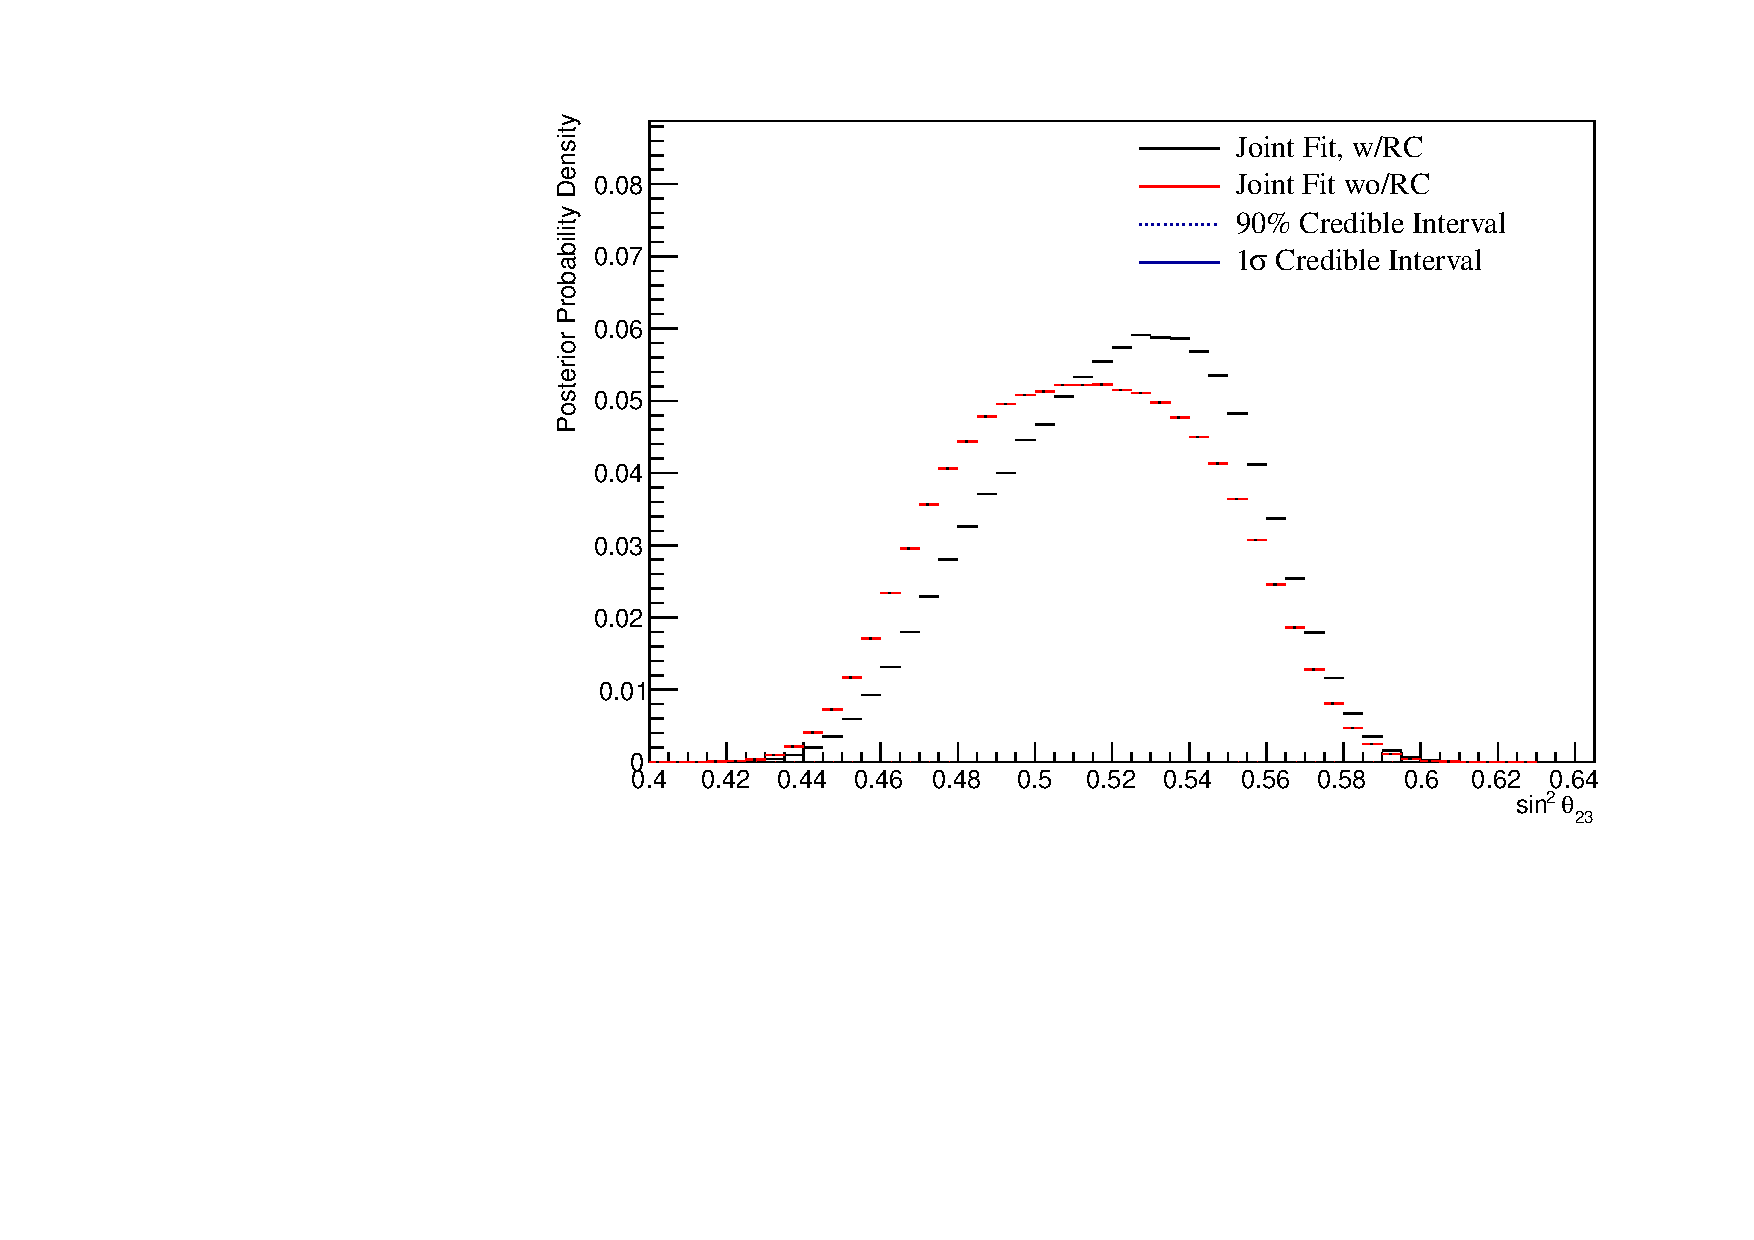
\includegraphics[width=\textwidth, trim={0mm 0mm 0mm 0mm}, clip,page=1]{Figures/OA/JointFit_wRC_Comp/ContourComparison_1D_th23_BH_2_wRC_woRC_UnSmeared_CredibleInterval.pdf}
  \end{subfigure}
  \caption{The one-dimensional posterior probability density distribution in \quickmath{\sin^{2}(\theta_{23})} compared between the joint beam-atmospheric fit (Red) and the joint beam-atmospheric fit with the reactor constraint (Black). The distributions are marginalised over both hierarchies. The vertical dashed line represents the known value of \quickmath{\sin^{2}(\theta_{23})}.}
  \label{fig:OscillationAnalysis_JointFit_wRC_Comp_TH23}
\end{figure}

The fraction of steps from the joint fit, after the reactor constraint is applied, is given in \autoref{tab:OscillationAnalysis_JointFit_BayesFactors_wRC} and split by the two hierarchy and two octant hypotheses. The reactor constraint significantly reduces the fraction of steps that are contained within the IH-LO region from \quickmath{0.08} to \quickmath{0.03}, whilst significantly increasing the fraction of steps within the NH-UO region from \quickmath{0.50} to \quickmath{0.62}. The application of the reactor constraint increases the Bayes factor from {B(\text{NH}/\text{IH}) = 3.67} to \quickmath{B(\text{NH}/\text{IH}) = 6.47}. There is a very clear preference for the correct hypothesis, with the Jeffreys scale stating a substantial preference for both fits. The Bayes factor for selecting the correct octant is calculated as \quickmath{B(\text{UO}/\text{LO}) = 2.64}. Whilst still a weak preference, this is certainly a stronger statement than the sensitivity when the reactor constraint is not applied.

\begin{table}[ht!]
  \centering
  \begingroup
  \renewcommand{\arraystretch}{1.5}
  \begin{tabular}{c|cc|c}
                                                        & LO \quickmath{\left(\sin^{2}\theta_{23} < 0.5 \right)} & UO \quickmath{\left( \sin^{2}\theta_{23} > 0.5 \right)} & Sum  \\ \hline
    NH \quickmath{\left( \Delta m^{2}_{32} > 0 \right)} &                                                   0.24 &                                                    0.62 & 0.87 \\
    IH \quickmath{\left( \Delta m^{2}_{32} < 0 \right)} &                                                   0.03 &                                                    0.10 & 0.13 \\ \hline
    Sum                                                 &                                                   0.27 &                                                    0.73 & 1.00 \\
  \end{tabular}
  \caption{The distribution of steps in a joint beam-atmospheric with the reactor constraint fit applied, presented as the fraction of steps in the upper (UO) and lower (LO) octants and the normal (NH) and inverted (IH) hierarchies. The Bayes factors are calculated as \quickmath{B(\text{NH}/\text{IH}) = 6.47} and \quickmath{B(\text{UO}/\text{LO}) = 2.64}.}
  \label{tab:OscillationAnalysis_JointFit_BayesFactors_wRC}
  \endgroup
\end{table}

The sensitivity of the joint beam-atmospheric fit to \quickmath{\Delta m^{2}_{32}}, with the reactor constraint applied, is presented in \autoref{fig:OscillationAnalysis_JointFit_wRC_DM32}.
%The posterior distribution is marginalised over both hierarchies.
The \quickmath{1\sigma} credible interval is entirely contained within the NH region and the position of the highest posterior probability density is given as \quickmath{(2.49 \pm 0.01) \times 10^{-3} \text{eV}^{2}}. This illustrates no bias between the fit results and the known oscillation parameters. The application of the reactor constraint does not significantly move the position or width of the credible intervals.

\begin{figure}[h]
  \begin{subfigure}[t]{0.98\textwidth}
    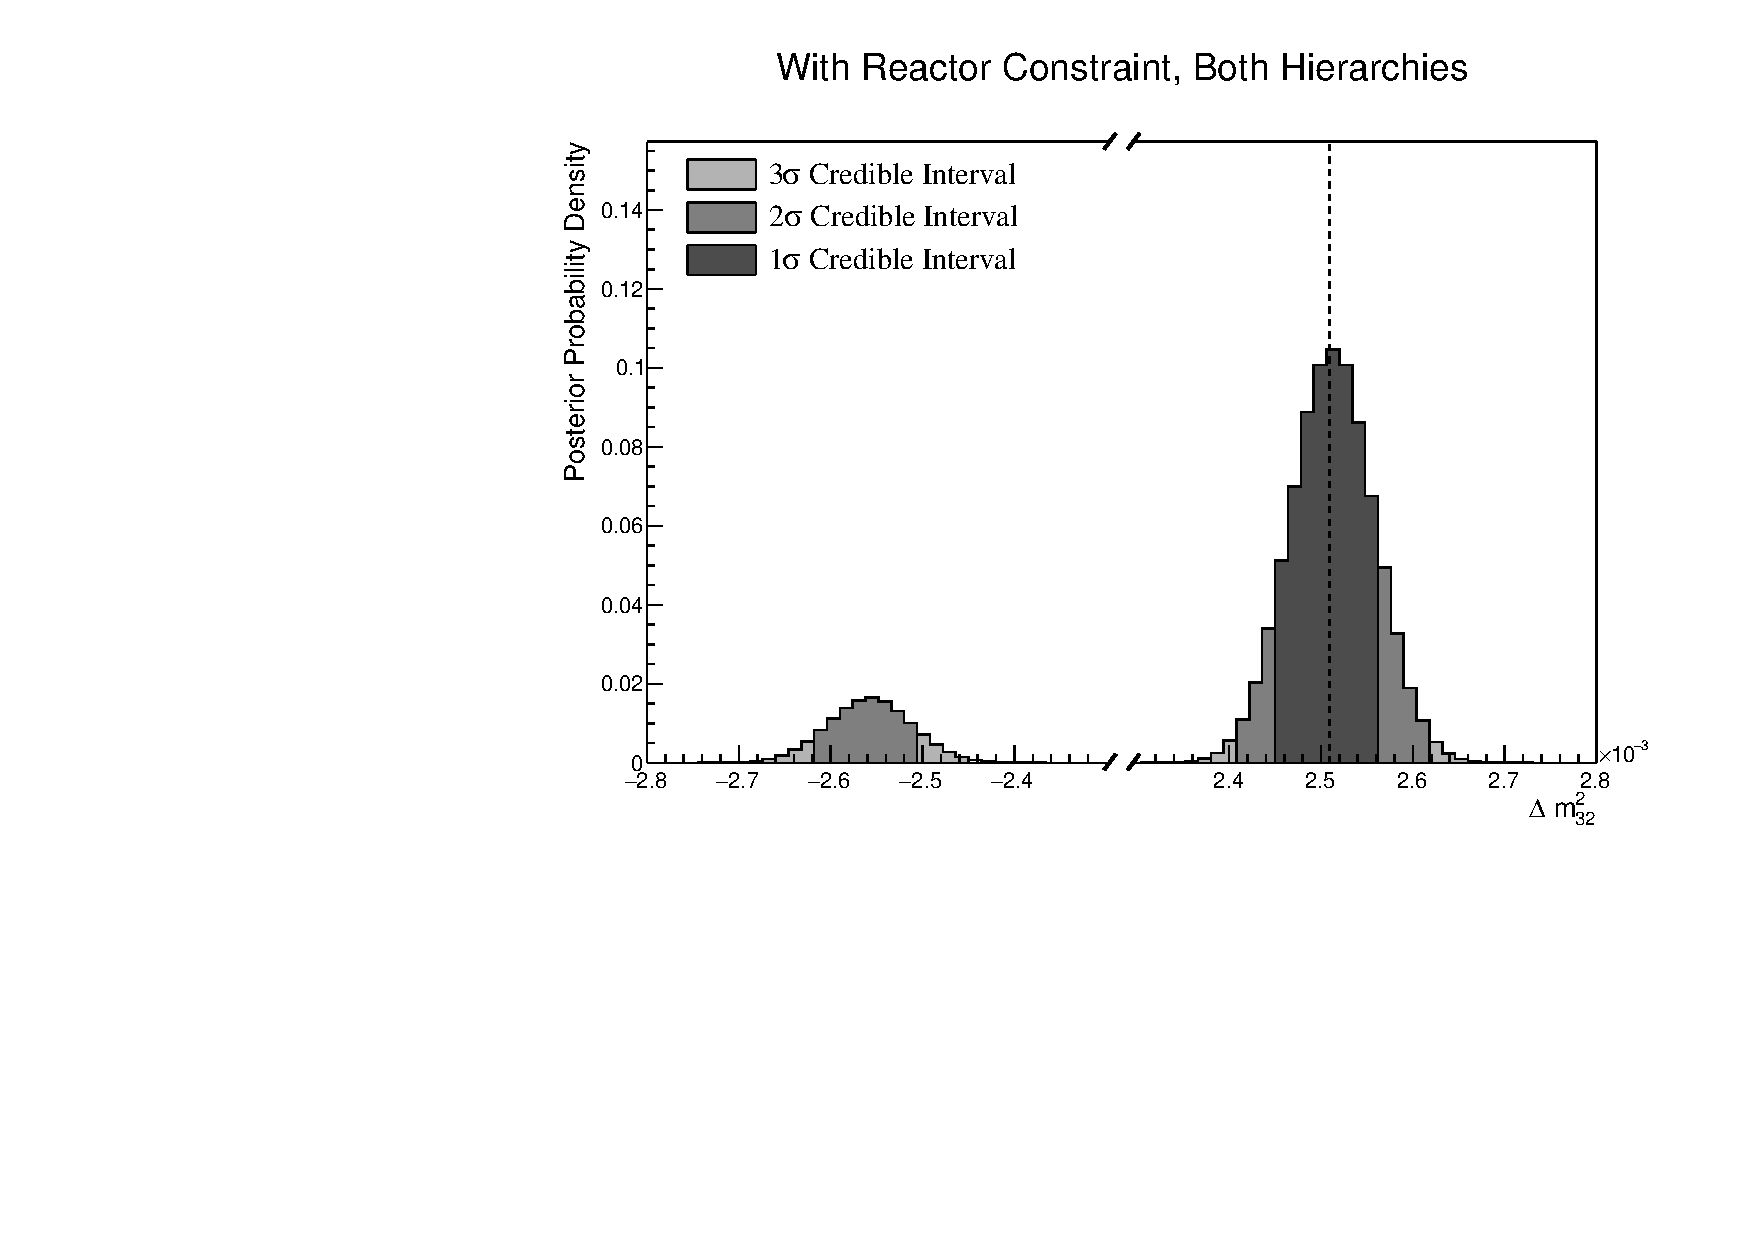
\includegraphics[width=\textwidth, trim={0mm 0mm 0mm 0mm}, clip,page=1]{Figures/OA/JointFit_wRC/Contours_1D_dm32_BH_1_wRC_UnSmeared_CredibleInterval.pdf}
  \end{subfigure}
  \caption{The one-dimensional posterior probability density distribution in \quickmath{\Delta m^{2}_{32}} from the joint beam-atmospheric fit where the reactor constraint is applied. The vertical dashed line represents the known value of \quickmath{\Delta m^{2}_{32}}.}
  \label{fig:OscillationAnalysis_JointFit_wRC_DM32}
\end{figure}

\begin{figure}[h]
  \begin{subfigure}[t]{0.98\textwidth}
    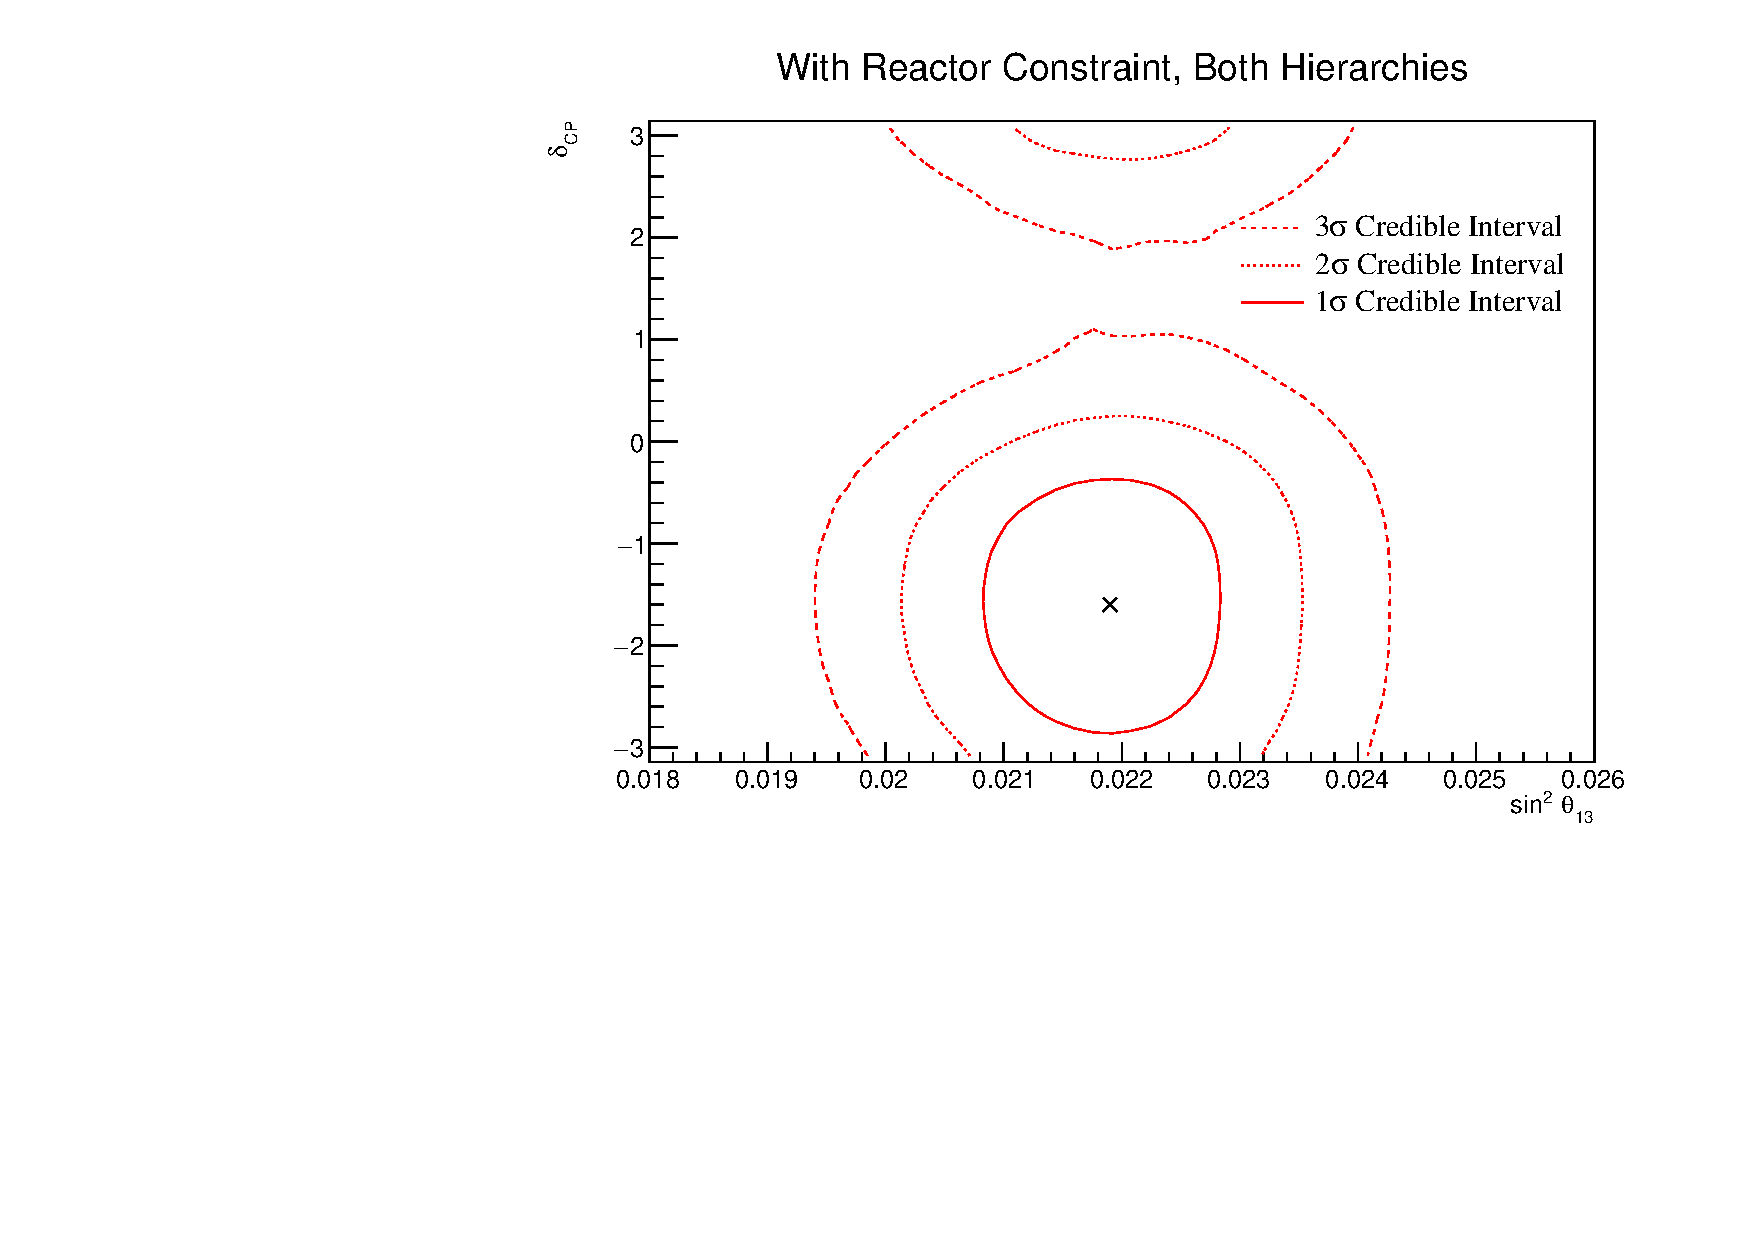
\includegraphics[width=\textwidth, trim={0mm 0mm 0mm 0mm}, clip,page=1]{Figures/OA/JointFit_wRC/Contours_2D_th13_dcp_BH_1_wRC_UnSmeared_CredibleInterval.pdf}
  \end{subfigure}
  \caption{The two-dimensional posterior probability density distribution in \quickmath{\delta_{CP}-\sin^{2}(\theta_{13})}, marginalised over both hierarchies, from the joint beam-atmospheric fit where the reactor constraint is applied. The marker represents the known value of \quickmath{\delta_{CP}-\sin^{2}(\theta_{13})}.}
  \label{fig:OscillationAnalysis_JointFit_wRC_TH13DCP}
\end{figure}

\begin{figure}[h]
  \begin{subfigure}[t]{0.98\textwidth}
    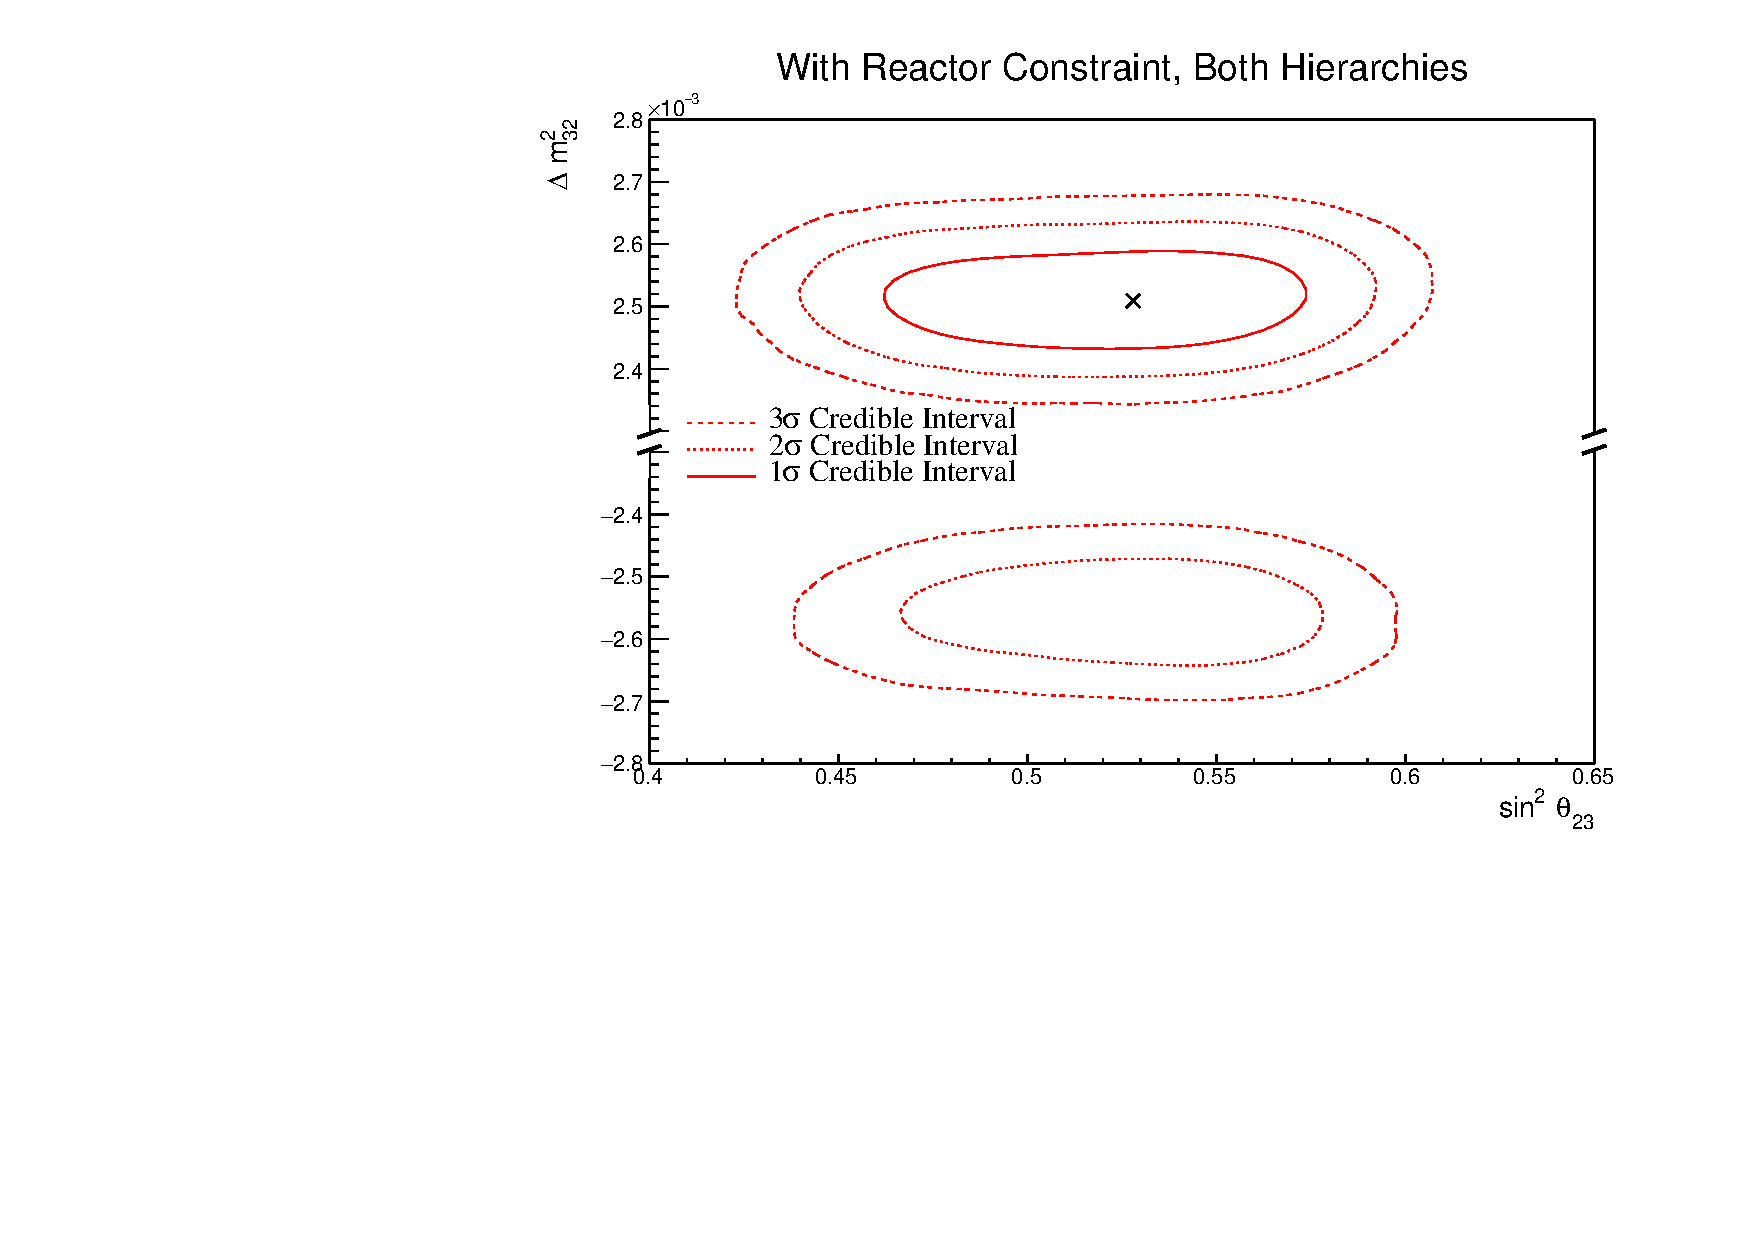
\includegraphics[width=\textwidth, trim={0mm 0mm 0mm 0mm}, clip,page=1]{Figures/OA/JointFit_wRC/Contours_2D_th23_dm32_BH_1_wRC_UnSmeared_CredibleInterval.pdf}
  \end{subfigure}
  \caption{The two-dimensional posterior probability density distribution in \quickmath{\Delta m^{2}_{32}-\sin^{2}(\theta_{23})}, marginalised over both hierarchies, from the joint beam-atmospheric fit where the reactor constraint is applied. The marker represents the known value of \quickmath{\Delta m^{2}_{32}-\sin^{2}(\theta_{23})}.}
  \label{fig:OscillationAnalysis_JointFit_wRC_TH23DM32}
\end{figure}

The sensitivity to the appearance parameters (\quickmath{\sin^{2}(\theta_{13})\text{\textendash}\delta_{CP}}) is given in \autoref{fig:OscillationAnalysis_JointFit_wRC_TH13DCP}. The distribution is mostly uncorrelated between the two parameters and is centered at the known oscillation parameters. The \quickmath{1\sigma} credible interval excludes \quickmath{\delta_{CP} = 0} and \quickmath{\delta_{CP} = \pm\pi}. Furthermore, the \quickmath{3\sigma} credible intervals exclude the region of \quickmath{\delta_{CP} = \pi/2}.

The sensitivity to the disappearance parameters (\quickmath{\sin^{2}(\theta_{23})\text{\textendash}\Delta m^{2}_{32}}) is illustrated in \autoref{fig:OscillationAnalysis_JointFit_wRC_TH23DM32}. The \quickmath{1\sigma} credible interval is entirely contained within the NH region reflecting the same results as the one-dimensional marginalised results in \autoref{fig:OscillationAnalysis_JointFit_wRC_DM32}. Both the NH and IH regions favour the UO, with a visually similar preference in both hierarchies. The width of the \quickmath{1\sigma} contour, in \quickmath{\Delta m^{2}_{32}}, does not significantly depend upon the value or octant of \quickmath{\sin^{2}(\theta_{23})}. This shows that there are no strong correlations between these two parameters.

\autoref{fig:OscillationAnalysis_JointFit_wRC_TrianglePlot} illustrates the posterior distribution for each permutation of two oscillation parameters of interest. The application of the reactor constraint significantly reduces the correlations previously seen in \autoref{fig:OscillationAnalysis_JointFit_TriPlot}.
%There is still a small correlation between \quickmath{\delta_{CP}} and \quickmath{\Delta m^{2}_{32}}. The application of the reactor constraint has not significantly affected this correlation. The width of the \quickmath{1\sigma} credible interval in \quickmath{\Delta m^{2}_{32}} is wider for a value of \quickmath{\delta_{CP} = 0} compared to a value of \quickmath{\delta_{CP} = \pi}. Similarly, the width of the \quickmath{1\sigma} credible interval in \quickmath{\delta_{CP}} is smaller for lower values of \quickmath{\sin^{2}(\theta_{23})}.

\begin{figure}[h]
  \begin{subfigure}[t]{0.98\textwidth}
    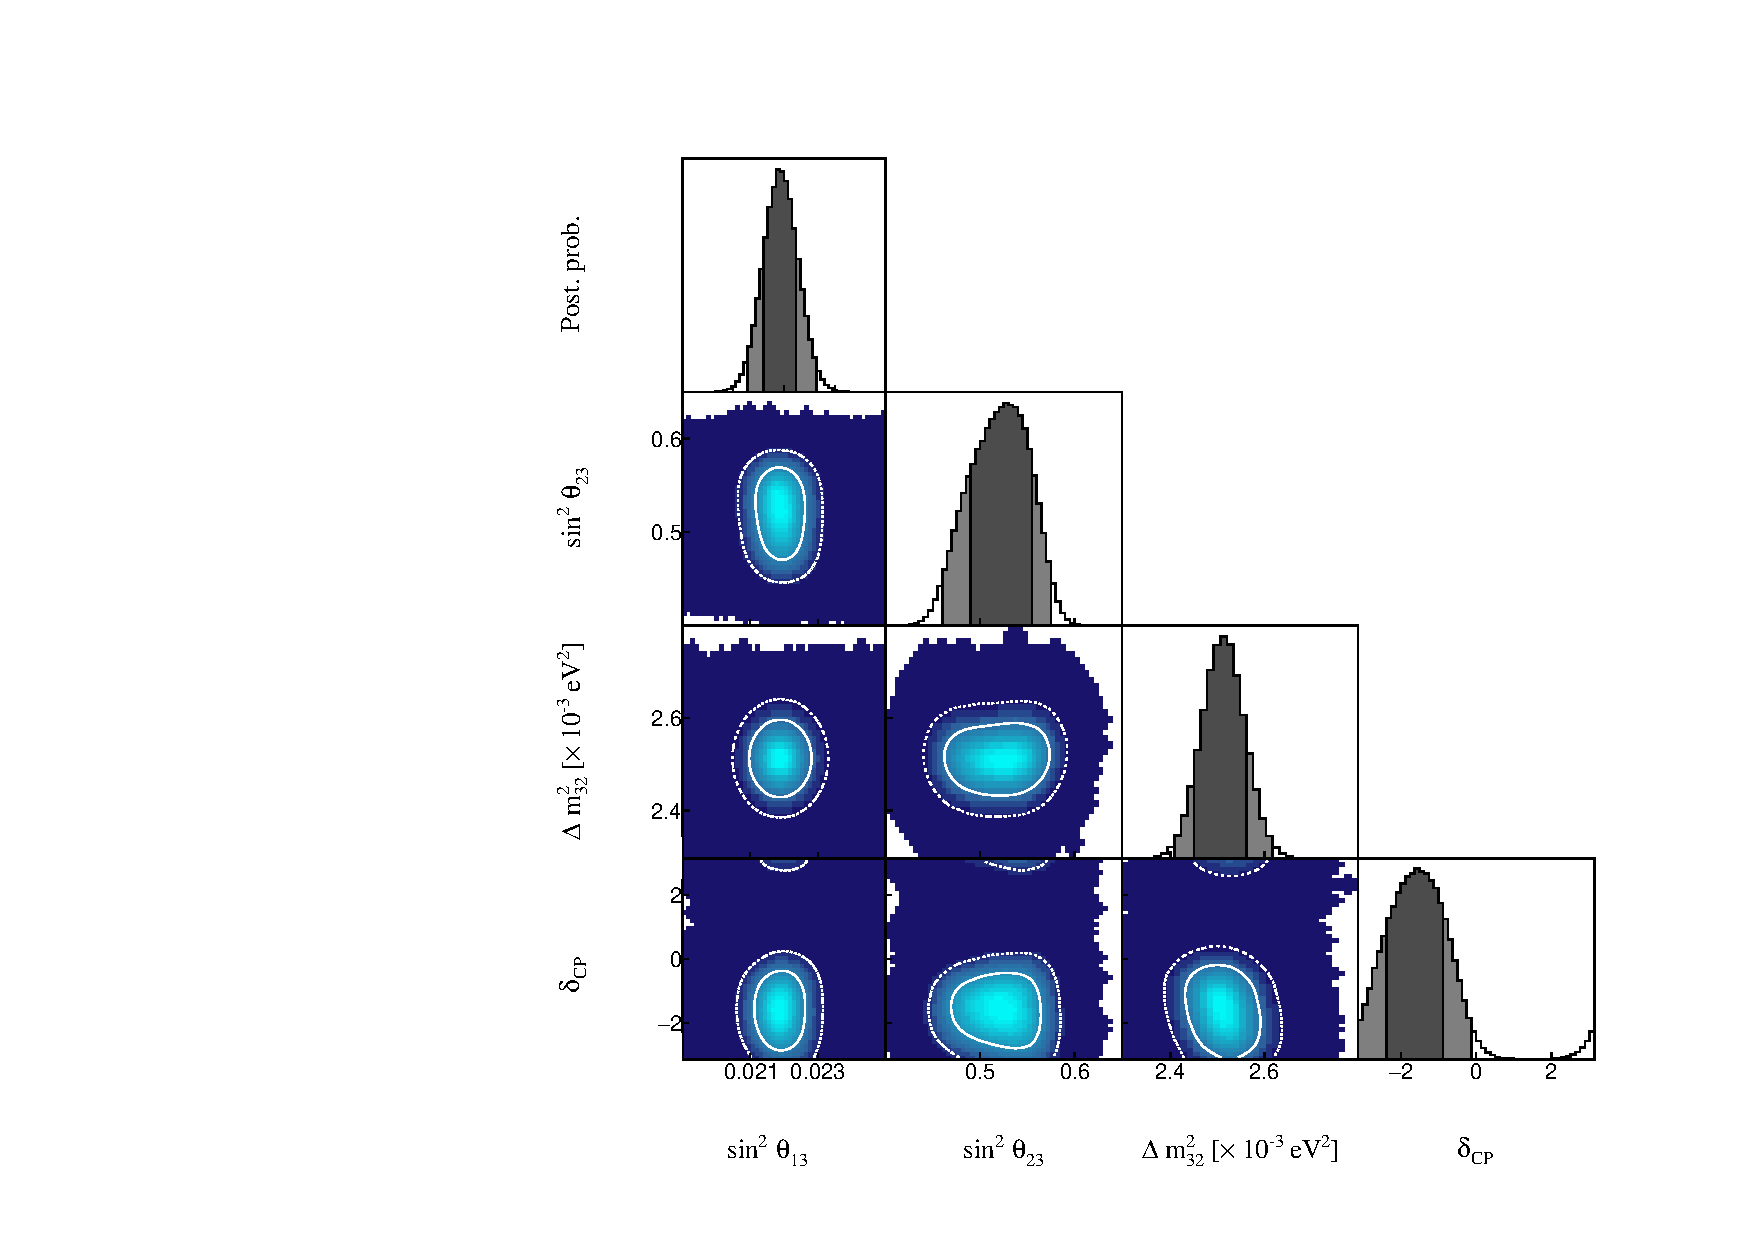
\includegraphics[width=\textwidth, trim={0mm 0mm 0mm 0mm}, clip,page=1]{Figures/OA/JointFit_wRC/Contours_1D_wRC_UnSmeared_CredibleInterval_TrianglePlot.pdf}
  \end{subfigure}
  \caption{The posterior probability density distribution from the joint beam-atmospheric fit where the reactor constraint is applied. The distribution is given for each two-dimensional permutation of the oscillation parameters of interest. The one-dimensional distribution of each parameter is also given.}
  \label{fig:OscillationAnalysis_JointFit_wRC_TrianglePlot}
\end{figure}

\clearpage
\subsection{Comparison to Latest T2K Sensitivities without Reactor Constraint}
\label{sec:OscillationAnalysis_JointFit_OA2020}

The benefits of the joint beam-atmospheric analysis can be determined by comparing the sensitivities to the beam-only analysis presented in \cite{Dunne2020-uf, t2k_tn_393}. This section presents those comparisons for sensitivities built using the Asimov A oscillation parameters defined in \autoref{tab:Theory_ParameterSets} and the post-BANFF systematic tune. The reactor constraint is not applied within either of the fits used in these comparisons.

\begin{figure}[h]
  \begin{subfigure}[t]{0.98\textwidth}
    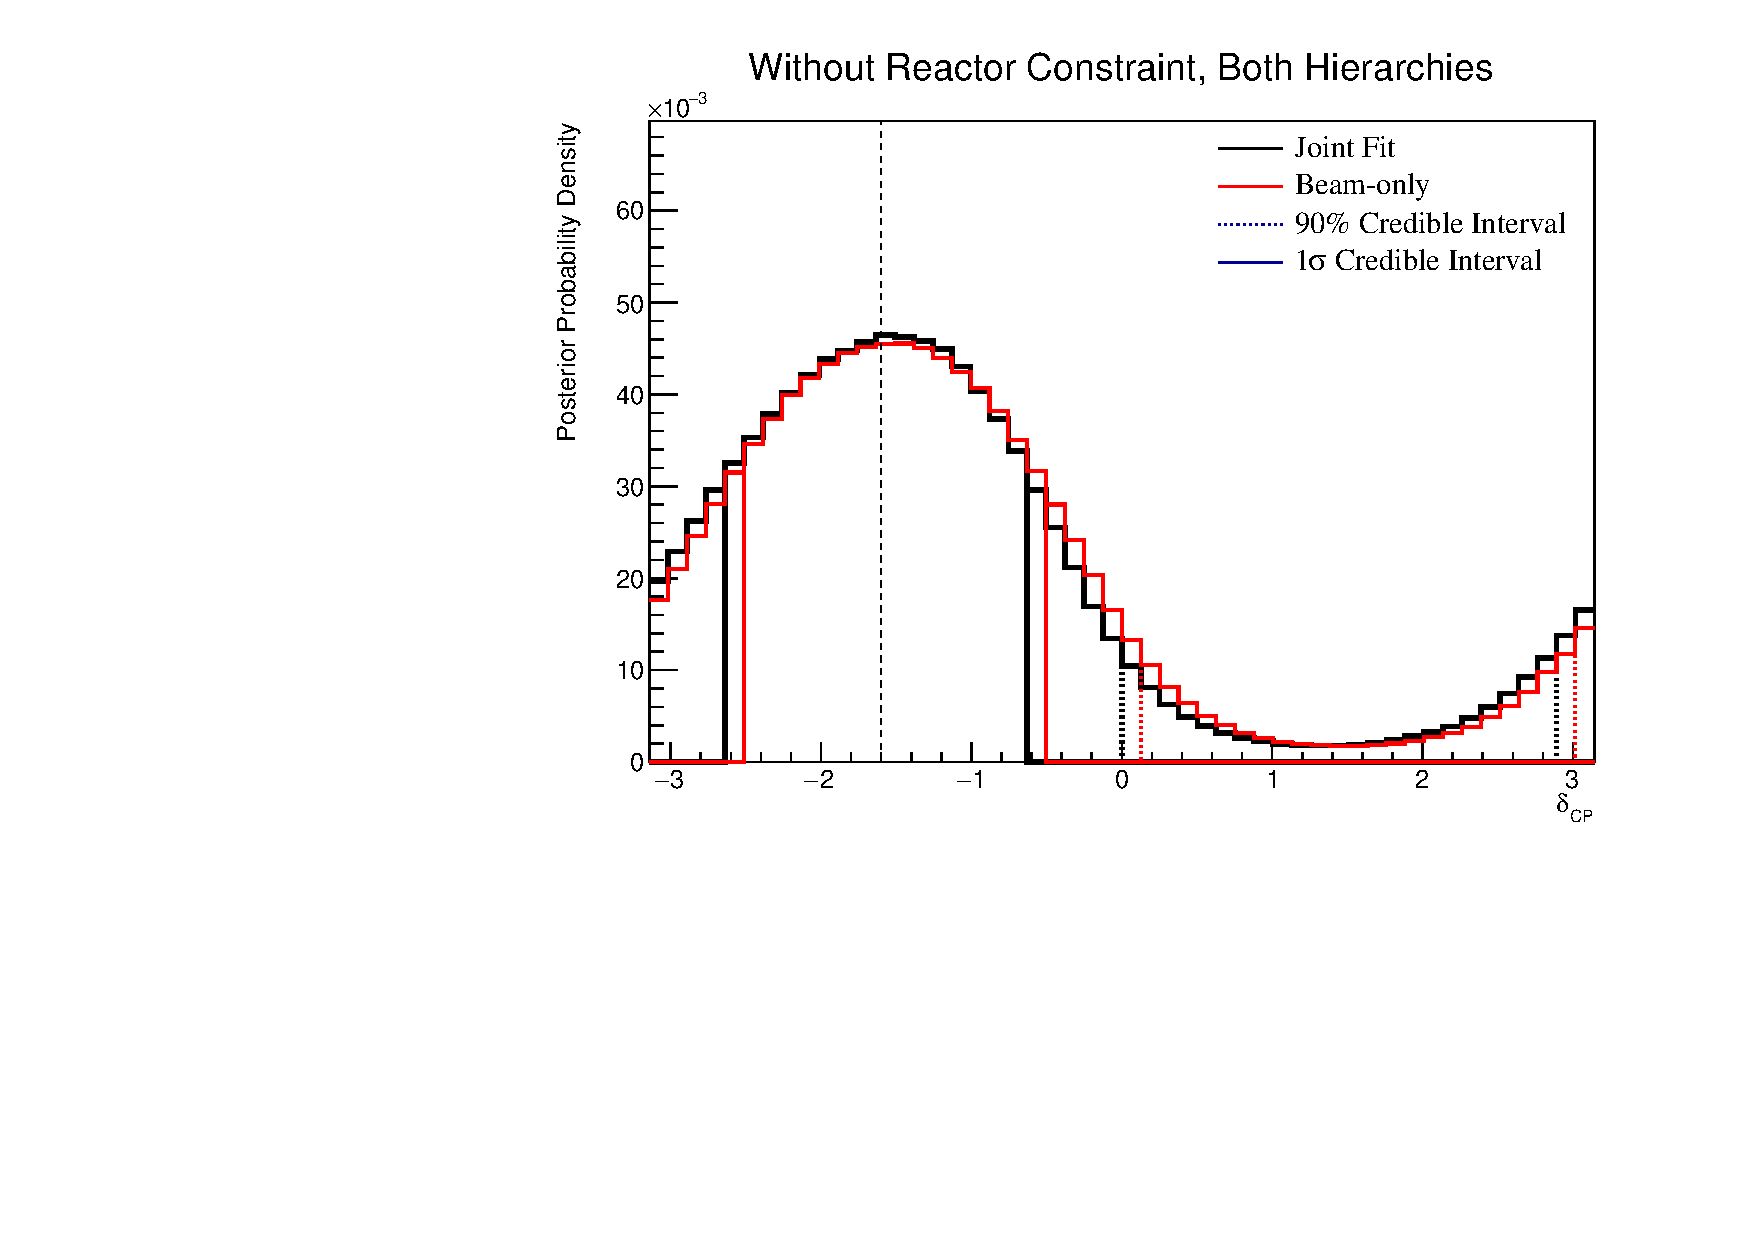
\includegraphics[width=\textwidth, trim={0mm 0mm 0mm 0mm}, clip,page=1]{Figures/OA/JointFit_OA2020_Comp/ContourComparison_1D_dcp_BH_2_woRC_UnSmeared_CredibleInterval.pdf}
  \end{subfigure}
  \caption{The one-dimensional posterior probability density distribution in \quickmath{\delta_{CP}} compared between the joint beam-atmospheric fit (Black) and the latest T2K sensitivities (Red) \cite{Dunne2020-uf, t2k_tn_393}. The reactor constraint is not applied in either fit. The distributions are marginalised over both hierarchies. The vertical dashed line represents the known value of \quickmath{\delta_{CP}}.}
  \label{fig:OscillationAnalysis_JointFit_OA2020_DCP}
\end{figure}

The sensitivity, marginalised over both hierarchies, to \quickmath{\delta_{CP}} from the joint beam-atmospheric and beam-only fits is presented in \autoref{fig:OscillationAnalysis_JointFit_OA2020_DCP}. As expected from the likelihood scans (\autoref{fig:OscillationAnalysis_AsimovEval_DCP}), the sensitivity to \quickmath{\delta_{CP}} is not significantly increased. This is because the known oscillation parameter value lies at the position where the beam samples dominate the sensitivity compared to the SK samples.

The sensitivity to \quickmath{\Delta m^{2}_{32}} is compared between the joint beam-atmospheric fit and beam-only fit in \autoref{fig:OscillationAnalysis_JointFit_OA2020_DM32}. The \quickmath{1\sigma} credible interval of the joint beam-atmospheric fit is entirely contained within the NH region. This shows the significant increase in the ability of the fit to determine the correct mass hierarchy, compared to the beam-only analysis. This is further evidenced by the fact that the \quickmath{90\%} credible intervals from the joint fit are also tighter in the IH region compared to the beam-only analysis. The Bayes factor for mass hierarchy determination for the beam-only and joint beam-atmospheric fits are \quickmath{B(\text{NH}/\text{IH}) = 1.91} and \quickmath{B(\text{NH}/\text{IH}) = 3.67}, respectively. According to Jeffrey's scale, the beam-only analysis represents a weak preference for the correct hierarchy whereas the joint fit returns a substantial preference for the NH hypothesis. Notably, this conclusion does not require any external constraints and clearly illustrates the benefit of the joint analysis.
%To summarise, the joint beam-atmospheric fit has a substantial preference for the correct hierarchy without the requirement of external constraints.

\begin{figure}[h]
  \begin{subfigure}[t]{0.98\textwidth}
    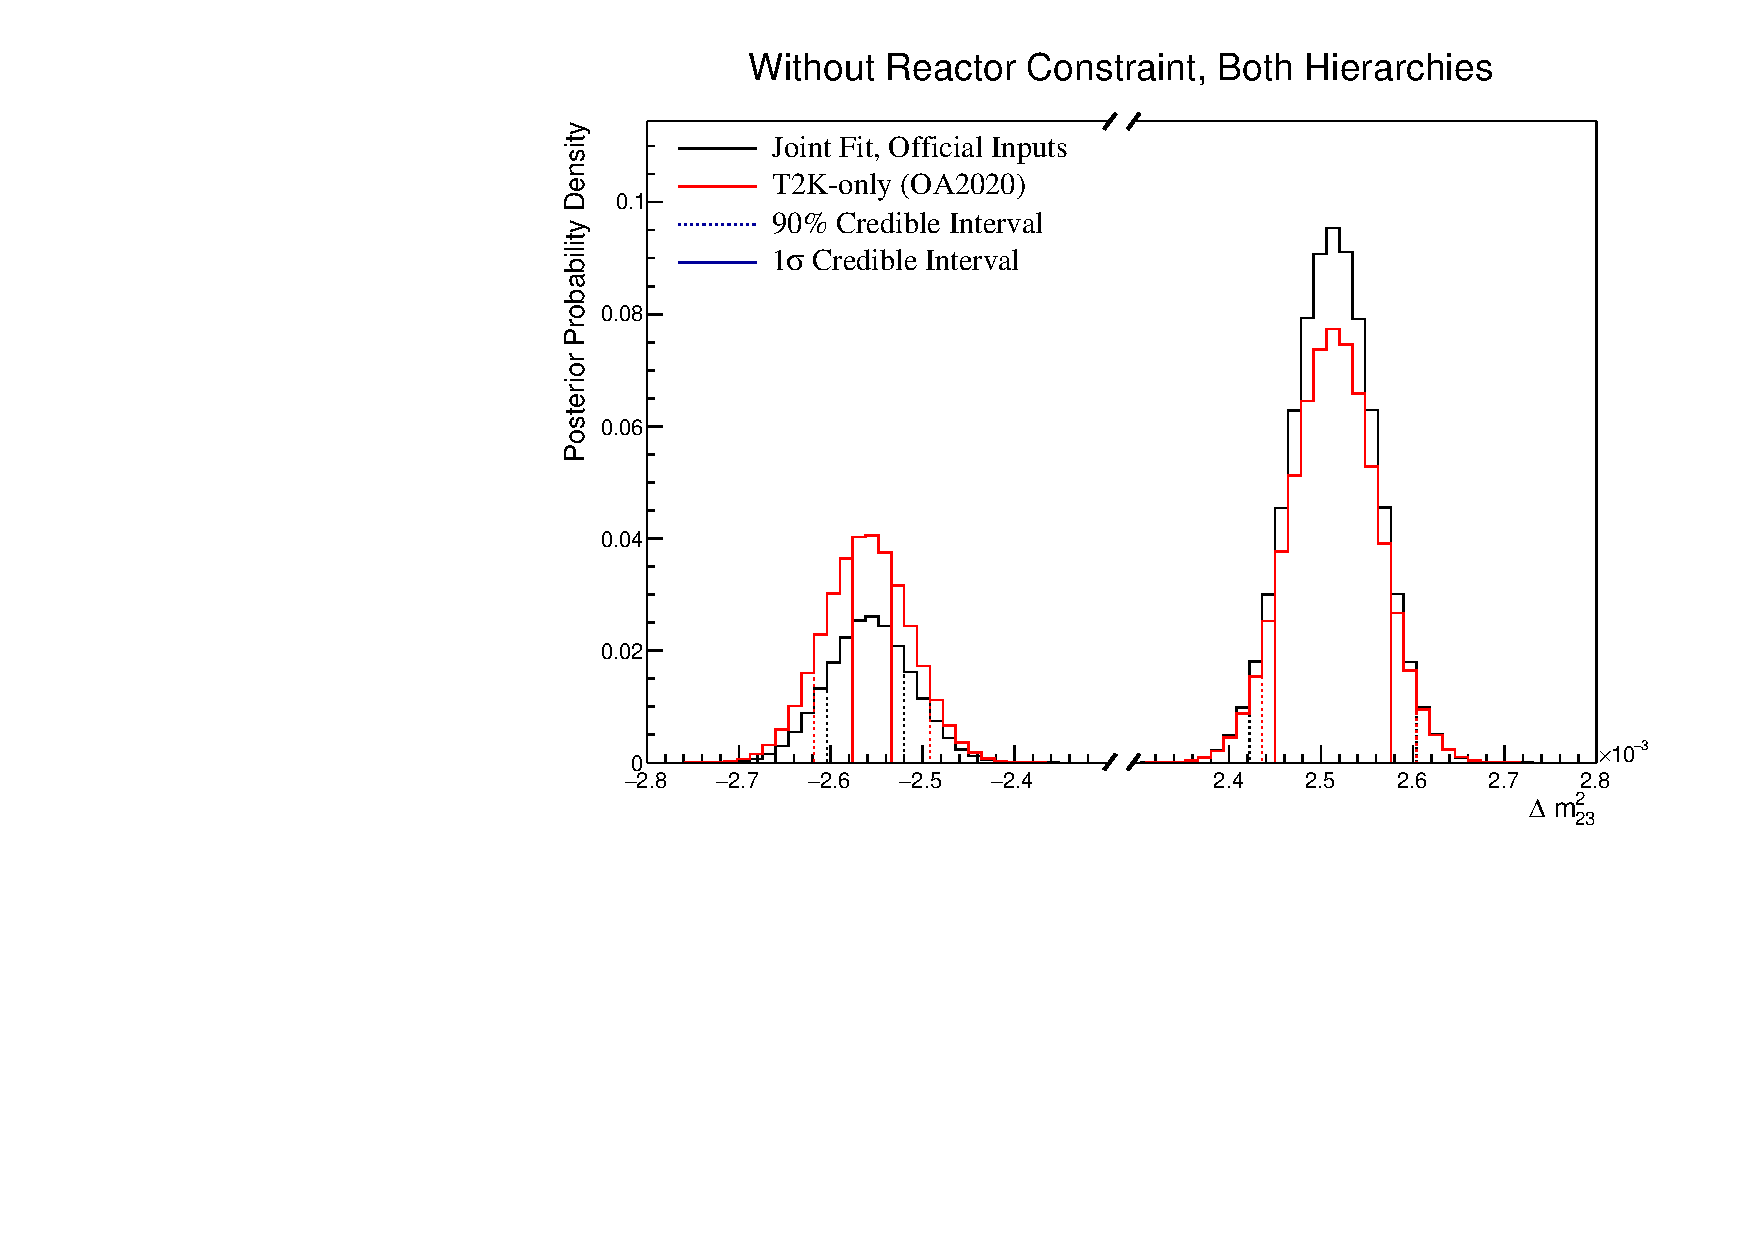
\includegraphics[width=\textwidth, trim={0mm 0mm 0mm 0mm}, clip,page=1]{Figures/OA/JointFit_OA2020_Comp/ContourComparison_1D_dm32_BH_2_woRC_UnSmeared_CredibleInterval.pdf}
  \end{subfigure}
  \caption{The one-dimensional posterior probability density distribution in \quickmath{\Delta m^{2}_{32}} compared between the joint beam-atmospheric fit (Black) and the latest T2K sensitivities (Red) \cite{Dunne2020-uf, t2k_tn_393}. The reactor constraint is not applied in either fit. The vertical dashed line represents the known value of \quickmath{\Delta m^{2}_{32}}.}
  \label{fig:OscillationAnalysis_JointFit_OA2020_DM32}
\end{figure}

The sensitivity to \quickmath{\sin^{2}(\theta_{23})}, marginalised over both hierarchies, for both the beam-only and joint beam-atmospheric analysis are presented in \autoref{fig:OscillationAnalysis_JointFit_OA2020_TH23}. The peak of the posterior distribution from the joint analysis is more aligned with the known value of \quickmath{\sin^{2}(\theta_{23}) = 0.528} compared to the beam-only analysis.
%This indicates that the marginalisation effects from other oscillation parameters (\quickmath{\sin^{2}(\theta_{13})\text{\textendash}\sin^{2}(\theta_{23})} presented in \autoref{fig:OscillationAnalysis_JointFit_TriPlot}) are less prevalent in the projection of this parameter.
%Furthermore, the width of the credible intervals are marginally smaller, so this change would not affect any conclusion one would make about the parameter sensitivity.
The Bayes factors for the beam-only and joint beam-atmospheric fit are \quickmath{B(\text{UO}/\text{LO}) = 1.56} and \quickmath{B(\text{UO}/\text{LO}) = 1.74}, respectively. Therefore, the joint beam-atmospheric fit does prefer the UO more strongly than the beam-only analysis, albeit slightly.

\begin{figure}[h]
  \begin{subfigure}[t]{0.98\textwidth}
    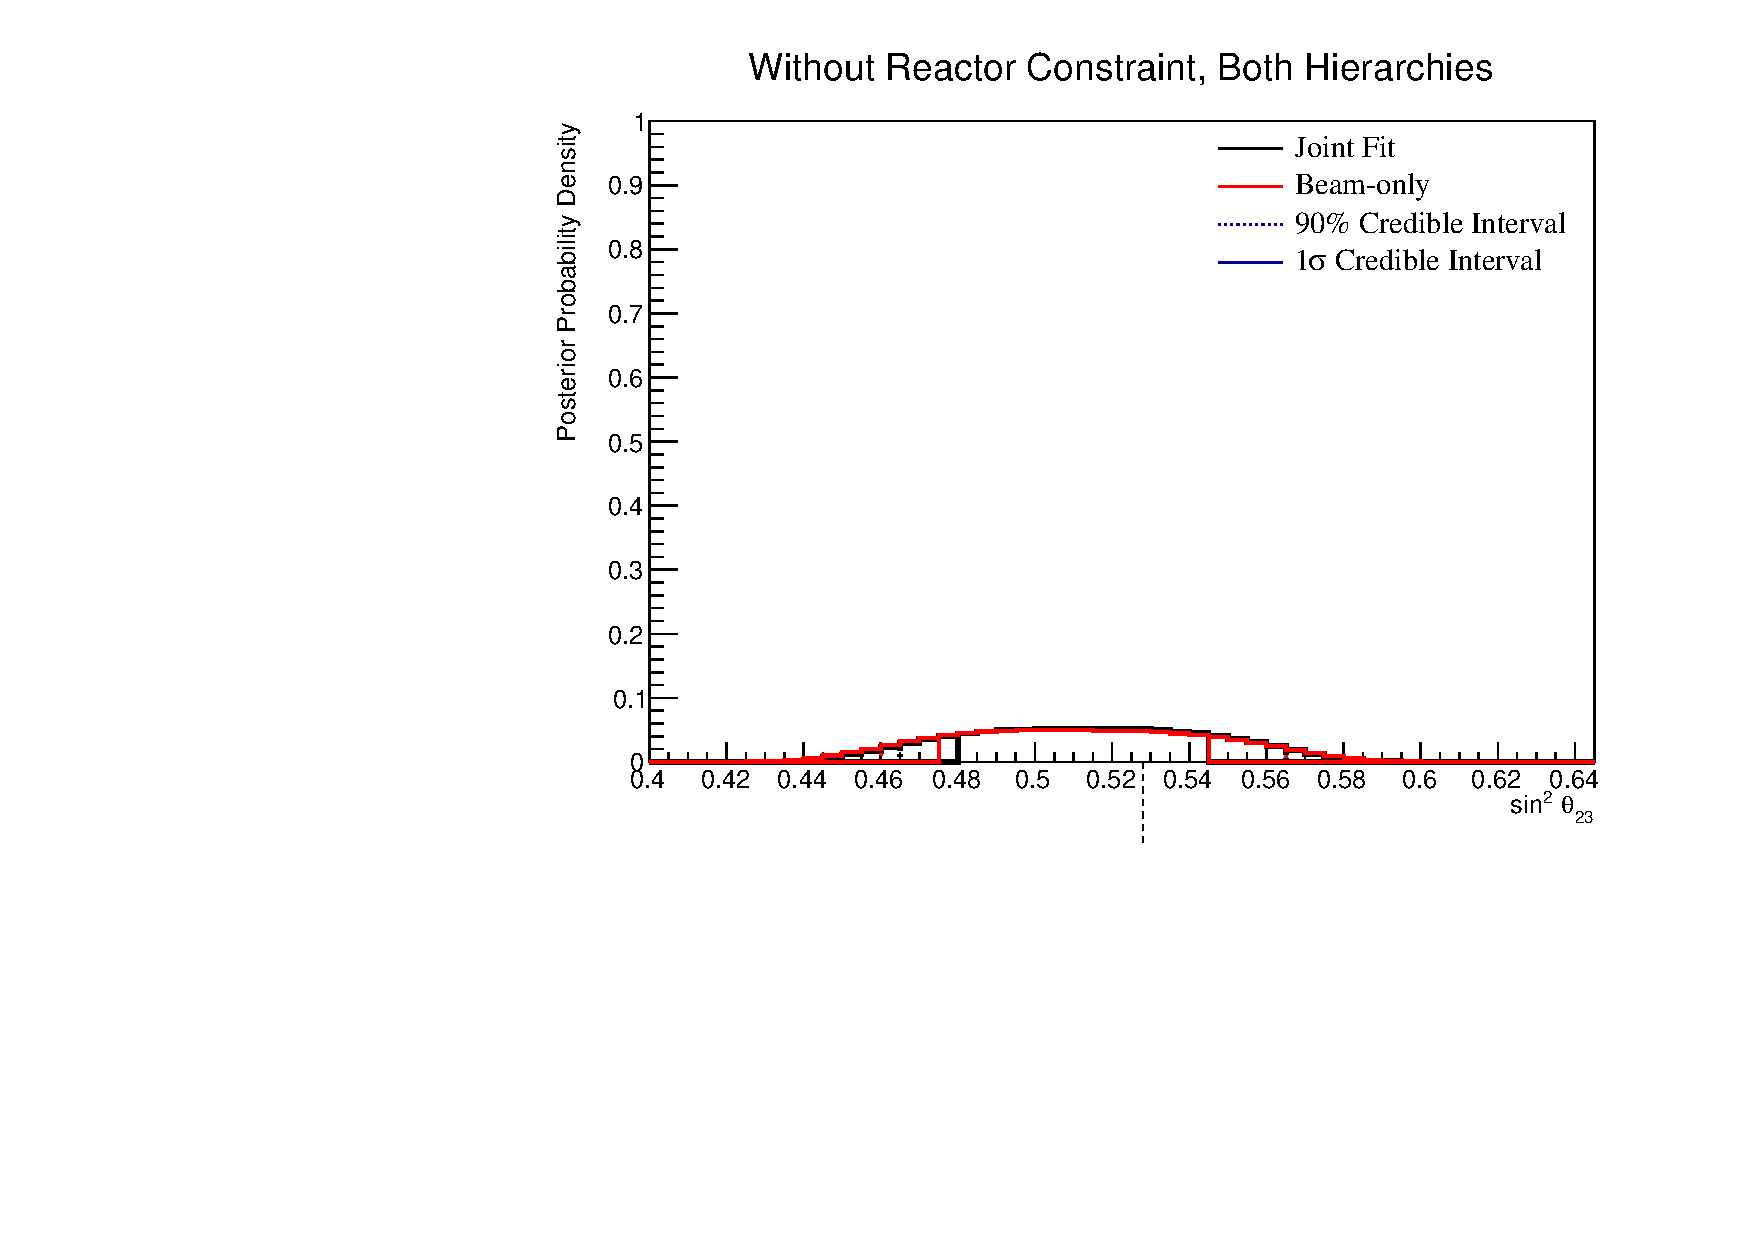
\includegraphics[width=\textwidth, trim={0mm 0mm 0mm 0mm}, clip,page=1]{Figures/OA/JointFit_OA2020_Comp/ContourComparison_1D_th23_BH_2_woRC_UnSmeared_CredibleInterval.pdf}
  \end{subfigure}
  \caption{The one-dimensional posterior probability density distribution in \quickmath{\sin^{2}(\theta_{23})} compared between the joint beam-atmospheric fit (Black) and the latest T2K sensitivities (Red) \cite{Dunne2020-uf, t2k_tn_393}. The reactor constraint is not applied in either fit. The distributions are marginalised over both hierarchies. The vertical dashed line represents the known value of \quickmath{\sin^{2}(\theta_{23})}.}
  \label{fig:OscillationAnalysis_JointFit_OA2020_TH23}
\end{figure}

Whilst the beam-only and joint beam-atmospheric fits have similar sensitivity to \quickmath{\delta_{CP}} and \quickmath{\sin^{2}(\theta_{23})} when projected in one-dimension, the benefit of the joint analysis becomes more obvious when the sensitivities are presented in two-dimensions. The sensitivity of the two fits to the appearance parameters (\quickmath{\delta_{CP}\text{\textendash}\sin^{2}(\theta_{13})}) is illustrated in \autoref{fig:OscillationAnalysis_JointFit_OA2020_DCPTH13}. The width of the \quickmath{99\%} joint fit credible interval in \quickmath{\sin^{2}(\theta_{13})} is squeezed in the region of \quickmath{\delta_{CP} \sim 0} compared to the beam-only analysis. This is the same behaviour that is seen in the appearance likelihood scans presented in \autoref{fig:OscillationAnalysis_2DLLHOscScans_App}. The \quickmath{1\sigma} and \quickmath{90\%} also exhibit slightly tighter constraints on \quickmath{\delta_{CP}}. This is most prevalent in the region of \quickmath{\delta_{CP} \sim 0} and \quickmath{\sin^{2}(\theta_{13}) \sim 0.03}. Whilst the atmospheric samples do not have significant sensitivity to \quickmath{\sin^{2}(\theta_{13})} (as shown in \autoref{fig:OscillationAnalysis_LLHScanOscPars}), they aid in breaking the degeneracy between the oscillation parameters allowing for tighter constraints.

The sensitivity to the disappearance parameters \quickmath{\sin^{2}(\theta_{23})\text{\textendash}\Delta m^{2}_{32}} is presented in \autoref{fig:OscillationAnalysis_JointFit_OA2020_DM32TH23} for both the beam-only and joint beam-atmospheric fits. Whilst the one-dimensional sensitivity comparisons considered so far show the improvements of the joint fit, the two-dimensional projection really shows the benefit of adding the atmospheric samples to the beam samples. The area contained within the IH credible intervals is drastically reduced in the joint fit. This follows from the better determination of the mass hierarchy seen in the Bayes factor comparisons.
%The \quickmath{1\sigma} joint fit credible interval in the IH region more strongly favours the UO compared to the beam-only fit.
Even in the NH region, the widths of the credible intervals in \quickmath{\sin^{2}(\theta_{23})} decreases, albeit to a smaller extent.

\begin{figure}[h]
  \begin{subfigure}[t]{0.98\textwidth}
    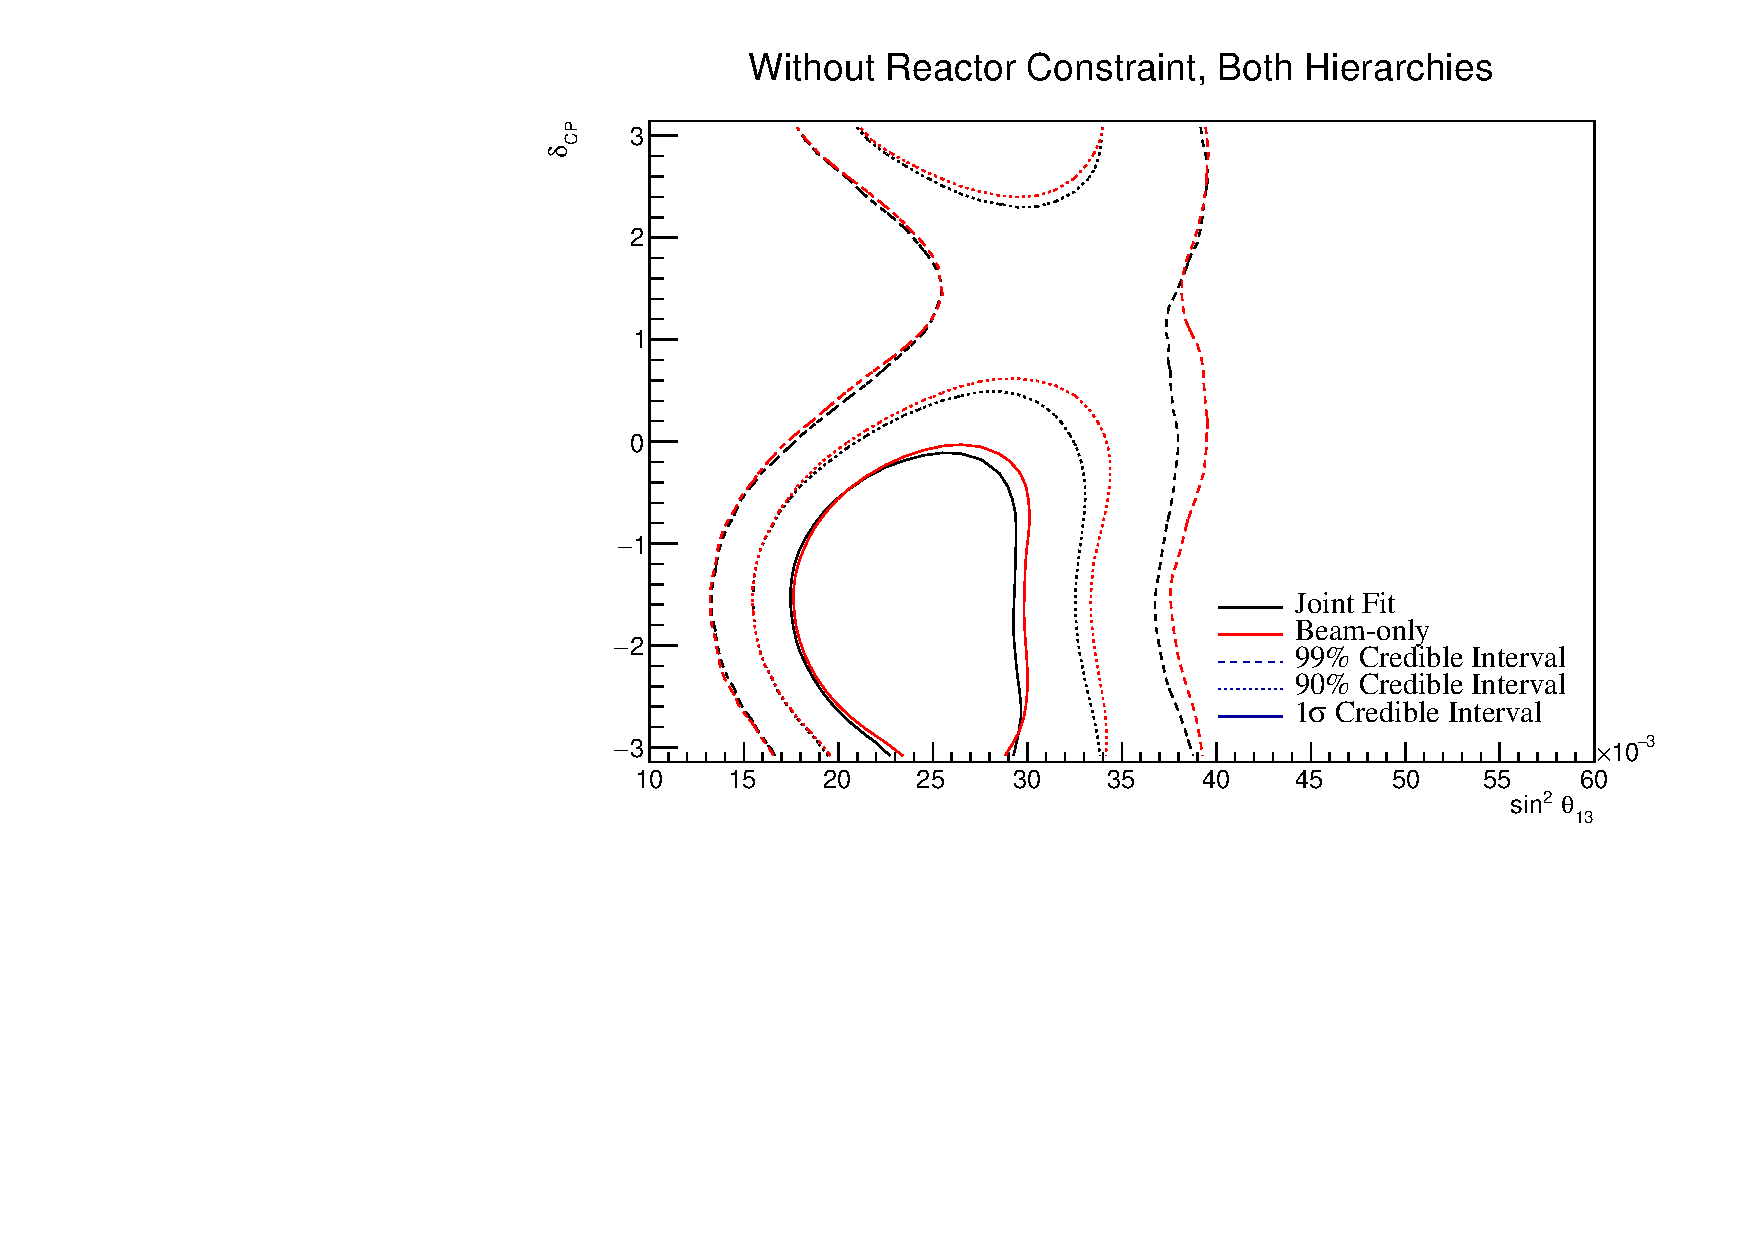
\includegraphics[width=\textwidth, trim={0mm 0mm 0mm 0mm}, clip,page=1]{Figures/OA/JointFit_OA2020_Comp/ContourComparison_2D_th13_dcp_BH_0_woRC_UnSmeared_CredibleInterval.pdf}
  \end{subfigure}
  \caption{The two-dimensional posterior probability density distribution in \quickmath{\delta_{CP}\text{\textendash}\sin^{2}(\theta_{13})} compared between the joint beam-atmospheric fit (Black) and the latest T2K sensitivities (Red) \cite{Dunne2020-uf, t2k_tn_393}. The reactor constraint is not applied in either fit. The distributions are marginalised over both hierarchies. The marker represents the known value of \quickmath{\delta_{CP}\text{\textendash}\sin^{2}(\theta_{13})}.}
  \label{fig:OscillationAnalysis_JointFit_OA2020_DCPTH13}
\end{figure}

\begin{figure}[h]
  \begin{subfigure}[t]{0.98\textwidth}
    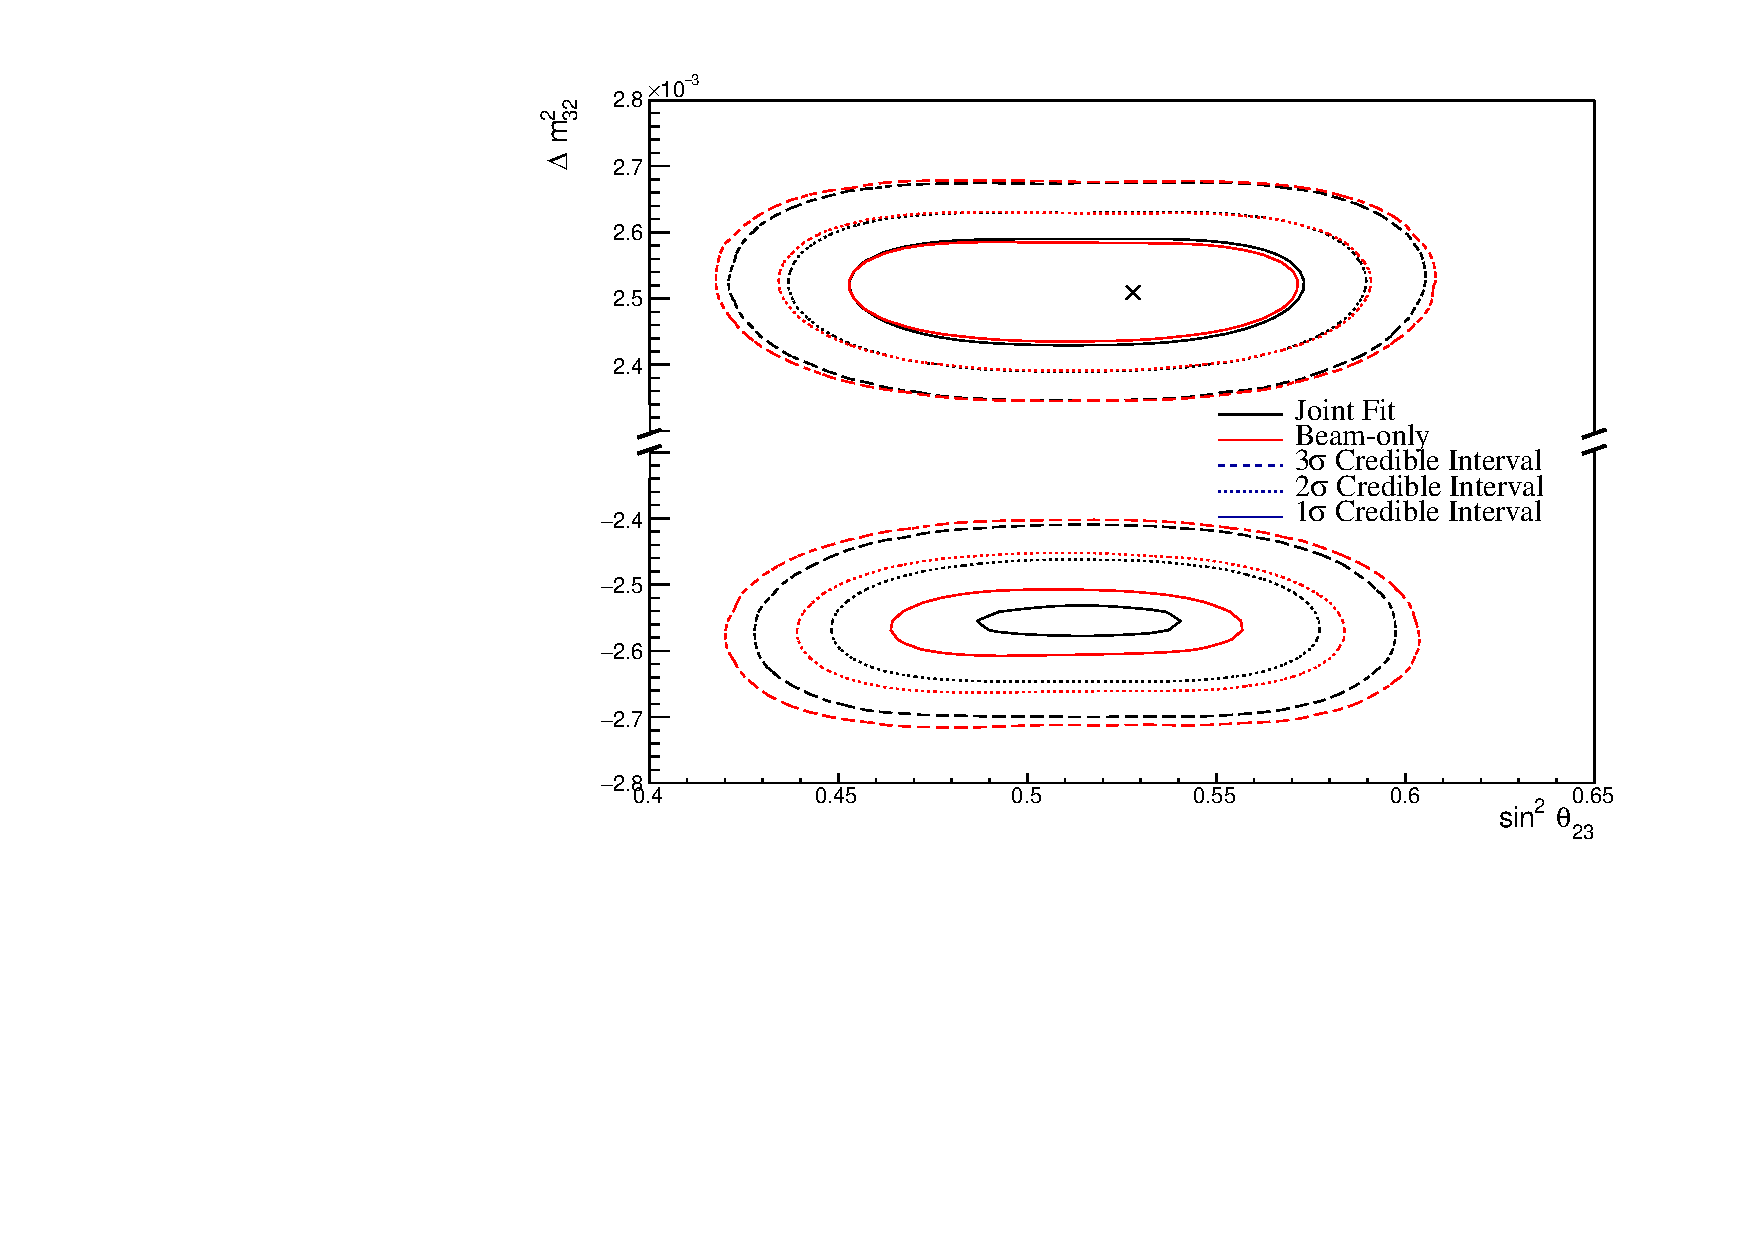
\includegraphics[width=\textwidth, trim={0mm 0mm 0mm 0mm}, clip,page=1]{Figures/OA/JointFit_OA2020_Comp/ContourComparison_2D_th23_dm32_BH_1_woRC_UnSmeared_CredibleInterval.pdf}
  \end{subfigure}
  \caption{The two-dimensional posterior probability density distribution in \quickmath{\Delta m^{2}_{32}\text{\textendash}\sin^{2}(\theta_{23})} compared between the joint beam-atmospheric fit (Black) and the latest T2K sensitivities (Red) \cite{Dunne2020-uf, t2k_tn_393}. The reactor constraint is not applied in either fit. The marker represents the known value of \quickmath{\Delta m^{2}_{32}\text{\textendash}\sin^{2}(\theta_{23})}.}
  \label{fig:OscillationAnalysis_JointFit_OA2020_DM32TH23}
\end{figure}

\begin{figure}[h]
  \begin{subfigure}[t]{0.98\textwidth}
    \includegraphics[width=\textwidth, trim={0mm 0mm 0mm 0mm}, clip,page=1]{Figures/OA/JointFit_OA2020_Comp/ContourComparison_2D_dcp_dm32_BH_1_woRC_UnSmeared_CredibleInterval.pdf}
  \end{subfigure}
  \caption{The two-dimensional posterior probability density distribution in \quickmath{\Delta m^{2}_{32}\text{\textendash}\Delta_{CP}} compared between the joint beam-atmospheric fit (Black) and the latest T2K sensitivities (Red) \cite{Dunne2020-uf, t2k_tn_393}. The reactor constraint is not applied in either fit. The marker represents the known value of \quickmath{\Delta m^{2}_{32}\text{\textendash}\Delta_{CP}}.}
  \label{fig:OscillationAnalysis_JointFit_OA2020_DM32DCP}
\end{figure}

The comparison in sensitivity to \quickmath{\delta_{CP}\text{\textendash}\Delta m^{2}_{32}} is illustrated in \autoref{fig:OscillationAnalysis_JointFit_OA2020_DM32DCP}. The contours from the joint beam-atmospheric fit are much smaller in the IH region as compared to the beam-only analysis. This culminates in a region around \quickmath{\delta_{CP} \sim \pi/2} in the H region which is excluded at \quickmath{3\sigma}. This behaviour is not present within the beam-only analysis. Consistent with the previous observations, the area contained within the IH credible intervals is significantly reduced in comparison to the beam-only analysis.

The sensitivity to \quickmath{\Delta m^{2}_{32}}, as a function of \quickmath{\sin^{2}(\theta_{13})}, is presented in \autoref{fig:OscillationAnalysis_JointFit_OA2020_DM32TH13}. Similar to previous observations, the \quickmath{\Delta m^{2}_{32}} contours within IH region of the joint fit are much smaller than the beam-only analysis. Notably, the joint fit IH \quickmath{1\sigma} credible intervals exclude the region around the reactor constraint. This suggests that the application of the reactor constraint would further increase the preference for NH in the joint fit compared to its effect on the beam-only analysis.

The beam-only and joint beam-atmospheric fits have a slightly different contour shape between the \quickmath{\sin^{2}(\theta_{13})} and \quickmath{\sin^{2}(\theta_{23})} parameters, as illustrated by \autoref{fig:OscillationAnalysis_JointFit_OA2020_TH13TH23}. The joint analysis disfavours the wrong octant hypothesis more strongly in the region of high \quickmath{\sin^{2}(\theta_{13})}. This change in correlation means that the application of the reactor constraint could affect the two analyeses differently.
%suggests that the application of the reactor constraint will favour the UO more strongly in the joint analysis compared to the beam-only analysis.

\begin{figure}[h]
  \begin{subfigure}[t]{0.98\textwidth}
    \includegraphics[width=\textwidth, trim={0mm 0mm 0mm 0mm}, clip,page=1]{Figures/OA/JointFit_OA2020_Comp/ContourComparison_2D_th13_dm32_BH_0_woRC_UnSmeared_CredibleInterval.pdf}
  \end{subfigure}
  \caption{The two-dimensional posterior probability density distribution in \quickmath{\Delta m^{2}_{32}\text{\textendash}\sin^{2}(\theta_{23})} compared between the joint beam-atmospheric fit (Black) and the latest T2K sensitivities (Red) \cite{Dunne2020-uf, t2k_tn_393}. The reactor constraint is not applied in either fit. The marker represents the known value of \quickmath{\Delta m^{2}_{32}\text{\textendash}\sin^{2}(\theta_{23})}.}
  \label{fig:OscillationAnalysis_JointFit_OA2020_DM32TH13}
\end{figure}

\begin{figure}[h]
  \begin{subfigure}[t]{0.98\textwidth}
    \includegraphics[width=\textwidth, trim={0mm 0mm 0mm 0mm}, clip,page=1]{Figures/OA/JointFit_OA2020_Comp/ContourComparison_2D_th13_th23_BH_1_woRC_UnSmeared_CredibleInterval.pdf}
  \end{subfigure}
  \caption{The two-dimensional posterior probability density distribution in \quickmath{\sin^{2}(\theta_{23})\text{\textendash}\sin^{2}(\theta_{13})} compared between the joint beam-atmospheric fit (Black) and the latest T2K sensitivities (Red) \cite{Dunne2020-uf, t2k_tn_393}. The reactor constraint is not applied in either fit. The distributions are marginalised over both hierarchies. The marker represents the known value of \quickmath{\sin^{2}(\theta_{23})\text{\textendash}\sin^{2}(\theta_{13})}.}
  \label{fig:OscillationAnalysis_JointFit_OA2020_TH13TH23}
\end{figure}

\clearpage
\subsection{Comparison to Latest T2K Sensitivities with Reactor Constraint}
\label{sec:OscillationAnalysis_JointFit_OA2020_wRC}
%The comparison between the beam-only and joint beam-atmospheric fits are compared in \autoref{sec:OscillationAnalysis_JointFit_OA2020}. Those comparisons were made with the reactor constraint not applied to either of the fits.
This section illustrates the comparison between the joint beam-atmospheric and beam-only fits when the reactor constraint is applied. As shown in \autoref{fig:OscillationAnalysis_JointFit_OA2020_DM32TH13}, the application of the reactor constraint is expected to significantly increase the joint fit's preference for the NH hypothesis, compared to the beam-only analysis. \autoref{fig:OscillationAnalysis_JointFit_OA2020_wRC_TH23DM32} illustrates the sensitivities of the two fits to the disappearance parameters (\quickmath{\sin^{2}(\theta_{23})\text{\textendash}\Delta m^{2}_{32}}). This plot further illustrates the benefit of the joint beam-atmospheric analysis. The \quickmath{1\sigma} credible interval in the IH region is entirely removed in the joint analysis but not for the beam-only analysis.

\begin{figure}[h]
  \begin{subfigure}[t]{0.98\textwidth}
    \includegraphics[width=\textwidth, trim={0mm 0mm 0mm 0mm}, clip,page=1]{Figures/OA/JointFit_OA2020_wRC_Comp/ContourComparison_2D_th23_dm32_BH_1_wRC_UnSmeared_CredibleInterval.pdf}
  \end{subfigure}
  \caption{The two-dimensional posterior probability density distribution in \quickmath{\Delta m^{2}_{32}\text{\textendash}\sin^{2}(\theta_{23})} compared between the joint beam-atmospheric fit (Black) and the latest T2K sensitivities (Red) \cite{Dunne2020-uf, t2k_tn_393}. The reactor constraint is applied in both fits. The marker represents the known value of \quickmath{\Delta m^{2}_{32}\text{\textendash}\sin^{2}(\theta_{23})}.}
  \label{fig:OscillationAnalysis_JointFit_OA2020_wRC_TH23DM32}
\end{figure}

The credible intervals of the joint fit are also tighter in the \quickmath{\sin^{2}(\theta_{23})} dimension than the beam-only analysis in both mass hierarchy regions. This shows that beyond the ability of the joint fit to prefer the NH more strongly than the beam-only analysis, the precision to which it can measure \quickmath{\sin^{2}(\theta_{23})} is also improved. The Bayes factor for NH preference is calculated as \quickmath{B(\text{NH}/\text{IH}) = 6.47} and \quickmath{B(\text{NH}/\text{IH}) = 3.09} for the joint beam-atmospheric and beam-only analysis, respectively. This important conclusion illustrates that the joint beam-atmospheric analysis can provide a substantial preference for the correct hypothesis (NH) whilst the beam-only analysis can not.

The Bayes factors for UO preference which are \quickmath{B(\text{UO}/\text{LO}) = 2.86} and \quickmath{B(\text{UO}/\text{LO}) = 2.47} for the joint beam-atmospheric and beam-only analysis, respectively. Both of these represent a mild preference for the correct octant (UO) but a stronger preference is observed in the joint analysis.

The sensitivity of the beam-only and joint beam-atmospheric analyses, to the appearance parameters (\quickmath{\delta_{CP}\text{\textendash}\sin^{2}(\theta_{13})}), are compared in \autoref{fig:OscillationAnalysis_JointFit_OA2020_wRC_TH13DCP}. These results are marginalised over both hierarchies. For this particular set of known oscillation parameters (AsimovA defined in \autoref{tab:Theory_ParameterSets}), the beam-only analysis dominates the sensitivity. The joint fit does slightly increase the sensitivity to \quickmath{\delta_{CP}} but it does not change any conclusions that would be made. As expected, the prior knowledge dominates any sensitivity either fit would have on \quickmath{\sin^{2}(\theta_{13})}.

\begin{figure}[h]
  \begin{subfigure}[t]{0.98\textwidth}
    \includegraphics[width=\textwidth, trim={0mm 0mm 0mm 0mm}, clip,page=1]{Figures/OA/JointFit_OA2020_wRC_Comp/ContourComparison_2D_th13_dcp_BH_1_wRC_UnSmeared_CredibleInterval.pdf}
  \end{subfigure}
  \caption{The two-dimensional posterior probability density distribution in \quickmath{\delta_{CP}\text{\textendash}\sin^{2}(\theta_{13})} compared between the joint beam-atmospheric fit (Black) and the latest T2K sensitivities (Red) \cite{Dunne2020-uf, t2k_tn_393}. The reactor constraint is applied in both fits. The distributions are marginalised over both hierarchies. The marker represents the known value of \quickmath{\delta_{CP}\text{\textendash}\sin^{2}(\theta_{13})}.}
  \label{fig:OscillationAnalysis_JointFit_OA2020_wRC_TH13DCP}
\end{figure}

\clearpage
\subsection{Alternate Asimov Parameter Set}
\label{sec:OscillationAnalysis_AsimovB}

\autoref{fig:OscillationAnalysis_AsimovEval_DCP} and \autoref{fig:OscillationAnalysis_AsimovEval_TH23} show that the choice of the parameter set at which the Asimov data is made can affect the conclusion. `AsimovA' oscillation parameters are defined at a region of \quickmath{\delta_{CP}} which is preferred by the T2K experiment. This explains why the addition of the atmospheric samples does not significantly increase the sensitivity to \quickmath{\delta_{CP}}, as illustrated in \autoref{sec:OscillationAnalysis_JointFit_OA2020} and \autoref{sec:OscillationAnalysis_JointFit_OA2020_wRC}. This section presents the sensitivities when `AsimovB' oscillation parameters, as defined in \autoref{tab:Theory_ParameterSets}, are assumed (alongside the post-BANFF tune) when building the Asimov data.

\begin{figure}[h]
  \begin{subfigure}[t]{0.98\textwidth}
    \includegraphics[width=\textwidth, trim={0mm 0mm 0mm 0mm}, clip,page=1]{Figures/OA/JointFit_OA2020_Comp_AsimovB/ContourComparison_1D_dcp_BH_2_woRC_UnSmeared_CredibleInterval.pdf}
  \end{subfigure}
  \caption{The one-dimensional posterior probability density distribution in \quickmath{\delta_{CP}} compared between the joint beam-atmospheric fit (Black) and the latest T2K sensitivities (Red) \cite{Dunne2020-uf, t2k_tn_393}. The reactor constraint is not applied in either fit. The distributions are marginalised over both hierarchies. The vertical dashed line represents the known value of \quickmath{\delta_{CP}}.}
  \label{fig:OscillationAnalysis_JointFit_AsimovB_DCP}
\end{figure}

The sensitivity to \quickmath{\delta_{CP}} for the joint beam-atmospheric fit is presented in \autoref{fig:OscillationAnalysis_JointFit_AsimovB_DCP}. The results are compared to those from the beam-only analysis in \cite{Dunne2020-uf, t2k_tn_393}. The reactor constraint is not applied in either of the fits. The shape of the posterior distribution from the joint analysis is more peaked at the known oscillation parameter value compared to the beam-only analysis, which has approximately the same posterior probability density at \quickmath{\delta_{CP} = 0} and \quickmath{\delta_{CP} = \pm\pi}. This shows the ability of the joint analysis to better determine the correct phase of \quickmath{\delta_{CP}} if the true value were CP-conserving. The \quickmath{1\sigma} credible intervals and the position of the highest posterior probability density are given in \autoref{tab:OscillationAnalysis_JointFit_AsimovB_CredIntervals}. The highest posterior density for the joint beam-atmospheric analysis is \quickmath{\delta_{CP} = -0.06 \pm 0.06} which is consistent with the known value.

\begin{table}[ht!]
  \centering
  \begingroup
  \renewcommand{\arraystretch}{1.5}
  \begin{tabular}{c|c|c}
    Parameter               & Interval & HPD \\ \hline
    \quickmath{\delta_{CP}, \text{ (BH)}} & \quickmath{\left[ -\pi, -2.51 \right], \left[ -1.51, 1.13 \right]} & \quickmath{-0.06 \pm 0.06} \\
    \quickmath{\delta_{CP}, \text{ (NH)}} & \quickmath{\left[ -1.13, 1.63 \right]} & \quickmath{0.06 \pm 0.06} \\
    \quickmath{\delta_{CP}, \text{ (IH)}} & \quickmath{\left[ -3.02, -1.88 \right], \left[ -1.76, 0.13 \right]} & \quickmath{-0.44 \pm 0.06} \\ \hline
    \quickmath{\Delta m^{2}_{32} \text{ (BH) } [\times 10^{-3} \text{eV}^{2}]} & \quickmath{\left[ -2.60, -2.52 \right], \left[ 2.46, 2.56 \right]} & \quickmath{2.51 \pm 0.01} \\
    \quickmath{\Delta m^{2}_{32} \text{ (NH) } [\times 10^{-3} \text{eV}^{2}]}& \quickmath{\left[ 2.47, 2.56 \right]} & \quickmath{2.52 \pm 0.01} \\
    \quickmath{\Delta m^{2}_{32} \text{ (IH) } [\times 10^{-3} \text{eV}^{2}]} & \quickmath{\left[ -2.61, -2.52 \right]} & \quickmath{-2.57 \pm 0.01} \\ \hline
    \quickmath{\sin^{2}(\theta_{23}) \text{ (BH) }} & \quickmath{\left[ 0.430, 0.480 \right], \left[ 0.545, 0.585 \right]} & \quickmath{0.453 \pm 0.003} \\
    \quickmath{\sin^{2}(\theta_{23}) \text{ (NH) }} & \quickmath{\left[ 0.430, 0.485 \right], \left[ 0.550, 0.580 \right]} & \quickmath{0.453 \pm 0.003} \\
    \quickmath{\sin^{2}(\theta_{23}) \text{ (IH) }} & \quickmath{\left[ 0.435, 0.480 \right], \left[ 0.540, 0.585 \right]} & \quickmath{0.568 \pm 0.003} \\ \hline \hline
  \end{tabular}
  \caption{The position of the highest posterior probability density (HPD) and width of the \quickmath{1\sigma} credible interval for the joint beam-atmospheric fit. The reactor constraint is not applied. The values are presented by which hierarchy hypothesis is assumed: marginalised over both hierarchies (BH), normal hierarchy only (NH) and inverted hierarchy only (IH).}
  \label{tab:OscillationAnalysis_JointFit_AsimovB_CredIntervals}
  \endgroup
\end{table}

Naively, if just the \quickmath{1\sigma} credible interval were considered without observing the shape of the distribution, it would appear that the joint analysis would have a worse sensitivity to \quickmath{\delta_{CP}} due to the larger interval around \quickmath{\delta_{CP} = 0}. The \quickmath{1\sigma} credible interval for the beam-only analysis is given as the range \quickmath{\delta_{CP} = [-\pi, -1.88], [-1.13, 0.63]} and \quickmath{[2.64, \pi]} which contains \quickmath{56\%} of all values of \quickmath{\delta_{CP}}. Whereas, the joint beam-atmospheric analysis contains \quickmath{52\%} of all \quickmath{\delta_{CP}} values within the \quickmath{1\sigma} credible interval. Therefore, if the area within the \quickmath{1\sigma} credible interval were to be compared between the two fits, the joint analysis would be shown to have better precision.

This apparent contradiction stems from the methodology in which the credible interval is calculated. The technique used in this analysis (documented in \autoref{sec:MarkovChainMonteCarlo_ParameterEstimation}) fills the credible interval by selecting bins in order of probability density until \quickmath{68\%} of the posterior density is contained. If instead, the credible interval were calculated by expanding around the highest posterior probability, the benefits of the joint fit would be more obvious. In the case where the shape of the posterior was uni-modal, these two techniques would be equivalent to statistical fluctuations.

\begin{figure}[h]
  \begin{subfigure}[t]{0.98\textwidth}
    \includegraphics[width=\textwidth, trim={0mm 0mm 0mm 0mm}, clip,page=1]{Figures/OA/JointFit_OA2020_Comp_AsimovB/ContourComparison_1D_th23_BH_2_woRC_UnSmeared_CredibleInterval.pdf}
  \end{subfigure}
  \caption{The one-dimensional posterior probability density distribution in \quickmath{\sin^{2}(\theta_{23})} compared between the joint beam-atmospheric fit (Black) and the latest T2K sensitivities (Red) \cite{Dunne2020-uf, t2k_tn_393}. The reactor constraint is not applied in either fit. The distributions are marginalised over both hierarchies. The vertical dashed line represents the known value of \quickmath{\sin^{2}(\theta_{23})}.}
  \label{fig:OscillationAnalysis_JointFit_AsimovB_TH23}
\end{figure}

The sensitivity of the joint beam-atmospheric fit to \quickmath{\sin^{2}(\theta_{23})} is presented in \autoref{fig:OscillationAnalysis_JointFit_AsimovB_TH23}. The sensitivity is compared to that of the beam-only analysis in \cite{Dunne2020-uf, t2k_tn_393}. The reactor constraint is not applied in either of the fits being compared. The joint beam-atmospheric fit has a much larger probability density in the region surrounding the known oscillation parameter, \quickmath{\sin^{2}(\theta_{23}) = 0.45}. This shows the better octant determination of the joint analysis compared to the beam-only fit. The ratio of the posterior density at the peak of the lower octant to the peak of the upper octant from the joint fit is \quickmath{1.43} compared to \quickmath{1.09} from the beam-only analysis. The area contained within the \quickmath{1\sigma} credible interval for the joint analysis is \quickmath{\sin^{2}(\theta_{23}) = [0.430,0.480]} and \quickmath{\sin^{2}(\theta_{23}) = [0.545,0.585]}, whereas the beam-only analysis includes \quickmath{\sin^{2}(\theta_{23}) = [0.435,0.485]} and \quickmath{\sin^{2}(\theta_{23}) = [0.540,0.585]}. This corresponds to a \quickmath{\sim 5\%} (binning dependent) increase in preecision from the joint analysis.
%This shows further support for the joint analysis in correctly selecting the lower octant, which is the correct hypothesis given the known oscillation parameters.

\begin{table}[ht!]
  \centering
  \begingroup
  \renewcommand{\arraystretch}{1.5}
  \begin{tabular}{c|cc|c}
                                                        & LO \quickmath{\left(\sin^{2}\theta_{23} < 0.5 \right)} & UO \quickmath{\left( \sin^{2}\theta_{23} > 0.5 \right)} & Sum  \\ \hline
    NH \quickmath{\left( \Delta m^{2}_{32} > 0 \right)} &                                                   0.35 &                                                    0.24 & 0.59 \\
    IH \quickmath{\left( \Delta m^{2}_{32} < 0 \right)} &                                                   0.19 &                                                    0.22 & 0.41 \\ \hline
    Sum                                                 &                                                   0.54 &                                                    0.46 & 1.00 \\       
  \end{tabular}
  \caption{The distribution of steps in a joint beam-atmospheric fit, presented as the fraction of steps in the upper (UO) and lower (LO) octants and the normal (NH) and inverted (IH) hierarchies. The reactor constraint is not applied. The Bayes factors are calculated as \quickmath{B(\text{NH}/\text{IH}) = 1.43} and \quickmath{B(\text{LO}/\text{UO}) = 1.19}.}
  \label{tab:OscillationAnalysis_JointFit_BayesFactors_AsimovB}
  \endgroup
\end{table}

The distribution of steps, split by hierarchy and octant hypothesis, is presented in \autoref{tab:OscillationAnalysis_JointFit_BayesFactors_AsimovB}. The Bayes factor for hierarchy and octant determination are \quickmath{B(\text{NH}/\text{IH}) = 1.43} and \quickmath{B(\text{LO}/\text{UO}) = 1.19}, respectively.
%The octant Bayes factor is now presented as \quickmath{\text{LO}/\text{UO}} as the known oscillation parameter is contained within the lower octant.
These values compare to \quickmath{B(\text{NH}/\text{IH}) = 1.08} and \quickmath{B(\text{LO}/\text{UO}) = 0.91} from the beam-only analysis. This evidences the joint analysis's ability to select the correct octant and hierarchy hypothesis. Comparisons to the AsimovA Bayes factors presented in \autoref{tab:OscillationAnalysis_JointFit_BayesFactors} show how the preferences for the correct octant and hierarchy depend on the true value of \quickmath{\delta_{CP}} and \quickmath{\sin^{2}(\theta_{23})}.

\begin{figure}[h]
  \begin{subfigure}[t]{0.98\textwidth}
    \includegraphics[width=\textwidth, trim={0mm 0mm 0mm 0mm}, clip,page=1]{Figures/OA/JointFit_OA2020_Comp_AsimovB/ContourComparison_1D_dm32_BH_2_woRC_UnSmeared_CredibleInterval.pdf}
  \end{subfigure}
  \caption{The one-dimensional posterior probability density distribution in \quickmath{\Delta m^{2}_{32}} compared between the joint beam-atmospheric fit (Black) and the latest T2K sensitivities (Red) \cite{Dunne2020-uf, t2k_tn_393}. The reactor constraint is not applied in either fit. The vertical dashed line represents the known value of \quickmath{\Delta m^{2}_{32}}.}
  \label{fig:OscillationAnalysis_JointFit_AsimovB_DELM23}
\end{figure}

The sensitivity of the beam-only and joint beam-atmospheric analysis to \quickmath{\Delta m^{2}_{32}} is given in \autoref{fig:OscillationAnalysis_JointFit_AsimovB_DELM23}. The joint analysis has a stronger preference for the correct hierarchy (NH) which is shown by the higher Bayes factor compared to the beam-only analysis. This is further evidenced by the width of the \quickmath{90\%} credible interval in the IH region being tighter in the joint analysis compared to the beam-only analysis.

\clearpage
\subsection{Effect of Systematics}
\label{sec:EffectOfSystematics}

The effect of systematics on each sample used in this analysis is calculated using the posterior predictive method documented in \autoref{sec:MarkovChainMonteCarlo_Predictives}. The distribution of each sample's spectrum has been generated by sampling \quickmath{2000} steps from the posterior distribution of the joint beam-atmospheric fit. This technique reweights the Monte Carlo prediction using the systematic values given by a particular step, stores the sample spectra, and repeats for the desired number of steps. The oscillation parameters are always fixed at Asimov A values to only study the effect of systematic parameters.

\autoref{fig:OscillationAnalysis_PosteriorPredictive_SG_elike0dcy} illustrates the distribution for the \texttt{SubGeV-elike-0dcy} atmospheric sample. The fit being sampled is detailed in \autoref{sec:OscillationAnalysis_JointFit}. The distribution closely resembles the Asimov data spectrum. This would be expected from an Asimov fit where the Monte Carlo is fit to itself but gives more credibility to the results of the fit.

\begin{figure}[h]
  \begin{subfigure}[t]{0.98\textwidth}
    \includegraphics[width=\textwidth, trim={0mm 0mm 0mm 0mm}, clip,page=1]{Figures/OA/Predictive_AllSyst.pdf}
  \end{subfigure}
  \caption{Result of the posterior predictive method for the \texttt{SubGeV\_elike\_0dcy} sample after sampling \quickmath{2000} steps from the joint beam-atmospheric chain detailed in \autoref{sec:OscillationAnalysis_JointFit} (Coloured histogram). The mean and uncertainty is presented for each bin. The Asimov data prediction (denoted `Post BANFF Spectra', Red) assumes the post-BANFF tune and Asimov A oscillation parameters.}
  \label{fig:OscillationAnalysis_PosteriorPredictive_SG_elike0dcy}
\end{figure}

The total event rate for each sample from each of the sampled steps is calculated and the fractional uncertainty, \quickmath{\Delta N_{i}/N_{i}} where \quickmath{N_{i}} is the event rate of the \quickmath{i^{th}} sample, is calculated. These values are presented in \autoref{tab:OscillationAnalysis_PosteriorPredEventRateUncertainty}. In general, the impact of the systematics has a \quickmath{\sim 3\%} uncertainty on the event rate of atmospheric samples, where CC\quickmath{1\pi}-targeting samples have slightly larger uncertainties than the CCQE-like samples.
%The low energy atmospheric samples have similar uncertainty as the beam samples with uncertainties \quickmath{O(3\%)}.
%The CC\quickmath{1\pi}-like targeting samples have a larger uncertainty due to the additional ad-hoc systematics invoked within this analysis.
The fractional uncertainties on the beam samples are compared to those from the beam-only analysis presented in \cite{Dunne2020-uf, t2k_tn_393}. The uncertainties on the one-ring muon samples are mostly unchanged, whereas the uncertainties on the one-ring electron samples are different. As discussed in \autoref{sec:OscillationAnalysis_LLHScans}, the atmospheric samples should be able to add constraints on the NC background events present in the \texttt{FHC1Re} and \texttt{RHC1Re} samples. The uncertainty reduction seen in those samples is due to those additional constraints. The reason why the \texttt{FHC1Re1de} has a higher uncertainty in this analysis is due to the addition of the ad-hoc systematic introduced for CC\quickmath{1\pi} interactions (see \autoref{sec:SelsAndSysts_Systs_Interaction}).

\begin{table}[ht!]
    \centering
    \begin{tabular}{|l|c|c|}
      \hline
      & \multicolumn{2}{|c|}{Percentage Uncertainty (\%)} \\
      \hline
      Sample & Joint Analysis & Beam-only Analysis \\
      \hline
      \texttt{SubGeV-elike-0dcy} & 2.53 & - \\
      \texttt{SubGeV-elike-1dcy} & 3.28 & - \\
      \texttt{SubGeV-mulike-0dcy} & 2.62 & - \\
      \texttt{SubGeV-mulike-1dcy} & 2.23 & - \\
      \texttt{SubGeV-mulike-2dcy} & 3.96 & - \\
      \texttt{SubGeV-pi0like} & 2.84 & - \\
      \texttt{MultiGeV-elike-nue} & 5.14 & - \\
      \texttt{MultiGeV-elike-nuebar} & 2.79 & - \\
      \texttt{MultiGeV-mulike} & 2.99 & - \\
      \texttt{MultiRing-elike-nue} & 2.94 & - \\
      \texttt{MultiRing-elike-nuebar} & 2.83 & - \\
      \texttt{MultiRing-mulike} & 2.89 & - \\
      \texttt{MultiRingOther-1} & 2.70 & - \\
      \texttt{PCStop} & 3.22 & - \\
      \texttt{PCThru} & 2.99 & - \\
      \texttt{UpStop-mu} & 2.95 & - \\
      \texttt{UpThruNonShower-mu} & 2.70 & - \\
      \texttt{UpThruShower-mu} & 3.19 & - \\
      \texttt{FHC1Rmu} & 2.49 & 2.33 \\
      \texttt{RHC1Rmu} & 2.89 & 2.93 \\
      \texttt{FHC1Re} & 4.12 & 4.57 \\
      \texttt{RHC1Re} & 5.15 & 5.65 \\
      \texttt{FHC1Re1de} & 13.38 & 11.51 \\
      \hline
      \hline
    \end{tabular}
    \caption{The percentage uncertainty, \quickmath{\Delta N/N}, as calculated from sampling \quickmath{2000} throws from a joint beam-atmospheric chain. The same values for the beam samples are provided from the beam-only analysis \cite{Dunne2020-uf, t2k_tn_393}. These uncertainties consider all systematic parameters to be sampled from the fit whilst the oscillation parameters are fixed at the Asimov A oscillation set.}
    \label{tab:OscillationAnalysis_PosteriorPredEventRateUncertainty}
\end{table}

Beyond the impact of the uncertainty on each sample's event rate, the post-fit constraint on each systematic parameter should be checked. \autoref{fig:OscillationAnalysis_ParameterConstraints} illustrates the central value and uncertainty on a select group of interaction systematics, for both the joint beam-atmospheric (from \autoref{sec:OscillationAnalysis_JointFit}) and the beam-only analysis. From the discussion in \autoref{sec:OscillationAnalysis_LLHScans}, the uncertainty on systematics which are strongly constrained by the near detector should not significantly change when adding the atmospheric analysis. This behaviour is evidenced by the fact that the ratio of constraints between the two fits are very similar (within a few \quickmath{\%}) for almost all systematics. The only systematic which is more constrained in the joint beam-atmospheric analysis is the \quickmath{NC Other SK} normalisation parameter, which has a \quickmath{O(10\%)} tighter constraint. As expected, the atmospheric samples have been able to constrain this systematic which leads to the reduction in uncertainty for the beam electron-like samples.

\begin{figure}[h]
  \begin{subfigure}[t]{0.98\textwidth}
    \includegraphics[width=\textwidth, trim={0mm 0mm 0mm 0mm}, clip,page=1]{Figures/OA/FitComparison.pdf}
  \end{subfigure}
  \begin{subfigure}[t]{0.98\textwidth}
    \includegraphics[width=\textwidth, trim={0mm 0mm 0mm 0mm}, clip,page=4]{Figures/OA/FitComparison.pdf}
  \end{subfigure}
  \caption{Central values and \quickmath{1\sigma} uncertainties for a select group of interaction systematics. The constraints from the prior uncertainty (Black), joint atmospheric-beam fit given in \autoref{sec:OscillationAnalysis_JointFit} (Red) and beam-only analysis \cite{Dunne2020-uf, t2k_tn_393} (Blue) are presented. The top part of each plot presents the parameter variation and the bottom part represents the ratio of the uncertainty between the joint beam-atmospheric and beam-only fits, where a value below \quickmath{1.0} means the joint fit has a tighter constraint than the beam-only analysis. }
  \label{fig:OscillationAnalysis_ParameterConstraints}
\end{figure}

\clearpage
\subsection{Alternative Detector Model Concept}
\label{sec:AlternativeDetectorModel}
\finish{Complete this section}

As a plausible extension to the analysis already presented, this section considers the joint beam-atmospheric fit results when the correlated detector model documented in \autoref{sec:SelsAndSysts_Systs_Correlated} is used instead of the inputs provided by the two experiments. The results shown here should be considered preliminary as the results need further investigation to ensure their reliability. This technique fits the detector systematics simultaneously with the sample spectra so the definition of the likelihood, given in \autoref{sec:OscillationAnalysis_LLHCalc}, needs to be modified. Following the method outlined in \finish{Xiaoyue's thesis}, an additional term needs to be added to the likelihood. This additional term is,

\begin{equation}
  \label{eqn:Likelihood:Likelihood_CorrelatedDetectorModel}
  \begin{split}
    & \frac{1}{2} \sum^{SG Samples}_s \sum^{E_{k} bins}_{k} \left(\rho(R_s | E_k, \vec{\theta}) \rho(P^{e/\mu}_s | E_k, \vec{\theta}) \rho(P^{e/\pi^0}_s | E_k, \vec{\theta}) \rho(P^{\mu/\pi^+}_s | E_k, \vec{\theta}) \right).
  \end{split}
\end{equation}

This fits the ring counting $R_s$, electron-muon $P^{e/\mu}$, electron-neutral pion $P^{e/\pi^0}$ and muon-charged pion $P^{\mu/\pi^+}$ particle identification distribution parameters, in bins of visible energy $E_k$, of the SubGeV atmospheric and beam samples (SG). In the situation where infinite Monte Carlo statistics were generated, a many-dimensional (the reconstructed lepton momentum and direction and the four particle identification parameters in the case of an atmospheric sample) spectra could be determined. However, this is not the case so the standard spectra (reconstructed lepton momentum and direction) is fit along with four one-dimensional distribution of each parameter identification parameter. Therefore, shape-likelihoods are used for each particle identification parameter,

\begin{equation}
\rho(X | E_k, \vec{\theta}) = \sum^{j}_{i = 0} \left[ N_i^d \times \log \left( \frac{N_i^p (\vec{\theta})}{\sum^{X}_{i = 0}N_i^p (\vec{\theta})} \right) \right].
\end{equation}

Where \quickmath{X} refers to a particle identification parameter, $N_{i}^{p(d)}$ refers to the \quickmath{i^{th}} bin value from the predicted MC distribution (data distribution) and \quickmath{j} reprresents the total bin number of the \quickmath{X} distribution.

\clearpage
\section{Summary of Sensitivity Studies}
\label{sec:OA_Summary}

The sensitivities to each oscillation parameter from the joint beam-atmospheric and beam-only fits, which use the Asimov A oscillation parameter set, are summarised in \autoref{tab:OscillationAnalysis_MeasurementSummary}. As the posterior distribution to \quickmath{\delta_{CP}} is cyclical, only the position of the highest posterior density (HPD) is given. The uncertainty corresponds to the width of the bin in which the HPD is located. Furthermore, the \quickmath{\Delta m^{2}_{32}} reported values only consider the NH credible interval region as the full discussion can be found in the previous section.

\begin{table}[ht!]
  \centering
  \begingroup
  \renewcommand{\arraystretch}{1.5}
  \begin{tabular}{|l|c|c|c|c|}
    \hline
    Fit & \quickmath{\delta_{CP}} (HPD) & \quickmath{\Delta m^{2}_{32} [\times 10^{-3} \text{eV}^{2}]} & \quickmath{\sin^{2}(\theta_{23})} & \quickmath{\sin^{2}(\theta_{13}) [\times 10^{-2}]} \\
    \hline
    \hline
    Asimov A & \quickmath{-1.601} & \quickmath{2.509} & \quickmath{0.528} & \quickmath{2.19} \\
    \hline
    Beam & \quickmath{-1.45 \pm 0.06} & \quickmath{2.51^{+0.07}_{-0.06}} & \quickmath{0.501^{+0.044}_{-0.026}} & \quickmath{2.45^{+0.45}_{-0.35}} \\
    Beam w/RC & \quickmath{-1.57 \pm 0.06} & \quickmath{2.51^{+0.08}_{-0.06}} & \quickmath{0.533^{+0.022}_{-0.043}} & \quickmath{2.19^{+0.06}_{-0.07}} \\
    Joint & \quickmath{-1.57 \pm 0.06} & \quickmath{2.51^{+0.07}_{-0.06}} & \quickmath{0.518^{+0.027}_{-0.038}} & \quickmath{2.35^{+0.45}_{-0.35}} \\
    Joint w/RC & \quickmath{-1.57 \pm 0.06} & \quickmath{2.51^{+0.05}_{-0.06}} & \quickmath{0.528^{+0.027}_{-0.038}} & \quickmath{2.18^{+0.07}_{-0.06}} \\
    \hline
    \hline
%    Asimov B & \quickmath{0.} & \quickmath{2.509} & \quickmath{0.45} & \quickmath{2.19} \\
%    \hline
%    Beam & \quickmath{-0.19 \pm 0.06} & \quickmath{2.51^{+0.05}_{-0.05}} & \quickmath{0.453^{+0.018}_{-0.032}} & \quickmath{1.85^{+0.55}_{-0.35}} \\
%    Beam w/RC & \quickmath{-1.57 \pm 0.06} & \quickmath{2.57^{+0.}_{-0.11}} & \quickmath{0.453^{+0.027}_{-0.038}} & \quickmath{2.18^{+0.06}_{-0.07}} \\
%    Joint & \quickmath{-0.06 \pm 0.06} & \quickmath{2.51^{+0.05}_{-0.05}} & \quickmath{0.453^{+0.027}_{-0.023}} & \quickmath{1.95^{+0.45}_{-0.45}} \\
%    Joint w/RC & \quickmath{-0.06 \pm 0.06} & \quickmath{2.51^{+0.05}_{-0.05}} & \quickmath{0.453^{+0.037}_{-0.023}} & \quickmath{2.18^{+0.06}_{-0.07}} \\
%    \hline
%    \hline
  \end{tabular}
  \caption{A comparison of the sensitivity to each oscillation parameter of interest, from the beam-only \cite{Dunne2020-uf, t2k_tn_393} and joint atmospheric-beam fits discussed within this thesis. The results are illustrated both with and without the reactor constraint (RC). The best-fit values are taken from the highest posterior density (HPD) and the error comes from the width of the one-dimensional \quickmath{1\sigma} credible intervals. As the posterior distribution in \quickmath{\delta_{CP}} is cyclical, the highest posterior distribution is given instead.}
  \label{tab:OscillationAnalysis_MeasurementSummary}
  \endgroup
\end{table}

The Bayes factors from the beam-only and joint atmospheric-beam analyses are presented in \autoref{tab:OscillationAnalysis_BayesFactorSummary}. The strength of each preference, from Jeffrey's scale (\autoref{tab:MarkovChainMonteCarlo_JeffreysScale}), is also given.

\begin{table}[ht!]
  \centering
  \begingroup
  \renewcommand{\arraystretch}{1.5}
  \begin{tabular}{|l|c|c|c|c|}
    \hline
    Fit & \multicolumn{2}{|c|}{\quickmath{B(\text{NH}/\text{IH})}} & \multicolumn{2}{|c|}{\quickmath{B(\text{UO}/\text{LO})}} \\
    \cline{1-5}
    & Value & Strength & Value & Strength \\
    \hline
    \hline
    \multicolumn{5}{|c|}{Asimov A} \\
    \cline{1-5}
    Beam & \quickmath{1.91} & Weak & \quickmath{1.56} & Weak \\
    Beam w/RC & \quickmath{3.09} & Weak & \quickmath{2.47} & Weak \\
    Joint & \quickmath{3.67} & Substantial & \quickmath{1.74} & Weak \\
    Joint w/RC & \quickmath{6.47} & Substantial & \quickmath{2.64} & Weak \\
    \hline
    \hline
    \multicolumn{5}{|c|}{Asimov B} \\
    \cline{1-5}
    Beam & \quickmath{1.08} & Weak & \quickmath{0.91} & Weak \\
    Beam w/RC & \quickmath{0.98} & Weak & \quickmath{1.15} & Weak \\
    Joint & \quickmath{1.43} & Weak & \quickmath{1.19} & Weak \\
    Joint w/RC & \quickmath{1.36} & Weak & \quickmath{1.52} & Weak \\
    \hline
    \hline
  \end{tabular}
  \caption{A comparison of the Bayes factors for mass hierarchy and \quickmath{\sin^{2}(\theta_{23})} octant hypotheses, from the beam-only \cite{Dunne2020-uf, t2k_tn_393} and joint atmospheric-beam fits discussed within this thesis. The results are illustrated both with and without the reactor constraint (RC). The strength of the preference for the normal mass hierarchy and upper octants are provided by Jeffrey's scale \autoref{tab:OscillationAnalysis_BayesFactorSummary}.}
  \label{tab:OscillationAnalysis_BayesFactorSummary}
  \endgroup
\end{table}

To summarise this information, the joint fit prefers a tighter \quickmath{1\sigma} credible interval in \quickmath{\sin^{2}(\theta_{23})} along with a stronger Bayes factor for preferring the correct octant hypothesis. The increase in sensitivity to \quickmath{|\Delta m^{2}_{32}|} between the two fits is negligible but the joint analysis substantially prefers the correct mass hierarchy hypothesis. It does not require any external constraints on \quickmath{\sin^{2}(\theta_{13})} to make this statement. The joint analysis also produces a value of \quickmath{\sin^{2}(\theta_{13})} closer to the known value compared to the beam-only analysis. When the reactor constraint is applied, the preference for the correct hierarchy and octant (NH and UO) hypotheses increase but does not change the statement which would be made.

The fits from the Asimov B comparisons (\autoref{sec:EffectOfSystematics}) show the improved ability for the joint analysis to more precisely select the true value of \quickmath{\delta_{CP}} if it were CP-conserving, compared to the beam-only analysis. This is evidenced by the area contained within the \quickmath{1\sigma} credible interval decreasing by \quickmath{\sim4\%}. Furthermore, the joint fit is able to better determine the octant of \quickmath{\sin^{2}(\theta_{23})} when the true value is moved further away from the boundary as evidenced by the larger Bayes factor. There is also a \quickmath{\sim 5\%} reduction of area contained within the \quickmath{1\sigma} credible interval in \quickmath{\sin^{2}(\theta_{23})}.
